%%%%%%%%%%%%%%%%%%%%%%%%%%%%%%%%%%%%%%%%%%%%%%%%%%%%%%%%%%%%%%%%%%%%%%
% Lớp 12 | Phương trình mặt phẳng, đường thẳng, mặt cầu | Phương trình đường thẳng trong không gian
% Dạng 2H5?2-7: Góc giữa hai đường thẳng, đường thẳng và mặt phẳng
% Số câu: 95  (sinh tự động bởi tach_cau.py; từ nay thầy sửa trực tiếp file này)
%%%%%%%%%%%%%%%%%%%%%%%%%%%%%%%%%%%%%%%%%%%%%%%%%%%%%%%%%%%%%%%%%%%%%%

%%%%%%%%%%%%%%%% TRẮC NGHIỆM 4 PHƯƠNG ÁN %%%%%%%%%%%%%%%%

% nguồn: Phan1_Lop_12_Hinh_hoc_Chuong_5
\begin{ex}%[2H5N2-7]%[ma:87d6d2cf]
	Trong không gian với hệ trục $Oxyz$, cho hai đường  thẳng $d_1\colon \dfrac{x}{1}=\dfrac{y+1}{-1}=\dfrac{z-1}{2}$ và $d_2\colon \dfrac{x+1}{-1}=\dfrac{y}{1}=\dfrac{z-3}{1}$. Góc giữa hai đường thẳng đó bằng
	\choice 
		 {\True $90^{\circ}$}
		 {$45^{\circ}$}
		 {$30^{\circ}$}
		 {$60^{\circ}$}
	 \loigiai{
		 $\cos(d_1,d_2)=\dfrac{\left|\overrightarrow{u_1}\cdot\overrightarrow{u_2}\right|}{\left|\overrightarrow{u_1}\right|\cdot \left|\overrightarrow{u_2}\right|}=\dfrac{|1\cdot(-1)+(-1)\cdot 1+2\cdot1|}{\sqrt{1^2+(-1)^2+2^2}\cdot\sqrt{(-1)^2+1^2+1^2}}=0$.\\
		Suy ra  $(d_1,d_2)=90^\circ$.
	} 
\end{ex}

% nguồn: Phan1_Lop_12_Hinh_hoc_Chuong_5
\begin{ex}%[2H5N2-7]%[ma:a908d0bc]
	Trong không gian $Oxyz$, cho đường thẳng $d\colon \dfrac{x-4}{2}=\dfrac{y-7}{1}=\dfrac{z-3}{4}$ và mặt phẳng $(P)\colon 3x-2y+z-6=0$. Giá trị  của $\sin (d,(P))$ bằng
	 \choice
		 {$\dfrac{4\sqrt{6}}{7}$}
		{$\dfrac{\sqrt{6}}{42}$} 
		 {\True $\dfrac{4\sqrt{6}}{21}$}
		 {$\dfrac{\sqrt{6}}{3}$}
	\loigiai{ 
		Đường thẳng $d$ có véc-tơ chỉ phương  $\vec{a}=(2;1;4)$, mặt phẳng $(P)$ có véc-tơ pháp tuyến $\vec{n}=(3;-2;1)$.\\
		 Suy ra $\sin (d,(P))=\dfrac{\left|2\cdot3+1\cdot(-2)+4\cdot 1\right|}{\sqrt{2^2+1^2+4^2}\cdot\sqrt{3^2+(-2)^2+1^2}}=\dfrac{4\sqrt{6}}{21}$.
	} 
\end{ex}

% nguồn: Phan1_Lop_12_Hinh_hoc_Chuong_5
\begin{ex}%[2H5N2-7]%[ma:1d60800d]
	Trong không gian với hệ tọa độ $Oxyz$, nếu $\varphi$ là góc giữa đường thẳng $\dfrac{x-x_0}{a}=\dfrac{y-y_0}{b}=\dfrac{z-z_0}{c}$ và mặt phẳng $Ax+By+Cz+D=0$ thì giá trị của biểu  thức $\dfrac{|aA+bB+cC|}{\sqrt{a^2+b^2+c^2}\cdot \sqrt{A^2+B^2+C^2}}$ bằng
	\choice 
		{$\cos  \varphi$}
		 {$\tan \varphi$}
		{$\cot \varphi$} 
		{\True $\sin \varphi$} 
	 \loigiai{
		Ta có $\sin  \varphi=\dfrac{|aA+bB+cC|}{\sqrt{a^2+b^2+c^2}\cdot \sqrt{A^2+B^2+C^2}}$.
	 }
\end{ex}

% nguồn: Phan1_Lop_12_Hinh_hoc_Chuong_5
\begin{ex}%[2H5N2-7]%[ma:a6cb3ed6]
	Trong không gian $Oxyz$, cho hai đường  thẳng $d_1\colon \dfrac{x-3}{-1}=\dfrac{y-3}{-2}=\dfrac{z+1}{1}$, $d_2\colon \heva{&x=2+t\\&y=5-t\\&z=2t.}$ Góc giữa hai đường thẳng $d_1$ và $d_2$ bằng
	 \choice
		{$60^\circ$} 
		{$90^\circ$} 
		{$120^\circ$} 
		{$30^\circ$} 
	\loigiai{ 
		Ta có  vectơ chỉ phương của hai đường thẳng là $\vec{u_1}=(-1;-2;1)$ và $\vec{u_2}=(1;-1;2)$.\\
		Khi đó $\cos(d_1,  d_2)=\cos(\vec{u_1}, \vec{u_2})=\dfrac{\left|-1+2+2\right|}{\sqrt{6}\cdot\sqrt{6}}=\dfrac{1}{2}$.\\
		Suy ra $(d_1,  d_2)=60^\circ$.
	} 
\end{ex}

% nguồn: Phan1_Lop_12_Hinh_hoc_Chuong_5
\begin{ex}%[2H5N2-7]%[ma:ad5ed00c]
	Trong không gian $Oxyz$, góc giữa hai  đường thẳng $d_1\colon \dfrac{x}{1}=\dfrac{y+1}{1}=\dfrac{z}{-2}$ và\\ $d_2\colon \heva{&x=1+t\\&y=-2t\\&z=-3+t}$
	 bằng
	 \choice
		{$30^\circ$} 
		 {$90^\circ$}
		 {$45^\circ$}
		 {\True $60^\circ$}
	 \loigiai{
		\begin{itemize}
			\item $d_1$ có một véc-tơ chỉ phương  là $\overrightarrow{u}_1=(1;1;-2)$.
			\item $d_2$ có một véc-tơ chỉ  phương là $\overrightarrow{u}_2=(1;-2;1)$.
		\end{itemize}
		Suy ra  $\cos(d_1,d_2)=\dfrac{|\overrightarrow{u}_1\cdot\overrightarrow{u}_2|}{|\overrightarrow{u}_1|\cdot|\overrightarrow{u}_2|}=\dfrac{|1\cdot1+1\cdot(-2)+(-2)\cdot1|}{\sqrt{1^2+1^2+(-2)^2}\cdot\sqrt{1^2+(-2)^2+1^2}}=\dfrac{3}{\sqrt{6}\cdot\sqrt{6}}=\dfrac{1}{2}$.\\
	 Vậy $(d_1,d_2)=60^\circ$.}
\end{ex}

% nguồn: Phan1_Lop_12_Hinh_hoc_Chuong_5
\begin{ex}%[2H5N2-7]%[ma:74efd3d6]
	Trong không gian với hệ tọa độ $Oxyz$, cho đường thẳng $\Delta$ có vectơ chỉ phương $\overrightarrow{u} = (a;b;c)$ và mặt phẳng $(P)$ có vectơ pháp tuyến $\overrightarrow{n} = (A;B;C)$. Công thức  nào dưới đây đúng?
	 \choice
		{$\sin \left(\Delta, (P)\right)=\dfrac{a\cdot A+b\cdot B+c\cdot  C}{\sqrt{a^2+b^2+c^2}\cdot\sqrt{A^2+B^2+C^2}}$}
		{$\cos \left(\Delta, (P)\right)=\dfrac{\left|a\cdot A+b\cdot B+c\cdot C\right|}{\sqrt{a^2+b^2+c^2}\cdot\sqrt{A^2+B^2+C^2}}$} 
		{\True  $\sin \left(\Delta, (P)\right)=\dfrac{\left|a\cdot A+b\cdot B+c\cdot C\right|}{\sqrt{a^2+b^2+c^2}\cdot \sqrt{A^2+B^2+C^2}}$}
		{$\cos \left(\Delta, (P)\right)=\dfrac{a\cdot A+b\cdot B+c\cdot  C}{\sqrt{a^2+b^2+c^2}\cdot \sqrt{A^2+B^2+C^2}}$}
	 \loigiai{
		Vì đường thẳng $\Delta$ có vectơ chỉ phương $\overrightarrow{u} = (a;b;c)$ và mặt phẳng $(P)$ có vectơ pháp tuyến $\overrightarrow{n} = (A;B;C)$ nên góc giữa đường thẳng $\Delta$ và mặt phẳng  $(P)$ được tính theo công thức
		$$\sin \left(\Delta, (P)\right)=\dfrac{\left|a\cdot A+b\cdot B+c\cdot  C\right|}{\sqrt{a^2+b^2+c^2}\cdot \sqrt{A^2+B^2+C^2}}.$$
	} 
\end{ex}

% nguồn: Phan1_Lop_12_Hinh_hoc_Chuong_5
\begin{ex}%[2H5H2-7]%[ma:6fc05043]
	Trong không gian  có hệ trục $Oxyz$, đường thẳng $(d)$ có phương trình: $\heva{&x=2-t \\ &y=3+t \\ &z=1+t}$ và mặt phẳng $(\Delta): x+2y-2z+3=0$. Góc giữa $(d)$ và $(\Delta)$ bằng $\alpha$. Khẳng định nào sau đây đúng?
	 \choice
		{$\cot \alpha=\dfrac{\sqrt{3}}{9}$} 
		{$\tan  \alpha=\dfrac{\sqrt{3}}{9}$}
		 {\True $\sin \alpha=\dfrac{\sqrt{3}}{9}$}
		{$\cos \alpha=\dfrac{\sqrt{3}}{9}$} 
	 \loigiai{
		Đường thẳng ($d$) có vectơ chỉ phương $\overrightarrow{u}=(-1; 1; 1)$, mặt phẳng ($\Delta$) có vectơ pháp tuyến $\overrightarrow{n}=(1; 2;-2)$, khi  đó
		\[\sin(d,(\Delta))=\sin \alpha=\dfrac{|\overrightarrow{u} \cdot \overrightarrow{n}|}{|\overrightarrow{u}|\cdot|\overrightarrow{n}|}=|\cos(\overrightarrow{u}, \overrightarrow{n})|=\dfrac{|(-1) \cdot 1+1 \cdot 2+1 \cdot(-2)|}{\sqrt{(-1)^2+1^2+1^2}  \cdot \sqrt{1^2+2^2+(-2)^2}}=\dfrac{\sqrt{3}}{9}. \]
	} 
\end{ex}

% nguồn: Phan1_Lop_12_Hinh_hoc_Chuong_5
\begin{ex}%[2H5H2-7]%[ma:4da75011]
	Trong không gian với hệ tọa  độ $Oxyz$, cho đường thẳng $\Delta: \dfrac{x-2}{1}=\dfrac{y+2}{2}=\dfrac{z}{-2}$ và mặt phẳng $(P)\colon 2x-y+2z-2022=0$. Gọi $\alpha$ là góc giữa đường thẳng $\Delta$ và mặt phẳng $(P)$. Khẳng định nào sau đây đúng?
	\choice 
		{$\sin  \alpha=-\dfrac{4}{9}$}
		{\True $\sin  \alpha=\dfrac{4}{9}$}
		{$\cos \alpha=-\dfrac{4}{9}$} 
		 {$\cos \alpha=\dfrac{4}{9}$}
	\loigiai{ 
		Đường thẳng $\Delta$  có vectơ chỉ phương $\overrightarrow{u}=(1; 2;-2)$; mặt phẳng $(P)$ có vectơ pháp tuyến $\overrightarrow{n}=(2;-1; 2)$.
		Ta  có $\sin \alpha=|\cos(\overrightarrow{n}, \overrightarrow{u})|=\dfrac{|\overrightarrow{n} \cdot \overrightarrow{u}|}{|\overrightarrow{n}|\cdot|\overrightarrow{u}|}=\dfrac{4}{9}$.
	} 
\end{ex}

% nguồn: Phan1_Lop_12_Hinh_hoc_Chuong_5
\begin{ex}%[2H5H2-7]%[ma:2e4d58ec]
	Trong không gian $Oxyz$, cho hai đường thẳng $d\colon \dfrac{x+2}{2}=\dfrac{y+4}{2}=\dfrac{z+1}{1}$ và $\Delta\colon \heva{& x=1+t\\ &y=-2\\ &z=2+t}$ $(t \in \mathbb{R})$. Góc giữa hai đường thẳng $d$ và $\Delta$ bằng 
	 \choice
		{$90^{\circ}$} 
		 {$60^{\circ}$}
		 {\True $45^{\circ}$}
		{$30^{\circ}$} 
	\loigiai{ 
		Hai đường thẳng $d$ và $\Delta$ có véc-tơ  chỉ phương lần lượt~là $\vec{a}_1=(2;2;1)$ và $\vec{a}_2=(1;0;1)$.\\
		Suy ra  $\cos (d,\Delta)=\dfrac{|2\cdot1+2\cdot0+1\cdot1|}{\sqrt{2^2+2^2+1^2}\cdot\sqrt{1^2+0^2+1^2}}=\dfrac{\sqrt{2}}{2}$.\\
		 Vậy $(d,\Delta)=45^{\circ}$.
	 }
\end{ex}

% nguồn: Phan1_Lop_12_Hinh_hoc_Chuong_5
\begin{ex}%[2H5H2-7]%[ma:34cedd85]
	Cho hình lập phương $ABCD.A'B'C'D'$ có cạnh bằng $2a$. Tính góc  giữa $CC'$ và mặt phẳng $(AB'C')$.
	 \choice
		 {$60^\circ$}
		 {$30^\circ$}
		 {\True $45^\circ$}
		 {$90^\circ$}
	 \loigiai{
		Gắn  hệ trục $Oxyz$
		như  hình vẽ
		\begin{center}
			 \tdplotsetmaincoords{70}{110}
			\begin{tikzpicture}[scale=1.5,tdplot_main_coords]
					 \pgfmathsetmacro{\cubex}{2}
					\coordinate (A) at  (0,0,0);
					\coordinate (B) at (\cubex,0,0); 
					\coordinate (D) at (0,\cubex,0); 
					\coordinate  (C) at (\cubex,\cubex,0);
					\coordinate  (A') at (0,0,\cubex);
					\coordinate (B') at  (\cubex,0,\cubex);
					 \coordinate (D') at (0,\cubex,\cubex);
					\coordinate  (C') at (\cubex,\cubex,\cubex);
					\draw[->] (B)  -- (\cubex+0.5,0,0) node[anchor=north east]{$x$};
					\draw[->]  (D) -- (0,\cubex+0.5,0) node[anchor=north west]{$y$};
					 \draw[->] (A') -- (0,0,\cubex+0.5) node[anchor=south]{$z$};
					\draw[dashed] (A) -- (B); 
					 \draw[dashed] (A) -- (D);
					 \draw[dashed] (A) -- (A');
					\draw (B) -- (C) -- (D); 
					\draw (B) -- (B')  -- (C');
					\draw (D) -- (D') --  (C');
					 \draw (A') -- (B');
					\draw  (A') -- (D');
					\draw (B') -- (C'); 
					\draw (D') --  (C');
					\draw[dashed]  (A) -- (B);
					 \draw[dashed] (A) -- (D);
					 \draw[dashed] (A) -- (A');
					\draw (B) -- (C); 
					\draw (D) -- (C); 
					\draw (A') --  (B');
					\draw (A') -- (D'); 
					\draw (B') -- (C'); 
					\draw (D') -- (C'); 
					 \draw (B) -- (B');
					\draw (C)  -- (C');
					 \draw (D) -- (D');
					\node[left] at  (A) {$A$};
					 \node[below right] at (B) {$B$};
					\node[above left] at  (D) {$D$};
					\node[below  right] at (C) {$C$};
					\node[above left]  at (A') {$A'$};
					\node[above left] at (B') {$B'$}; 
					 \node[above left] at (D') {$D'$};
					\node[right]  at (C') {$C'$};
					 \draw[dashed] (B') -- (A) -- (C');
				\end{tikzpicture}
		\end{center}
		 Tọa độ các điểm
		$ A(0;0;0)$, $ B'(2;0;2)$, $C(2;2;0)$,  $ C'(2;2;2)$.\\
		Ta có $\vec{CC'} = (0;0;2)$, $\vec{AB'}  = (2;0;2)$; $\vec{AC'} = (2;2;2)$. \\
		Lại  có $\vec{n}_{(AB'C')} = \left[\vec{AB'}, \vec{AC'}\right] =
		 (-4; 0; 4).
		 $
		$$ 
		\cos(CC', (AB'C')) = \left| \dfrac{\vec{CC'} \cdot \vec{n}}{\left|\vec{CC'}\right|\cdot \left|\vec{n}\right|} \right| = \dfrac{\left|0 + 0 + 8\right|}{2 \cdot \sqrt{(-4)^2  + 0^2 + 4^2}} = \dfrac{8}{2\cdot \sqrt{32}} = \dfrac{\sqrt{2}}{2}\Rightarrow (CC', (AB'C')) = 45^\circ.
		$$ 
	} 
\end{ex}

% nguồn: Phan1_Lop_12_Hinh_hoc_Chuong_5
\begin{ex}%[2H5H2-7]%[ma:c09c8624]
	Trong không gian với hệ toạ độ $Oxyz$, cho đường thẳng $d$ có phương trình tham số $\heva{&x=-2t \\ &y=6+t \\ &z=1-3t}$ và mặt phẳng  $(P)\colon 2x-y+3z+12=0$. Tìm $\sin$ của góc giữa $d$ và $(P)$?
	 \choice
		{$0^\circ$} 
		{\True  $1$}
		{$0$} 
		 {$90^\circ$}
	 \loigiai{
		Đường thẳng $d$ có phương trình tham số $\heva{&x=-2t \\& y=6+t \\&  z=1-3t}\Rightarrow d$ có vectơ chỉ phương $\overrightarrow{u}=(-2; 1;-3)$.\\
		Mặt  phẳng $(P)\colon 2x-y+3z+12=0\Rightarrow(P)$ có vectơ pháp tuyến $\overrightarrow{n}=(2;-1; 3)$.\\
		Ta có $\overrightarrow{u}=-\overrightarrow{n}$ nên $d  \perp(P) \Rightarrow(\widehat{d,(P)})=90^\circ \Rightarrow \sin(\widehat{d,(P)})=1$.
	} 
\end{ex}

% nguồn: Phan1_Lop_12_Hinh_hoc_Chuong_5
\begin{ex}%[2H5H2-7]%[ma:93c831a0]
	Trong không gian $Oxyz$,  đường thẳng nào sau đây vuông góc với đường thẳng $\Delta\colon\heva{&x=2+t\\&y=1+t\\&z=2t}$?
	\choice 
		 {$d\colon\dfrac{x-2}{1}=\dfrac{y-4}{2}=\dfrac{z+4}{-3}$}
		{$d\colon\dfrac{x-1}{1}=\dfrac{y-2}{2}=\dfrac{z+1}{3}$} 
		 {\True $d\colon\dfrac{x-1}{1}=\dfrac{y-2}{1}=\dfrac{z+1}{-1}$}
		{$d\colon\dfrac{x-1}{2}=\dfrac{y-2}{3}=\dfrac{z+1}{1}$} 
	\loigiai{Đường thẳng $\Delta$  có véc-tơ chỉ phương $\vec{u}_{\Delta}=(1;1;2)$.\\
		Xét đường  thẳng $d\colon\dfrac{x-1}{1}=\dfrac{y-2}{1}=\dfrac{z+1}{-1}$ có véc-tơ chỉ phương $\vec{u}_d=(1;1;-1)$.\\
	Ta có  $\vec{u}_{\Delta}\cdot\vec{u}_d=0$ nên $d\perp\Delta$.}
\end{ex}

% nguồn: Phan1_Lop_12_Hinh_hoc_Chuong_5
\begin{ex}%[2H5H2-7]%[ma:0fbdea7b]
	Trong không gian $Oxyz$, cho hai mặt phẳng $(\alpha)\colon 2x+2y+z=0$ và  $(\beta)\colon x+z+\sqrt{3}=0$. Góc giữa hai mặt phẳng $(\alpha)$ và $(\beta)$~là
	\choice 
		{$30^{\circ}$} 
		 {$90^{\circ}$}
		 {\True $45^{\circ}$}
		 {$60^{\circ}$}
	\loigiai{ 
		Hai mặt phẳng $(\alpha)$ và $(\beta)$ có véc-tơ pháp tuyến lần  lượt~là $\vec{n}=(2;2;1)$ và $\vec{n}'=(1;0;1)$.\\
		 Suy ra $\cos ((\alpha),(\beta))=\dfrac{|2\cdot1+2\cdot0+1\cdot 1|}{\sqrt{2^2+2^2+1^2}\cdot\sqrt{1^2+0^2+1^2}}=\dfrac{3}{3\sqrt{2}}=\dfrac{\sqrt{2}}{2}$.\\
		 Vậy $((\alpha),(\beta))=45^{\circ}$.
	} 
\end{ex}

% nguồn: Phan1_Lop_12_Hinh_hoc_Chuong_5
\begin{ex}%[2H5H2-7]%[ma:abf5a5e1]
	Cho hai đường thẳng $d_1: \dfrac{x-1}{2}=\dfrac{y+1}{-2}=\dfrac{z}{1}$; $d_2: \dfrac{x-3}{1}=\dfrac{y-1}{3}=\dfrac{z-5}{4}$. Số đo góc giữa hai  đường thẳng $d_1; d_2$ bằng
	\choice 
		{\True $90^\circ$} 
		{$60^\circ$} 
		 {$30^\circ$}
		{$45^\circ$} 
	 \loigiai{
		Đường thẳng $d_1$ có vectơ chỉ phương $\overrightarrow{u}_1=(2;-2; 1)$; $d_2$ có vectơ chỉ  phương $\overrightarrow{u}_2(1; 3; 4)$. Ta có
		 \[\cos \left(d_1; d_2\right)=\left|\cos \left(\overrightarrow{u}_1; \overrightarrow{u}_2\right)\right|=\dfrac{\left|\overrightarrow{u}_1 \cdot \overrightarrow{u}_2\right|}{\left|\overrightarrow{u}_1\right|\cdot|\cdot|\overrightarrow{u}_2 \mid}=\dfrac{|0|}{3 \sqrt{26}}=0. \]
		Vậy góc  giữa hai đường thẳng là $90^\circ$.
	 }
\end{ex}

% nguồn: Phan1_Lop_12_Hinh_hoc_Chuong_5
\begin{ex}%[2H5H2-7]%[ma:5eeaa511]
	Trong không gian $Oxyz$, hãy tính số đo góc $\alpha$ giữa đường thẳng $\Delta\colon \dfrac{x}{1}=\dfrac{y}{-2}=\dfrac{z}{1}$ và mặt phẳng $(P)\colon  5x+11y+2z-4=0$.
	 \choice
		{$-30^{\circ}$} 
		{\True  $30^{\circ}$}
		{$60^{\circ}$} 
		 {$45^{\circ}$}
	\loigiai{ 
		Đường thẳng $\Delta$ có vectơ chỉ phương $\overrightarrow{u}_{\Delta}=(1;-2;1)$, mặt phẳng $(P)$ có vectơ pháp  tuyến $\overrightarrow{n}_{P}=(5;11;2)$.\\
		 Áp dụng công thức
		 $$
		\sin\alpha=\left|\cos\left(\overrightarrow{u}_\Delta,\overrightarrow{n}_P\right)\right|=\dfrac{|\overrightarrow{u}_{\Delta}\cdot\overrightarrow{n}_{P}|}{|\overrightarrow{u}_{\Delta}|\cdot|\overrightarrow{n}_{P}|} 
		 =\dfrac{|1\cdot5+(-2)\cdot11+1\cdot2|}{\sqrt{1^{2}+(-2)^{2}+1^{2}}\cdot\sqrt{5^{2}+11^{2}+2^{2}}}
		=\dfrac{1}{2}. 
		 $$
		Suy  ra $\alpha=30^{\circ}$.
	} 
\end{ex}

% nguồn: Phan1_Lop_12_Hinh_hoc_Chuong_5
\begin{ex}%[2H5H2-7]%[ma:e005c8b6]
	Gọi $\varphi$ là góc giữa đường thẳng $d\colon \dfrac{x+5}{2}=\dfrac{y-2}{1}=\dfrac{z-2}{1}$ và mặt phẳng $(P)\colon 3x+4y+5z-2025=0$. Khi  đó
	 \choice
		 {$\alpha=90^{\circ}$}
		{$\alpha=45^{\circ}$} 
		 {\True $\alpha=60^{\circ}$}
		 {$\alpha=30^{\circ}$}
	\loigiai{Đường thẳng $d$ có vectơ  chỉ phương $\overrightarrow{u}=(2;1;1)$; mặt phẳng $(P)$ có vectơ pháp tuyến $\overrightarrow{n}=(3;4;5)$.\\
		Ta có $$\sin \varphi =|\cos(\overrightarrow{u},\overrightarrow{n})|=\dfrac{|\overrightarrow{u}\cdot\overrightarrow{n}|}{|\overrightarrow{u}|\cdot|\overrightarrow{n}|}=\dfrac{|2\cdot 3+1\cdot 4+1\cdot  5|}{\sqrt{6}\cdot \sqrt{50}}=\dfrac{\sqrt{3}}{2}.$$
		Vậy  $\alpha=60^{\circ}$.
	 }
\end{ex}

% nguồn: Phan1_Lop_12_Hinh_hoc_Chuong_5
\begin{ex}%[2H5H2-7]%[ma:fb4462c4]
	Trong không gian $Oxyz$, cho mặt phẳng $(P)\colon 2x-y+2z+1=0$, đường thẳng $d\colon\dfrac{x-1}{-1}=\dfrac{y}{-2}=\dfrac{z+2}{2}$. Gọi $\varphi$ là góc giữa $d$ và $(P)$. Tính  $\cos\varphi$.
	\choice 
		 {$\dfrac{6}{9}$}
		 {\True $\dfrac{\sqrt{65}}{9}$}
		{$\dfrac{9\sqrt{65}}{65}$} 
		{$\dfrac{4}{9}$} 
	 \loigiai{
		Gọi một  vectơ pháp tuyến của $(P)$ là $\overrightarrow{n}_{P}=(2;-1;2)$, một vectơ chỉ phương của $d$ là $\overrightarrow{u}_{d}=(-1;-2;2)$.\\
		Gọi $\theta$ là góc giữa  $\overrightarrow{u}_{d}$ và $\overrightarrow{n}_{P}$.\\
		Theo định  nghĩa,
		\begin{align*}
			\sin\varphi&=\left|\cos\theta\right|\\ 
			&=\dfrac{\left|\overrightarrow{u}_d \cdot \overrightarrow{n}_P\right|}{|\overrightarrow{u}_d|\cdot|\overrightarrow{n}_P|}\\ 
			&=\dfrac{\left|2\cdot(-1)+(-1)\cdot(-2)+2\cdot2\right|} 
			 {\sqrt{2^2+(-1)^2+2^2}\cdot\sqrt{(-1)^2+(-2)^2+2^2}}\\
			 &=\dfrac{4}{9}.
		\end{align*}
		 Vì $0^\circ<\varphi<90^\circ$ nên
		\[ 
		 \cos\varphi=\sqrt{1-\sin^2\varphi}
		 =\sqrt{1-\left(\dfrac{4}{9}\right)^2}
		=\dfrac{\sqrt{65}}{9}. 
		 \]
	 }
\end{ex}

% nguồn: Phan1_Lop_12_Hinh_hoc_Chuong_5
\begin{ex}%[2H5H2-7]%[ma:4887aa09]
	Trong không gian $Oxyz$, cho hai đường thẳng $d: \dfrac{x-1}{2}=\dfrac{y}{1}=\dfrac{z+1}{-2}$, $d': \dfrac{x-2}{2}=\dfrac{y}{-1}=\dfrac{z-1}{1}$. Tính cô-sin của góc giữa hai đường thẳng $d$; $d'$. 
	\choice 
		{\True $\cos \left(d;  d'\right)=\dfrac{1}{3\sqrt{6}}$}
		{$\cos  \left(d; d'\right)=\dfrac{1}{3+\sqrt{6}}$}
		 {$\cos \left(d; d'\right)=\dfrac{-1}{3\sqrt{6}}$}
		 {$\cos \left(d; d'\right)=\dfrac{1}{54}$}
	\loigiai{ 
		Đường thẳng $d,  d'$ có vectơ chỉ phương lần lượt là $\overrightarrow{u}=(2; 1;-2); \overrightarrow{u'}=(2;-1; 1)$.\\
		Ta có $\cos \left(d;  d'\right)=\dfrac{\left|\overrightarrow{u} \cdot \overrightarrow{u'}\right|}{|\overrightarrow{u}|\cdot|\cdot|\overrightarrow{u}' \mid}=\dfrac{|2\cdot 2+1\cdot(-1)+(-2) \cdot 1|}{3\sqrt{6}}=\dfrac{1}{3\sqrt{6}}$.
	} 
\end{ex}

% nguồn: Phan1_Lop_12_Hinh_hoc_Chuong_5
\begin{ex}%[2H5H2-7]%[ma:30edeeb3]
	Trong không gian $Oxyz$, cho $A(0; 1; 0)$, góc giữa đường thẳng $OA$ và mặt  phẳng $(Oxz)$ bằng
	 \choice
		 {$60^\circ$}
		 {$45^\circ$}
		 {\True $90^\circ$}
		{$0^\circ$} 
	 \loigiai{
		Ta có  $OA\perp(Oxz)$ nên góc giữa đường thẳng $OA$ và mặt phẳng $(Oxz)$ bằng $90^\circ$.
	 }
\end{ex}

% nguồn: Phan1_Lop_12_Hinh_hoc_Chuong_5
\begin{ex}%[2H5H2-7]%[ma:e137cd9d]
	Trong không gian $Oxyz$, cho hai điểm $A(1; 2; 3)$, $B(0; 3; 1)$ và mặt phẳng $(P)\colon x-y+2 z-1=0$.  Góc giữa đường thẳng $A B$ và mặt phẳng $(P)$ bằng
	\choice 
		 {$0^{\circ}$}
		 {$180^{\circ}$}
		 {\True $90^{\circ}$}
		{$45^{\circ}$} 
	\loigiai{ 
		Ta có  $\overrightarrow{AB}=(-1;1;-2)$.\\
		$(P)$ có  véc-tơ pháp tuyến. $\overrightarrow{n}=(1;-1;2)$\\
		Vì $\overrightarrow{n}=-\overrightarrow{AB}$ nên $AB$ vuông  góc với $(P)$ nên góc giữa đường thẳng $AB$ và $(P)$ bằng $90^{\circ}$.
	} 
\end{ex}

% nguồn: Phan1_Lop_12_Hinh_hoc_Chuong_5
\begin{ex}%[2H5V2-7]%[ma:03981f2b]
	Trong không gian với hệ toạ độ $Oxyz$, cho tam giác nhọn $ABC$ có $E(2;2;1)$, $F\left(-\dfrac{8}{3};\dfrac{4}{3};\dfrac{8}{3}\right)$, $O(0;0;0)$  lần lượt là chân đường cao hạ từ các đỉnh $A$, $B$, $C$ xuống các cạnh $BC$, $CA$, $AB$. Đường thẳng $\Delta$ đi qua $A$ cắt trục $Ox$ tại điểm có hoành độ nguyên và tạo với $d \colon\dfrac{x-1}{2}=\dfrac{y}{2}=\dfrac{z}{-1}$ một góc $\alpha$ với $\cos\alpha=\dfrac{\sqrt{51}}{9}$ có phương trình là
	\choice 
		 {$\dfrac{x+3}{7}=\dfrac{y}{1}=\dfrac{-z}{1}$}
		{$\dfrac{x+4}{7}=\dfrac{y-1}{1}=\dfrac{z-1}{-1}$} 
		{\True  $\dfrac{x-3}{7}=\dfrac{y}{1}=\dfrac{z}{-1}$}
		 {$\dfrac{x-3}{7}=\dfrac{y}{1}=\dfrac{z}{1}$}
	\loigiai{ 
	 \immini{
		Gọi $H$ là trực tâm  tam giác $ABC$. \\
		Dễ thấy các tứ giác $BOHE$,  $CEHF$, $AOHF$ là các tứ giác nội tiếp. \\
		 Ta có
		$\heva{&\widehat{OEH}=\widehat{OBH} \quad (\text{cùng chắn cung } OH) \\ &\widehat{FEH}=\widehat{FCH} \quad (\text{cùng chắn  cung } FH) \\ &\widehat{OBH}=\widehat{FCH}=90^\circ-\widehat{BAC}}$. \\
		Suy ra  $\widehat{OEH}=\widehat{FEH}$. \\
		Hay $EH$ là tia  phân giác của $\widehat{OEF}$. \\
		Tương tự $\heva{&\widehat{OFH}=\widehat{OAH} \quad (\text{cùng chắn cung } OH) \\  &\widehat{EFH}=\widehat{ECH} \quad (\text{cùng chắn cung } EH) \\ &\widehat{OAH}=\widehat{ECH}=90^\circ-\widehat{ABC}}$. \\
		 Suy ra $\widehat{OFH}=\widehat{EFH}$. \\
		Hay $FH$ là tia phân giác của $\widehat{OFE}$. \\ 
		 }
		{ 
		\begin{tikzpicture}[scale=1,>=stealth,line join=round,line cap=round,font=\footnotesize]
				\path  (0,0) coordinate (B)
					+(0:5) coordinate  (C)
					+(2,3)  coordinate (A)
					($(C)!(A)!(B)$) coordinate (E) 
					($(A)!(B)!(C)$)  coordinate (F)
					 ($(B)!(C)!(A)$) coordinate (O)
					 (intersection cs:
					first line={(A)--($(B)!(A)!(C)$)}, 
					second line={(B)--($(A)!(B)!(C)$)}) coordinate  (H);
				\pic [draw,angle  radius=0.1cm] {right angle=C--E--A};
				\pic [draw,angle  radius=0.1cm] {right angle=B--F--C};
				 \pic [draw,angle radius=0.1cm] {right angle=B--O--C};
				\draw (A)--(B)--(C)--cycle  (A)--(E)
					 (B)--(F)
					(C)--(O) 
					 (O)--(E)--(F)--cycle;
				\foreach \x/\y  in {A/90,B/-90,C/-90,E/-90,F/0,O/180,H/0}{
					\draw (\x)  circle (1pt) ++(\y:0.4) node {$\x$};
				} 
			\end{tikzpicture}
		} 
		 \noindent
		Do đó trực tâm  $H$ của tam giác $ABC$ cũng là tâm đường tròn nội tiếp tam giác $OEF$. \\
		Ta có 
		\begin{eqnarray*}
			&&EF\cdot \overrightarrow{HO}+OE\cdot \overrightarrow{HF}+OF\cdot  \overrightarrow{HE}=\overrightarrow{0} \\
			&\Leftrightarrow& 5\overrightarrow{HO}+3\overrightarrow{HF}+4\overrightarrow{HE}=\overrightarrow{0} \\ 
			&\Rightarrow  &H(0;1;1).
		\end{eqnarray*}
		 Suy ra $\overrightarrow{HE}=(2;1;0)$. \\
		Phương trình tham số của đường  thẳng $HE$ là $\heva{&x=2t \\ &y=1+t \\ &z=1}$. \\
		Mà điểm $A$ thuộc đường thẳng $HE$  nên $A(2t;1+t;1)$. \\
		Do $OH \perp OA$ nên $\overrightarrow{OA}\cdot\overrightarrow{OH}=0\Leftrightarrow t=-2\Rightarrow  A(-4;-1;1)$. \\
		 Gọi $M=Ox\cap\Delta$, $M(m;0;0)$ ($m \in \mathbb{Z}$). \\
		Có  $\overrightarrow{AM}=(m+4;1;-1)$, $\overrightarrow{u}_d=(2;2;-1)$. \\
		$$\cos(\Delta,d)=\dfrac{51}{9} \Leftrightarrow  \dfrac{|2m+11|}{3\sqrt{m^2+8m+18}}=\dfrac{\sqrt{51}}{9}.$$ \\
		Bình phương hai  vế ta có
		\begin{eqnarray*}
			&&\dfrac{4m^2+44m+121}{9m^2+72m+162}=\dfrac{17}{27}  \\
			 &\Leftrightarrow &27\left(4m^2+44m+121\right)=17\left(m^2+8m+18\right) \\
			&\Leftrightarrow &15m^2+12m-171=0  \\
			&\Leftrightarrow &\hoac{&m=3  \\ &m=-\dfrac{19}{5}.}
		\end{eqnarray*}
		$\Rightarrow  M(3;0;0)$ và $\overrightarrow{AM}=(7;1;-1)$. \\
		Vậy  phương trình $\Delta \colon \dfrac{x-3}{7}=\dfrac{y}{1}=\dfrac{-z}{1}$.
	} 
\end{ex}

% nguồn: Phan1_Lop_12_Hinh_hoc_Chuong_5
\begin{ex}%[2H5V2-7]%[ma:4ffc7fd9]
	 Cho hình chóp $S.ABC$ có $AB = a$, $AC = a\sqrt{3}$, $SB > 2a$ và $\widehat{ABC} = \widehat{BAS} = \widehat{BCS} = 90^\circ$. Biết $\sin$ của góc giữa đường thẳng $SB$ và mặt phẳng $(SAC)$ bằng $\dfrac{\sqrt{11}}{11}$. Tính thể tích khối chóp $S.ABC$.
	\choice 
		 {$\dfrac{a^3\sqrt{6}}{3}$}
		 {$\dfrac{2a^3\sqrt{3}}{9}$}
		 {$\dfrac{a^3\sqrt{3}}{9}$}
		 {\True $\dfrac{a^3\sqrt{6}}{6}$}
	\loigiai{ 
		\begin{center}
			 \tdplotsetmaincoords{70}{110}
			\begin{tikzpicture}[scale=3.5,tdplot_main_coords]
					 \coordinate (H) at (0,0,0);
					\coordinate (A) at (1.41,0,0); 
					\coordinate (B) at (1.41,1,0); 
					\coordinate (C) at  (0,1,0);
					 \coordinate (S) at (0,0,1.2);
					\draw (A) -- (B)  -- (C);
					\draw[dashed] (A) -- (H) -- (S) 
						(H) -- (C) -- (A); 
					\draw  (S) -- (A);
					\draw (S)  -- (C);
					\draw (S) -- (B); 
					\filldraw  (H) circle (0.5pt) node[left] {$H$};
					\filldraw (A) circle (0.5pt) node[below  right] {$A$};
					 \filldraw (B) circle (0.5pt) node[below right] {$B$};
					\filldraw (C) circle (0.5pt)  node[above right] {$C$};
					\filldraw (S) circle (0.5pt) node[right]  {$S$};
					\draw[->] (A) -- (2,0,0) node[below] {$x$}; 
					 \draw[->] (C) -- (0,1.5,0) node[above] {$y$};
					\draw[->] (S)  -- (0,0,1.5) node[above] {$z$};
				\end{tikzpicture}
		\end{center}
		Gọi $H$  là hình chiếu vuông góc của $S$ trên mặt phẳng $(ABC)$.\\
		Theo giả thiết $\widehat{ABC} = \widehat{BAS} = \widehat{BCS} = 90^\circ$  suy ra
		$\heva{& 
		AB \perp BC\\& 
		AB \perp  SA\\&
		BC  \perp SC}$.\\
		Suy ra $ AB \perp (SHA)$,  $ BC \perp (SHC)
		\Rightarrow AB \perp AH$, $BC  \perp HC$
		nên tứ giác $ABCH$  là hình chữ nhật.\\
		Từ tam giác  vuông $ABC$ có $AB = a$, $AC = a\sqrt{3}$, nên
		$ 
		BC = \sqrt{AC^2 - AB^2} = \sqrt{3a^2 - a^2} =  a\sqrt{2}
		 $.\\
		Ta  gắn tọa độ
		$ 
		H(0;0;0)$, $A\left(a\sqrt{2};0;0\right)$, $ B\left(a\sqrt{2};a;0\right)$, $C(0;a;0)$, $ S(0;0;x)$ với  $ x>0$.\\
		Ta  có $
		 \vec{AC} = (-a\sqrt{2};a;0)$, $\vec{SA} = (a\sqrt{2};0;-x)
		\Rightarrow \left[\vec{AC}, \vec{SA}\right] =  \left(-ax; -a\sqrt{2}x; -a^2\sqrt{2}\right)\parallel \vec{n} = \left(x;x\sqrt{2};a\sqrt{2}\right)$ mà $ \vec{SB} = \left(a\sqrt{2};a;-x\right)$.
		 $$
		\sin\left(SB, (SAC)\right) = \left|\cos\left(\vec{SB}, \vec{n}\right)\right| = \left| \dfrac{\vec{SB} \cdot \vec{n}}{\left|\vec{SB}\right|\cdot \left|\vec{n}\right|} \right| = \dfrac{\left|xa\sqrt{2} + xa\sqrt{2} -  xa\sqrt{2}\right|}{\sqrt{3x^2 + 2a^2 }\cdot \sqrt{x^2 + 3a^2 }} = \dfrac{\sqrt{11}}{11}.
		$$ 
		Ta có  phương trình
		\begin{eqnarray*}
			 & & \sqrt{3x^2 + 2a^2}\cdot\sqrt{x^2 + 3a^2} = \sqrt{11}\left|xa\sqrt{2}\right|\\
			&  \Leftrightarrow&
			\left(3x^2+2a^2\right)\left(x^2+3a^2\right)=11\left(2a^2x^2\right)\\ &\Leftrightarrow& 9a^2x^2+3x^4+6a^4+2a^2x^2=22x^2a^2 \\ 
			&\Leftrightarrow& 3x^4-11x^2a^2+6a^4=0\\ 
			 &\Leftrightarrow&
			\left(3x^2-2a^2\right)\left(x^2-3a^2\right)=0\\ 
			 &\Leftrightarrow& \hoac{&x=a\sqrt{3}\\&x=\dfrac{a\sqrt{6}}{3}.}
		\end{eqnarray*}
		Vì $HB=AC=a\sqrt{3}$ nên với $SH=x=a\sqrt{3}\Rightarrow  SB=\sqrt{SH^2+HB^2}=a\sqrt{6}>2a$ (thỏa mãn).\\
		Do  đó
		 $
		SH = a\sqrt{3}$, $ AB = a$, $  BC = a\sqrt{2}
		\Rightarrow  S_{ABC} = \dfrac{1}{2}AB \cdot BC = \dfrac{a^2\sqrt{2}}{2}.$\\
		Vậy 
		$$ 
		V = \dfrac{1}{3} \cdot SH \cdot S_{ABC} =  \dfrac{1}{3} \cdot a\sqrt{3} \cdot \dfrac{a^2\sqrt{2}}{2} = \dfrac{a^3\sqrt{6}}{6}.
		 $$
	} 
\end{ex}

% nguồn: Phan1_Lop_12_Hinh_hoc_Chuong_5
\begin{ex}%[2H5V2-7]%[ma:c12600fd]
	Trong không gian $Oxyz$, cho tam giác nhọn $ABC$ có $E(2;2;1)$, $F\left(-\dfrac{8}{3};\dfrac{4}{3};\dfrac{8}{3}\right)$, $O(0;0;0)$ lần lượt là chân đường cao hạ từ các đỉnh $A$, $B$, $C$. Viết phương trình  đường thẳng $\Delta$ đi qua $A$, cắt trục $Ox$ tại điểm có hoành độ nguyên và tạo với $d\colon\dfrac{x-1}{2}=\dfrac{y}{2}=\dfrac{z}{-1}$ một góc $\alpha$ với $\cos\alpha=\dfrac{\sqrt{51}}{9}$.
	\choice 
		{$\dfrac{x+3}{7}=\dfrac{y}{1}=\dfrac{z}{-1}$} 
		{\True $\dfrac{x-3}{7}=\dfrac{y}{1}=\dfrac{-z}{1}$} 
		 {$\dfrac{x-3}{7}=\dfrac{y}{1}=\dfrac{z}{1}$}
		 {$\dfrac{x+4}{7}=\dfrac{y-1}{1}=\dfrac{z-1}{-1}$}
	 \loigiai{
		\begin{center}
			\begin{tikzpicture}
					 \draw
						(0,0) coordinate (B)--(6,0)  coordinate (C)--++(120:5) coordinate (A)--cycle
						(A)--($(B)!(A)!(C)$)  coordinate (E)
						(C)--($(B)!(C)!(A)$) coordinate  (O)
						 (B)--($(A)!(B)!(C)$) coordinate (F)
						(O)--(E)--(F)--cycle; 
					\path 
						 (intersection of O--C and B--F) coordinate (H);
					\foreach \p/\r in {A/90,B/180,C/0,O/180,F/0,E/-90,H/180}{\fill (\p) circle  (1.2pt) node[shift={(\r:3mm)}]{$\p$};}
					\draw pic[draw,angle radius=3mm]{right  angle=C--E--A};
					\draw pic[draw,angle radius=3mm]{right  angle=A--F--B};
					\draw pic[draw,angle radius=3mm]{right  angle=C--O--A};
				\end{tikzpicture}
		\end{center}
		Gọi $H$ là giao điểm $3$  đường cao.\\
		Suy  ra $H$ là trực tâm của $\triangle ABC$. (*)\\
		Ta có  $\triangle BOH$ vuông tại $O$.\\
		Suy ra $\triangle BOH$  nội tiếp đường tròn đường kính $BH$.\\
		Ta có $\triangle  BEH$ vuông tại $E$.\\
		Suy ra  $\triangle BEH$ nội tiếp đường tròn đường kính $BH$.\\
		Suy ra  tứ giác $BOHE$ nội tiếp đường tròn đường kính $BH$.\\
		Suy ra $\widehat{OBH}=\widehat{HEO}$ (hai góc nội tiếp cùng chắn cung  $OH$) (1).\\
		Tương tự ta có $\widehat{FEH}=\widehat{FCH}$ (hai góc nội  tiếp cùng chắn cung $HF$) (2).\\
		Mà  $\widehat{OBH}=\widehat{FCH}=90^\circ-\widehat{BAC}$ (3).\\
		 Từ (1), (2), (3) suy ra $\widehat{HEO}=\widehat{FEH}$ (**).\\
		Chứng minh tương tự ta  được $\widehat{HEO}=\widehat{FOH}$ (***)\\
		Từ (*), (**), (***) suy ra trực tâm $H$ của tam  giác $ABC$ cũng chính là tâm đường tròn nội tiếp tam giác $ABC$.\\
		Theo  tính chất đường phân giác ta có
		 \[\dfrac{EB}{EC}=\dfrac{AB}{AC}\Rightarrow\dfrac{EB}{EB+EC}=\dfrac{AB}{AB+AC}\Leftrightarrow\dfrac{EB}{BC}=\dfrac{AB}{AB+AC}\Rightarrow\dfrac{AB}{EB}=\dfrac{AB+AC}{BC}\quad(4)\]
		Ta cũng  có
		\begin{align*}
			&\dfrac{EB}{EC}=\dfrac{AB}{AC}\Rightarrow\overrightarrow{EB}=-\dfrac{AB}{AC}\cdot\overrightarrow{EC}\Rightarrow\overrightarrow{HB}-\overrightarrow{HE}=-\dfrac{AB}{AC}\left(\overrightarrow{HC}-\overrightarrow{HE}\right)\\ 
			&\Leftrightarrow\left(1+\dfrac{AB}{AC}\right)\cdot\overrightarrow{HE}=\overrightarrow{HB}+\dfrac{AB}{AC}\cdot\overrightarrow{HC}\\ 
			 &\Leftrightarrow\overrightarrow{HE}=\dfrac{AC}{AB+AC}\cdot\overrightarrow{HB}+\dfrac{AB}{AB+AC}\cdot\overrightarrow{HC}.\quad(5)
		\end{align*}
		 Và $\dfrac{HA}{HE}=\dfrac{BA}{BE}\Rightarrow\overrightarrow{HA}=-\dfrac{BA}{BE}\cdot\overrightarrow{HE}.\quad(6)$\\
		Thay  (4), (5) vào (6) ta có
		\begin{align*}
			&\dfrac{HA}{HE}=\dfrac{BA}{BE}\Rightarrow\overrightarrow{HA}=-\dfrac{BA}{BE}\cdot\overrightarrow{HE}=\dfrac{AB+AC}{BC}\cdot\left(\dfrac{AC}{AB+AC}\cdot\overrightarrow{HB}+\dfrac{AB}{AB+AC}\cdot\overrightarrow{HC}\right). 
		\end{align*}
		Do đó 
		 \[
		EF\cdot \overrightarrow{HO} + OE\cdot \overrightarrow{HF} + OF\cdot \overrightarrow{HE} = \overrightarrow{0} 
		 \Leftrightarrow
		5\overrightarrow{HO}  + 3\overrightarrow{HF} + 4\overrightarrow{HE} = \overrightarrow{0}
		\Rightarrow 
		 H(0;1;1).
		\] 
		Do $A$, $H$,  $E$ thẳng hàng nên
		 \[
		 \overrightarrow{HA} = k\overrightarrow{HE}
		\Leftrightarrow 
		\heva{& x=2k \\ & y=k+1  \\ & z=1}
		 \Rightarrow
		A(2k;k+1;1). 
		\] 
		 Mà $OH \perp OA$ nên
		\begin{align*}
			&\overrightarrow{OA}\cdot \overrightarrow{OH}  = 0\\
			&\Leftrightarrow 
			1\cdot (k+1)  + 1 = 0\\
			&\Leftrightarrow 
			 k=-2\\
			 &\Rightarrow
			A(-4;-1;1). 
		\end{align*}
		Gọi $M = Ox \cap \Delta  \Rightarrow M(m;0;0)$ ($m\in\mathbb{Z}$).\\
		Khi đó vectơ $\overrightarrow{AM} = (m+4;1;-1)$,  vectơ chỉ phương $\overrightarrow{u}_{d} = (2;2;-1)$.
		\begin{align*}
			&\cos(\Delta,d) 
			= \dfrac{\big|\overrightarrow{AM}\cdot  \overrightarrow{u}_{d}\big|}{|\overrightarrow{AM}|\cdot|\overrightarrow{u}_{d}|}\\
			&\Leftrightarrow\cos(\Delta,d) =  \dfrac{|2m+11|}{3\sqrt{m^2+8m+18}}\\
			 &\Leftrightarrow
			 \dfrac{\sqrt{51}}{9}
			= \dfrac{|2m+11|}{3\sqrt{m^2+8m+18}}\\ 
			&\Leftrightarrow 
			51(m^2+8m+18) 
			 = 9(4m^2+44m+121)\\
			&\Leftrightarrow 
			 15m^2+12m-171=0\\
			&\Leftrightarrow\hoac{&m=3 \,\text{ (nhận)}\\&m=-\dfrac{19}{5} \,\text{  (loại)}.}
		\end{align*}
		Với $m=3$ ta  có $M(3;0;0)$, khi đó $\overrightarrow{AM} = (7;1;-1)$.\\
		Vậy phương trình đường  thẳng $\Delta$ là
		\[ 
		\dfrac{x-3}{7} = \dfrac{y}{1}  = \dfrac{z}{-1}.
		 \]
	 }
\end{ex}

% nguồn: Phan1_Lop_12_Hinh_hoc_Chuong_5
\begin{ex}%[2H5V2-7]%[ma:3eed7d5f]
	Trong không gian với hệ toạ độ $Oxyz$, cho đường thẳng $\Delta$ đi qua điểm $M(3;1;1)$, nằm trong mặt phẳng $(\alpha) \colon x+y-z-3=0$, cắt đường thẳng  $d_1 \colon\heva{&x=3 \\ &y=1+3t \\ &z=1-2t}$ và tạo với đường thẳng $d \colon\heva{&x=1 \\ &y=4+3t \\ &z=-3-2t}$ một góc nhỏ nhất, thì phương trình của $\Delta$ là
	\choice 
		{$\heva{&x=1  \\ &y=-t' \\ &z=2t'}$}
		{\True $\heva{&x=8+5t' \\ &y=-3-4t' \\  &z=2+t'}$}
		{$\heva{&x=1+2t' \\  &y=1-t' \\ &z=3-2t'}$}
		{$\heva{&x=1+5t' \\ &y=1-4t' \\  &z=3+2t'}$}
	 \loigiai{
	\immini{ 
		Ta thấy  $M\in(\alpha)$. \\
		Đường thẳng $d$ có vectơ  chỉ phương $\overrightarrow{u}=(0;3;-2)$. \\
		Mặt phẳng $(\alpha)$ có vectơ pháp tuyến $\overrightarrow{n}=(1;1;-1)$. \\ 
		Vì $\overrightarrow{u}\cdot\overrightarrow{n}=0\cdot 1+3\cdot 1-2\cdot(-1)=5\neq0$  nên $d$ cắt $(\alpha)$. \\
		Dễ thấy $M \in d_1$ và $d \parallel  d_1$. \\
		 Lấy $N(3;4;-1)\in d_1$. \\
		Gọi $K$, $H$ lần lượt là hình  chiếu của $N$ trên $(\alpha)$ và $\Delta$. \\
		Ta có $\left(d,\Delta\right)=\left(d_1,\Delta\right)=\widehat{NMH}$ và  $\sin{NMH}=\dfrac{NH}{MN} \ge \dfrac{NK}{MN}$. \\
		 Do vậy $\left(d,\Delta\right)$ nhỏ nhất khi $K$ trùng $H$ hay $\Delta$ là đường thẳng $MK$.
		} 
		{ 
		\begin{tikzpicture}[scale=1,>=stealth,line join=round,line cap=round,font=\footnotesize]
				 \path (0,0) coordinate (A)
					 +(30:3) coordinate (A')
					 +(30:2) coordinate (M)
					(A)+(30:.7) coordinate  (H)
					(M)  +(110:3) coordinate (d1)
					(M) +(110:2) coordinate  (N)
					(N)+(-90:1.7)  coordinate (K)
					(M)+(180:1.5)  coordinate (M')
					(M')++(110:3)  coordinate (d);
				\draw  (A)--(A') node [above] {$\Delta$}
					(M)--(d1) node  [right] {$d_1$}
					(M')--(d) node [right]  {$d$}
					 (N)--(K)
					 (N)--(H)
					 (K)++(90:.15)--++(0:.15)--++(-90:.15)
					 (M)--(K)
					 (H)++(30:.15)--++($.05*(N)-.05*(H)$)--++(-150:.15)
					 (A)++(-1.5,-.5)--++(0:4)--++(60:3)--++(180:4)--cycle;
				\foreach \x/\y in  {M/-90,N/0,H/-90,K/-90}{
					\draw (\x) circle (1pt) ++(\y:0.4) node {$\x$}; 
				} 
				\draw (A)++(-1.5,-.5)++(0:.4) arc (0:60:.4) 
					(A)++(-1.5,-.5)++(30:.3)  node {$\alpha$};
			\end{tikzpicture}
		} 
		\noindent 
		Đường thẳng $NK$ có phương trình $\heva{&x=3+t \\ &y=4+t \\  &z=-1-t}$. \\
		Tọa độ $K$  ứng với $t$ là nghiệm của phương trình $$(3+t)+(4+t)-(-1-t)-3=0 \Leftrightarrow t=-\dfrac{5}{3}.$$
		Suy ra $K\left(\dfrac{4}{3};\dfrac{7}{3};\dfrac{2}{3}\right)$.  \\
		Do đó  $\overrightarrow{MK}=\left(-\dfrac{5}{3};\dfrac{4}{3};-\dfrac{1}{3}\right)$. \\
		Đường thẳng $\Delta$ có  vectơ chỉ phương $\overrightarrow{u}=-\dfrac{1}{3}\overrightarrow{MK}=(5;-4;1)$. \\
		Phương trình $\Delta \colon$  $\heva{&x=3+5t' \\ &y=1-4t' \\ &z=1+t'}$ hay $\heva{&x=8+5t' \\ &y=-3-4t' \\ &z=2+t'}$.
	 }
\end{ex}

% nguồn: Phan1_Lop_12_Hinh_hoc_Chuong_5
\begin{ex}%[2H5V2-7]%[ma:be91f126]
	Trong không gian với hệ tọa độ $Oxyz$, cho đường thẳng $d \colon\heva{&x=1+t \\ &y=-1+2t \\ &z=-2t},t\in\mathbb{R}$ và  mặt phẳng $(Q)\colon x+my+(m-1)z+2\,021=0$. Khi mặt phẳng $(Q)$ tạo với đường thẳng $d$ một góc lớn nhất thì điểm $H$ nào dưới đây nằm trong mặt phẳng $(Q)$?
	 \choice
		 {\True $H(-2\,021;1;1)$}
		{$H(2\,021;-1;1)$} 
		 {$H(-2\,021;0;0)$}
		{$H(0;2\,021;1)$} 
	 \loigiai{
		Vectơ pháp tuyến của $(Q)$ là $\overrightarrow{n}_{Q}=(1;m;m-1)$, vectơ chỉ phương của $d$ là  $\overrightarrow{u}_d=(1;2;-2)$.\\
		Gọi $\varphi$ là góc tạo bởi $(Q)$  và $d$. Ta có
		 $$
		 \sin\varphi=\left|\cos\left(\overrightarrow{u}_d,\overrightarrow{n}_P\right)\right|=\dfrac{|\overrightarrow{u}_d\cdot\overrightarrow{n}_{Q}|}{|\overrightarrow{u}_d|\cdot|\overrightarrow{n}_{Q}|}=\dfrac{|3|}{3\sqrt{2m^{2}-2m+2}}=\dfrac{1}{\sqrt{2m^{2}-2m+2}}.
		$$ 
		Để $\varphi$ lớn  nhất thì $\sin\varphi$ lớn nhất nên $\sqrt{2m^{2}-2m+2}$ nhỏ nhất.\\
		Vì $2m^{2}-2m+2=2\left(m-\dfrac{1}{2}\right)^{2}+\dfrac{3}{2}\geq  \dfrac{3}{2}$ nên giá trị nhỏ nhất đạt tại $m=\dfrac{1}{2}$.\\
		Khi đó $\sin\varphi=\sqrt{\dfrac{2}{3}}$, mặt phẳng $(Q)\colon x+\dfrac{1}{2}y-\dfrac{1}{2}z+2\,021=0$.\\Thay  $H(-2\,021;1;1)$ vào phương trình ta được $-2\,021+\dfrac{1}{2}-\dfrac{1}{2}+2\,021=0$.\\
		Vậy $H(-2\,021;1;1)\in(Q)$. 
	 }
\end{ex}

% nguồn: Phan1_Lop_12_Hinh_hoc_Chuong_5
\begin{ex}%[2H5V2-7]%[ma:69ed591e]
	Trong không gian với hệ  trục tọa độ $Oxyz$, cho mặt phẳng $(P)\colon x+y-z+2=0$ và hai đường thẳng $d\colon\heva{&x=1+t\\&y=t\\&z=2+2t}(t\in\mathbb{R})$, $d'\colon\heva{&x=3-t'\\&y=1+t'\\&z=1-2t'}(t'\in\mathbb{R})$. Biết rằng có hai đường thẳng có các đặc điểm: song song với $(P)$, cắt $d$, $d'$ và tạo với $d$ góc $30^{\circ}$. Tính cosin góc tạo bởi hai đường thẳng đó.
	 \choice
		{$\sqrt{\dfrac{2}{3}}$} 
		{\True $\dfrac{1}{2}$} 
		 {$\dfrac{1}{\sqrt{5}}$}
		{$\dfrac{1}{\sqrt{2}}$} 
	\loigiai{ 
		Gọi $\Delta$ là đường thẳng cần tìm, $\overrightarrow{n}_P$ là vectơ pháp tuyến của  mặt phẳng $(P)$. \\
		 Gọi $M(1+t, t, 2+2t)$ là giao điểm của $\Delta$ và $d$;
		$M'(3-t', 1+t', 1-2t')$ là giao điểm của $\Delta$ và $d'$. \\ 
		Ta có $\overrightarrow{MM'} = (2 - t'  - t,\; 1+t' - t,\; -1 - 2t' - 2t)$.\\
		Điều kiện $MM' \parallel (P) 
		\Leftrightarrow 
		 \heva{& M \notin (P) \\ & \overrightarrow{MM'} \perp \overrightarrow{n}_P.}$\\
		 \[
		\begin{aligned}
			 &\Leftrightarrow MM'\cdot\overrightarrow{n}=0\\
			&\Leftrightarrow\ \left(2-t^{\prime}-t\right)\cdot  1+\left(1+t^{\prime}-t\right)\cdot 1+\left(-1-2t^{\prime}-2t\right)\cdot(-1)=0\\
			&\Leftrightarrow\  (2-t^{\prime}-t)+(1+t^{\prime}-t)+(1+2t^{\prime}+2t)=0\\
			 &\Leftrightarrow\ (2+1+1)+\big(-t^{\prime}+t^{\prime}+2t^{\prime}\big)+\big(-t-t+2t\big)=0\\
			&\Leftrightarrow\  4+2t^{\prime}+0=0\\
			&\Leftrightarrow\ 2t^{\prime}+4=0\\ 
			 &\Leftrightarrow\ t^{\prime}=-2.
		\end{aligned}
		\] 
		Khi đó $\overrightarrow{MM'} = (4-t, -1-t,3-2t)$.\\ 
		 Ta có
		\begin{align*}
			\cos  30^\circ = \left|\cos\left(\overrightarrow{MM'}, \overrightarrow{u}_d\right)\right|
			&\Leftrightarrow\dfrac{\sqrt{3}}{2} = \dfrac{| -6t+9 |}{\sqrt{36t^2 - 108t +  156}}\\
			&\Leftrightarrow\dfrac{3}{4}\left(36t^2 - 108t + 156\right) = \left(-6t + 9\right)^2\\ 
			&\Leftrightarrow\dfrac{3}{4}\left(36t^2 - 108t + 156\right)  = 36t^2 - 108t + 81\\
			&\Leftrightarrow27t^2 - 81t + 117 = 36t^2  - 108t + 81\\
			&\Leftrightarrow t^2 - 3t -  4 = 0\\
			&\Leftrightarrow 
			\hoac{& t=4 \\ & t=-1.} 
		\end{align*}
		Vậy có $2$ đường thẳng thoả mãn $\Delta_1\colon  \heva{& x=5 \\ & y=4+t \\ & z=10+t}$, $\Delta_2\colon \heva{& x=t' \\ & y=-1 \\ & z=t'.}$ với ($t$, $t'\in\mathbb{R}$).\\
		Suy ra vectơ chỉ phương  của đường thẳng $\Delta_1$ là $\overrightarrow{u}_1=(0,1,1)$, đường thẳng $\Delta_2$ là $\overrightarrow{u}_2=(1,0,1)$.\\
		Khi đó $\cos \left(\Delta_1, \Delta_2\right)=\dfrac{\left|\overrightarrow{u}_1 \cdot \overrightarrow{u}_2\right|}{|\overrightarrow{u}_1|\cdot|\overrightarrow{u}_2|}=\dfrac{|0 \cdot 1+1 \cdot 0+1 \cdot 1|}{\sqrt{0^2+1^2+1^2}\cdot\sqrt{1^2+0^2+1^2}}  = \dfrac{1}{2}$.
	} 
\end{ex}

% nguồn: Phan1_Lop_12_Hinh_hoc_Chuong_5
\begin{ex}%[2H5C2-7]%[ma:1df0f9aa]
	Đường  thẳng $\Delta$ đi qua điểm $M(3;1;1)$ và $\Delta$ nằm trong mặt phẳng\break$(\alpha)\colon x+y-z-3=0$, cắt $d_{1}\colon\heva{&x=3\\&y=1+3t\\&z=1-2t}$ và tạo với đường thẳng $d\colon\heva{&x=1\\&y=4+3t\\&z=-3-2t}$ một góc nhỏ nhất. Phương trình của $\Delta$ là
	 \choice
		{$\heva{&x=1\\&y=-t'\\&z=2t'}$} 
		{\True $\heva{&x=8+5t'\\&y=-3-4t'\\&z=2+t'}$} 
		 {$\heva{&x=1+2t'\\&y=1-t'\\&z=3-2t'}$}
		{$\heva{&x=1+5t'\\&y=1-4t'\\&z=3+2t'}$} 
	\loigiai{ 
		\begin{center}
			\begin{tikzpicture}
					\path[use as bounding  box] (-0.5,-0.5) rectangle (6.5,5.5);
					 \def\r{4}
					\draw (0,0) coordinate (a)--++(60:\r-1) coordinate (b)--++(0:\r)--++(-120:\r-1) coordinate (d)--cycle 
						 (3,4) node[left]{$d$}--++(-120:\r-1);
					\path 
						(4,4) coordinate (t) node[left]{$d_1$}--++(-120:\r-0.5) coordinate  (e)
						(1.5,0.5) coordinate (q)--++(20:\r-1) coordinate (H)--++(20:0.5) coordinate (p) node[above]{$\Delta$} 
						(intersection of t--e and q--H)  coordinate (M)
						($(H)!2!90:(M)$)  coordinate (k)
						(intersection  of H--k and t--e) coordinate (N);
					\draw 
						 (t)--(M)
						 (q)--(p)
						(H)--(N); 
					\draw[dashed]  (M)--++(-120:1) coordinate (f)
						(N)--++(-90:1.5) coordinate (K)--(M) 
						 (K)--(H);
					 \draw
						(f)--++(-120:0.5); 
					 \foreach \p/\r in {M/-80,H/-90,N/0,K/20}{\fill (\p) circle (1.2pt) node[shift={(\r:3mm)}]{$\p$};}
					 \draw pic[draw,angle radius=3mm]{right angle=N--K--M};
					\draw pic[draw,angle  radius=3mm]{right angle=p--H--N};
					\draw  pic[draw,angle radius=3mm]{angle=H--M--N};
					\draw  pic[draw,angle radius=8mm,angle eccentricity=0.7,"$\alpha$"] {angle=d--a--b};
				\end{tikzpicture}
		\end{center}
		Ta thấy $M\in ( \alpha)$. Đường thẳng $ d$  có vectơ chỉ phương là $\overrightarrow{u}=( 0;3;-2)$.\\
		Mặt phẳng $( \alpha)$ có vectơ pháp  tuyến là $\overrightarrow{n}=( 1;1;-1)$.\\
		Vì $\overrightarrow{u}\cdot \overrightarrow{n}=0\cdot 1+3\cdot 1+( -2)\cdot ( -1)=5\ne 0$ nên $ d$ cắt $( \alpha)$.\\ 
		 Dễ thấy $M\in {d_1}$, $d\parallel{d_1}$.\\
		 Lấy $N( 3;4;-1)\in {d_1}$.\\
		Gọi $K$, $H$ lần lượt là hình chiếu vuông góc  của $N$ trên mặt phẳng $( \alpha)$ và đường thẳng $\Delta $.\\
		Ta  có $( d,\Delta)=( {d_1},\Delta)=\widehat{NMH}$ và $\sin \widehat{NMH}=\dfrac{NH}{MN}\ge \dfrac{NK}{MN} $.\\
		Do vậy góc giữa $d$  và $\Delta$ nhỏ nhất khi $K\equiv H$ hay $\Delta $ là đường thẳng $MK$.\\
		Đường thẳng $NK$ có phương trình $\heva{& x=3+t \\ & y=4+t \\ & z=-1-t  }(t\in\mathbb{R})$.\\
		Tọa độ $K$ ứng với $ t$  là nghiệm của phương trình
		\[( 3+t)+( 4+t)-(  -1-t)-3=0\Leftrightarrow t=-\dfrac{5}{3}.\]
		 Suy ra $K\left(\dfrac{4}{3};\dfrac{7}{3};\dfrac{2}{3}\right)$.\\
		Đường thẳng $\Delta$ có  vectơ chỉ phương là $\overrightarrow{MK}=\left(-\dfrac{5}{3};\dfrac{4}{3};-\dfrac{1}{3}\right)=-\dfrac{1}{3}( 5;-4;1)$.\\
		Đường thẳng $\Delta$ có phương trình là $\Delta\colon\heva{& x=3+5t' \\ & y=1-4t' \\ & z=1+t' }$ hay  $\Delta\colon \heva{& x=8+5t' \\ & y=-3-4t' \\ & z=2+t' }$, $(t'\in\mathbb{R})$.
	} 
\end{ex}

% nguồn: Phan1_Lop_12_Hinh_hoc_Chuong_5
\begin{ex}%[2H5C2-7]%[ma:fdc73f10]
	Trong không gian $Oxyz$, cho điểm $A(1;  2;-3)$, mặt phẳng $(P)\colon 3x+y-z-1=0$ và mặt phẳng $(Q)\colon x+3y+z-3=0$. Gọi $(\Delta)$ là đường thẳng đi qua $A$, cắt và vuông góc với giao tuyến của $(P)$ và $(Q)$. Sin của góc tạo bởi đường thẳng $(\Delta)$ và mặt phẳng $(P)$ bằng
	\choice 
		{$\dfrac{\sqrt{55}}{55}$} 
		 {$0$}
		{$\dfrac{-3\sqrt{55}}{11}$} 
		{\True $\dfrac{7\sqrt{55}}{55}$} 
	 \loigiai{
		Ta có mặt phẳng $(P)\colon 3x+y-z-1=0$ có vectơ pháp tuyến $\overrightarrow{n}_1=(3; 1;-1)$ và mặt phẳng  $(Q)\colon x+3y+z-3=0$ có vectơ pháp tuyến $\overrightarrow{n}_2=(1; 3; 1)$.\\
		Gọi $d=(P) \cap(Q)$ thì $d$ nên có một vectơ chỉ phương là $\left[\overrightarrow{n}_1, \overrightarrow{n}_2\right]=(4;-4; 8)=4(1;-1;  2)$.\\
		Suy ra $d$ cũng nhận vectơ $\overrightarrow{u}=(1;-1; 2)$ là một vectơ  chỉ phương.\\
		Lấy điểm $M\in d=(P) \cap(Q) \Rightarrow$ toạ độ điểm $M$ thỏa  mãn hệ $\heva{&3x+y-z-1=0\\ &x+3y+z-3=0}$.\\
		Chọn $y=1\Rightarrow x=z=0\Rightarrow M(0; 1; 0)$.\\ 
		Phương trình tham số đường thẳng $d$  là $\heva{&x=t \\ &y=1-t \\ &z=2t}(t \in \mathbb{R})$.\\
		Giả sử $\Delta \cap d=B\Rightarrow B(t; 1-t;  2t) \Rightarrow \overrightarrow{AB}=(t-1;-t-1; 2t+3)$.\\
		Vì $AB\perp d \Rightarrow \overrightarrow{AB} \cdot \overrightarrow{u}=0\Leftrightarrow t=-1\Rightarrow \overrightarrow{AB}=(-2; 0; 1)$  là một vectơ chỉ phương của đường thẳng $\Delta$.\\
		Gọi $\varphi$ là góc giữa đường thẳng  $\Delta$ và mặt phẳng $(P)$, ta có
		\[\sin \varphi=\left|\cos  \left(\overrightarrow{AB}, \overrightarrow{n}_1\right)\right|=\dfrac{\left|\overrightarrow{AB} \cdot \overrightarrow{n}_1\right|}{|\overrightarrow{AB}|\cdot\left|\overrightarrow{n}_1\right|}=\dfrac{7}{\sqrt{55}}=\dfrac{7\sqrt{55}}{55}. \]
	 }
\end{ex}

% nguồn: Phan1_Lop_12_Hinh_hoc_Chuong_5
\begin{ex}%[2H5B2-7]%[ma:7f18eda1]
	Trong không  gian $Oxyz$, góc giữa trục $Oy$ và mặt phẳng ($Oxz$) bằng
	\choice 
		{$45^\circ$} 
		{$60^\circ$} 
		 {\True $90^\circ$}
		 {$120^\circ$}
	 \loigiai{
		Vì $Oy \perp(Oxz)$ nên góc  giữa $Oy$ và mặt phẳng $(Oxz)$ bằng $90^\circ$.
	} 
\end{ex}


%%%%%%%%%%%%%%%% ĐÚNG/SAI %%%%%%%%%%%%%%%%

% nguồn: Phan1_Lop_12_Hinh_hoc_Chuong_5
\begin{ex}%[2H5H2-7]%[ma:855ab499]
	 Trong không gian $Oxyz$, cho\\
	$\Delta_{1}\colon\heva{&x=1+t\\&y=2+3t\\&z=3-t}$, $t\in\mathbb{R}$ và $\Delta_{2}\colon\dfrac{x-2}{-2}=\dfrac{y+2}{1}=\dfrac{z-1}{3}$. 
	\choiceTF 
		{Điểm $M(1;2;3)\in\Delta_{1}$  và $N(2;-2;1)\in\Delta_{2}$}
		 {$\cos(\Delta_{1},\Delta_{2})=\dfrac{2\sqrt{154}}{77}$}
		{Hai đường thẳng $\Delta_{1}$ và  $\Delta_{2}$ chéo nhau}
		{Đường thẳng $d$ đi qua $N(2;3;-1)$, cắt và vuông góc với $\Delta_{2}$  có phương trình $\dfrac{x-2}{2}=\dfrac{y-3}{-71}=\dfrac{z+1}{25}$}
	 \loigiai{
		\begin{itemchoice}
			\itemch Từ phương trình  tham số của $\Delta_1$.\\
			 Để $M(1;2;3)\in\Delta_1$, ta thay $M$ vào $\Delta_1$ ta được\\ $\heva{&1+t=1\\&2+3t=2\\&3-t=3}\Leftrightarrow\heva{&t=0\\&3t=0\\&-t=0}\Rightarrow t=0$.\\
			 Vậy $M(1;2;3)\in\Delta_1$ với $t=0$.\\
			Đối với $\Delta_2$ viết dưới dạng tham số bằng tham số  $s$
			\[ 
			 \dfrac{x-2}{-2}=\dfrac{y+2}{1}=\dfrac{z-1}{3}=s
			\Rightarrow\heva{&x=-2s+2\\&y=s-2\\&z=3s+1.} 
			\] 
			Để $N(2;-2;1)\in\Delta_2$, ta thay $N$ vào $\Delta_2$ ta  được\\ $\heva{&-2s+2=2\\&s-2=-2\\&3s+1=1}\Leftrightarrow\heva{&-2s=0\\&s=0\\&3s=0}\Rightarrow s=0$.\\
			 Vậy $N(2;-2;1)\in\Delta_2$ khi $s=0$.
			\itemch Vectơ chỉ phương của $\Delta_{1}$  là $\overrightarrow{u}_{1}=(1;3;-1)$, vectơ chỉ phương của $\Delta_{2}$ là$ \overrightarrow{u}_{2}=(-2;1;3)$. Ta có
			$$\cos(\Delta_{1},\Delta_{2})=\dfrac{|1\cdot(-2)+3\cdot1+(-1)\cdot3|}{\sqrt{1^2+3^2+(-1)^2}\cdot\sqrt{(-2)^2+1^2+3^2}}=\dfrac{\sqrt{154}}{77}.$$ 
			\itemch Tính 
			$$\left[\overrightarrow{u}_{1},\overrightarrow{u}_{2}\right]=(10;-1;7),\qquad  \overrightarrow{MN}=(1;-4;-2).$$
			 Vậy
			$$\left[\overrightarrow{u}_{1},\overrightarrow{u}_{2}\right]\cdot\overrightarrow{MN}=10\cdot1+(-1)\cdot(-4)+7\cdot(-2)=0.$$ 
			Nên $\Delta_{1}$ và $\Delta_{2}$  cắt nhau.
			\itemch Gọi $P=d \cap \Delta_2$ và $P \in \Delta_2 \Rightarrow P(-2  t+2; t-2; 3 t+1)$ ($t \in \mathbb{R}$).
			\begin{equation*}
				\begin{aligned}
					& \Rightarrow \overrightarrow{N P}=(-2 t; t-5; 3 t+2) \text {mà } N \in d, P \in d \text {và } d \perp \Delta_2 \text {nên } \overrightarrow{N P} \perp \overrightarrow{u}_{2} \\ 
					& \Leftrightarrow \overrightarrow{N P} \cdot \overrightarrow{u}_{2}=0 \Leftrightarrow(-2 t) \cdot(-2)+(t-5) \cdot 1+(3  t+2) \cdot 3=0 \Leftrightarrow t=-\dfrac{1}{14}.
				\end{aligned}
			\end{equation*}
			 Do đó $\overrightarrow{N P}=\left(\dfrac{1}{7};-\dfrac{71}{14}; \dfrac{25}{14}\right) \Rightarrow \overrightarrow{u}_{3}=(2;-71; 25)$ là vectơ chỉ phương của $d$.\\
			Vậy $d$ có phương  trình là $\dfrac{x-2}{2}=\dfrac{y-3}{-71}=\dfrac{z+1}{25}$.
		\end{itemchoice}
	 }
\end{ex}

% nguồn: Phan1_Lop_12_Hinh_hoc_Chuong_5
\begin{ex}%[2H5H2-7]%[ma:fe7365f4]
	Trong không gian $Oxyz$, cho đường thẳng $\Delta\colon \heva{&x = 2 + t \\&y = 1 - 2t \\&z = 3 +  2t}$ và hai điểm $M(1;1;2)$, $N(-2;3;-2)$.
	\choiceTF 
		{\True Đường thẳng $\Delta$ có vectơ chỉ phương là  $\overrightarrow{u} = (1;-2;2)$}
		{\True Ta có  $\overrightarrow{NM}=(3;-2;4)$.\\
		Đường thẳng $MN$ đi qua điểm $M$, có một vectơ chỉ phương $\overrightarrow{NM}=(3;-2;4)$ nên có phương trình chính tắc là $\dfrac{x - 1}{3} = \dfrac{y - 1}{-2} = \dfrac{z - 2}{4}$} 
		{Mặt cầu $(S)$ tâm $M$ và bán kính $MN$ có phương trình  là $(x - 1)^2 + (y - 1)^2 + (z - 2)^2 = 21$}
		{Cosin của  góc tạo bởi đường thẳng $\Delta$ và đường thẳng $MN$ bằng $\dfrac{5\sqrt{21}}{7}$}
	\loigiai{\begin{itemchoice}
	\itemch \textbf{Đúng}.  So với tham số, hệ số của $t$ chính là vectơ chỉ phương.
	\itemch \textbf{Đúng}. Phương trình chính tắc phải dùng điểm trên $\Delta\colon  \dfrac{x - 2}{1} = \dfrac{y + 1}{-2} = \dfrac{z - 3}{2}$.
	\itemch \textbf{Sai}. Ta có $MN^2 = (1 + 2)^2 + (1 - 3)^2 + (2 +  2)^2 = 9 + 4 + 16 = 29$. \\
	Suy ra phương trình mặt cầu $(S)$ tâm $M$ và bán kính $MN$ có phương trình là $(x - 1)^2 + (y  - 1)^2 + (z - 2)^2 = 29$.
	 \itemch \textbf{Sai}.
	Đường thẳng  $\Delta$ và $MN$ có các vectơ chỉ phương lần lượt là $\overrightarrow{u} = (1;-2;2)$ và $\overrightarrow{NM} = (3;-2;4)$.\\
	Gọi $\alpha$ là số đo của góc giữa  $\Delta$ và $MN$, ta có\\
	$\cos \alpha = \dfrac{\big|\overrightarrow{u} \cdot \overrightarrow{NM}\big|}{\big|\overrightarrow{u}\big|  \cdot \big|\overrightarrow{NM}\big|} = \dfrac{\big|1\cdot3 + (-2)\cdot(-2) + 2\cdot4\big|}{\sqrt{1^2+(-2)^2+2^2} \cdot \sqrt{3^2+(-2)^2+4^2}} = \dfrac{15}{3\sqrt{29}}\neq \dfrac{5\sqrt{21}}{7}$.
\end{itemchoice}
} 
\end{ex}

% nguồn: Phan1_Lop_12_Hinh_hoc_Chuong_5
\begin{ex}%[2H5H2-7]%[ma:d0fa2a41]
	Trong không gian $Oxyz$, cho  đường thẳng $d$ đi qua hai điểm $A(1; 2; 1)$ và $B(3; 0; 1)$, mặt phẳng $(\alpha)$ đi qua ba điểm $M(0; 1; 0)$, $N(2; 1; 3)$, $P(4; 1; 1)$.
	 \choiceTF
		{Vectơ $\overrightarrow{AB}$ không là vectơ chỉ  phương của đường thẳng $d$}
		{\True $\overrightarrow{MN}=(2; 0; 3)$, $\overrightarrow{MP}=(4; 0; 1)$} 
		{\True Mặt phẳng $(\alpha)$  có một vectơ pháp tuyến có tọa độ là $(0; -1; 0)$}
		{\True Góc giữa đường thẳng  $d$ và mặt phẳng $(\alpha)$ bằng $45^{\circ}$}
	 \loigiai{
	\begin{itemchoice}
		\itemch  \textbf{Sai}.\\
		Do đường thẳng $d$ đi qua $A(1; 2; 1)$ và $B(3; 0; 1)$ nên $d$ nhận  $\overrightarrow{AB} = (2;-2;0)$ làm một vectơ chỉ phương.
		\itemch \textbf{Đúng}.\\ 
		Ta có $\overrightarrow{MN}=(2; 0; 3)$,  $\overrightarrow{M P}=(4; 0; 1)$.
		\itemch \textbf{Đúng}.\\ 
		Ta có  $\left[\overrightarrow{M N}, \overrightarrow{M P}\right]=(0; 10; 0)$.\\
		Gọi $\vec{n}$ là một vectơ pháp tuyến của  $(\alpha)$.\\
		Vì $M$, $N$, $P$ thuộc  $(\alpha)$ nên $\vec{n} \perp \overrightarrow{MN}$ và $\vec{n} \perp \overrightarrow{MP}$. Do đó, ta có thể chọn
		\[\vec{n} = -\dfrac{1}{10}\left[\overrightarrow{M N}, \overrightarrow{M P}\right]  = (0;-1;0).\]
		\itemch  \textbf{Đúng}.\\
		 Ta có $\sin\big(d,(\alpha)\big)=\dfrac{\left|\vec{n} \cdot \overrightarrow{A B}\right|}{\left|\vec{n}\right| \cdot \left|\overrightarrow{A B}\right|}=\dfrac{|0 \cdot 2+(-1) \cdot(-2)+0 \cdot 0|}{\sqrt{0^2+(-1)^2+0^2} \cdot \sqrt{2^2+(-2)^2+0^2}}=\dfrac{\sqrt{2}}{2}$.\\
		Suy ra $\big(d, (\alpha)\big)  = 45^\circ$.
	\end{itemchoice}
	} 
\end{ex}

% nguồn: Phan1_Lop_12_Hinh_hoc_Chuong_5
\begin{ex}%[2H5H2-7]%[ma:931ed93f]
	Trong không  gian $Oxyz$, cho đường thẳng $\Delta\colon\heva{&x=1+t\\&y=2+t\\&z=3+3t},t\in\mathbb{R}$ và mặt phẳng $(P)\colon x+2y-z-2=0$.
	 \choiceTF
		{\True Một vectơ pháp  tuyến của $(P)$ là $\overrightarrow{n}=(1;2;-1)$}
		{Góc giữa $\Delta$ và $(P)$ là  $60^{\circ}$}
		{Chỉ có một điểm chung duy nhất giữa $\Delta$ và $(P)$} 
		{\True Mọi điểm thuộc $\Delta$  có hình chiếu lên $(P)$ là chính nó}
	\loigiai{ 
		\begin{itemchoice}
			\itemch Từ phương trình $(P)$ suy ra vectơ pháp tuyến của $(P)$ là $\overrightarrow{n}=(1;2;-1)$. 
			\itemch Vectơ chỉ phương của $\Delta$ là $\overrightarrow{u}=(1;1;3)$.  Ta có
			 $$\sin(\Delta,(P))=\dfrac{|\overrightarrow{u}\cdot\overrightarrow{n}|}{|\overrightarrow{u}|\cdot|\overrightarrow{n}|}
			=\dfrac{|1\cdot1+1\cdot2+3\cdot(-1)|}{\sqrt{1^2+1^2+3^2}\cdot\sqrt{1^2+2^2+(-1)^2}}=0.$$ 
			Vậy  $(\Delta,(P))=0^{\circ}$.
			 \itemch Xét $M( 1;2;3)$ và $N( 0;1;0)$, dễ thấy $\heva{&M=\Delta\cap(P)\\&N=\Delta\cap(P)}$ do đó giữa $\Delta$ và $( P)$ có nhiều hơn hai điểm chung.
			 \itemch Xét $\Delta\colon\heva{&x=1+t\\&y=2+t\\&z=3+3t},t\in\mathbb{R}$.\\
			Thay vào phương trình mặt  phẳng $(P)\colon x+2y-z-2=0$ ta được
			\[ 
			(1+t)+2(2+t)-(3+3t)-2=0,\quad \forall  t\in\mathbb{R}.
			 \]
			Vậy mọi điểm  của $\Delta$ đều thuộc $(P)$, hay nói cách khác $\Delta \subset (P)$. \\
			Do đó, mọi điểm  thuộc $\Delta$ có hình chiếu lên $(P)$ chính là nó.
		\end{itemchoice}
	} 
\end{ex}

% nguồn: Phan1_Lop_12_Hinh_hoc_Chuong_5
\begin{ex}%[2H5H2-7]%[ma:664b9c20]
	Trong không gian $Oxyz$, cho đường  thẳng $\Delta\colon\heva{&x=1+2t\\&y=2+t\\&z=-1-3t}$, $t\in\mathbb{R}$
	 và mặt phẳng $(P)\colon 2x+y-3z-1=0.$
	\choiceTF 
		{Một  vectơ chỉ phương của $\Delta$ là $\overrightarrow{u}=(2;0;-3)$}
		{Góc giữa $\Delta$  và $(P)$ là $150^{\circ}$}
		 {Không có điểm chung nào giữa $\Delta$ và $(P)$}
		{Hình chiếu  của $M(1;2;-1)$ lên $(P)$ là $N(1;2;1)$}
	 \loigiai{
		\begin{itemchoice}
			\itemch Từ phương trình  tham số ta có vectơ chỉ phương là $\overrightarrow{u}_{\Delta}=(2;1;-3)$.
			\itemch Góc giữa đường thẳng và mặt  phẳng nằm trong khoảng $[0^{\circ};90^{\circ}]$, không thể là $150^{\circ}$.
			\itemch Gọi vectơ pháp tuyến của $P$ là $\overrightarrow{n}_{P}$, vectơ chỉ phương của $\Delta$  là $\overrightarrow{u}_{\Delta}$\\
			Ta có $\overrightarrow{u}_{\Delta} = (2; 1; -3)$ và vectơ pháp  tuyến $\overrightarrow{n}_{P} = (2; 1; -3)$.\\
			Vì $\overrightarrow{u}_{\Delta} = \overrightarrow{n}_{P}$, ta có $\overrightarrow{u}_{\Delta}$ cùng phương với  $\overrightarrow{n}_{P}$.\\
			Do đó, đường thẳng $\Delta$ vuông góc  với mặt phẳng $(P)$, tức là $\Delta \perp (P)$.\\
			Vậy đường thẳng $\Delta$ cắt mặt phẳng $(P)$, tức là giữa  $\Delta$ và $(P)$ có một điểm chung.
			\itemch Ta có $\Delta \perp(P)$, $M(1;2;-1) \in \Delta$ và $\overrightarrow{MN}=(0;0;2)$ không cùng phương  với $\overrightarrow{n}=(2;1;-3)$ dẫn đến mệnh đề sai.
		\end{itemchoice}
	 }
\end{ex}

% nguồn: Phan1_Lop_12_Hinh_hoc_Chuong_5
\begin{ex}%[2H5H2-7]%[ma:826c3eb1]
	Trong không gian với hệ trục tọa độ $Oxyz$, cho hai đường thẳng\break$d\colon\dfrac{x-3}{2}=\dfrac{y-7}{5}=\dfrac{z-15}{6}$, $d_1\colon\dfrac{x-1}{1}=\dfrac{y-2}{1}=\dfrac{z-3}{1}$. 
	 \choiceTF
		 {\True Phương trình tham số của $d$ là $\heva{&x=3+2t\\&y=7+5t\\&z=15+6t}$, $t\in\mathbb{R}$}
		{\True  Phương trình tham số của $d_1$ là $\heva{&x=1+t_1\\&y=2+t_1\\&z=3+t_1}$, $t_1\in\mathbb{R}$}
		{Hai đường thẳng $d$ và $d_1$ cắt nhau} 
		{Góc giữa  $d$ và $d_1$ là $35^{\circ}$}
	\loigiai{ 
		\begin{itemchoice}
			\itemch Viết tham số trực tiếp từ phương trình chính tắc của $d$ được\\$d\colon\heva{&x=3+2t\\&y=7+5t\\&z=15+6t}$,  $(t\in\mathbb{R})$.
			\itemch Tương tự, từ $d_1$ ta có $d_1\colon\heva{&x=1+t_1\\&y=2+t_1\\&z=3+t_1}$, $(t_1\in\mathbb{R})$. 
			\itemch Vectơ chỉ phương  của $d$ là $\overrightarrow{u}=(2;5;6)$; của $d_1$ là $\overrightarrow{u}_1=(1;1;1)$.\\
			Giải hệ  phương trình toạ độ giao điểm
			$$\heva{&3+2t=1+t_1\\&7+5t=2+t_1\\&15+6t=3+t_1}\Leftrightarrow 
			\heva{&2t-t_1=-2\\&5t-t_1=-5\\&6t-t_1=-12}, \text{  ($t$, $t_1\in\mathbb{R}$)}.$$
			 Hệ trên vô nghiệm (không có $t$, $t_1$ thỏa), nên $d$ và $d_1$ chéo nhau.
			\itemch Ta có 
			$$ 
			 \cos(d,d_1)=\cos(\overrightarrow{u},\overrightarrow{u}_1)=\dfrac{\left|\overrightarrow{u}\cdot\overrightarrow{u}_1\right|}{\left|\overrightarrow{u}\right|\cdot\left|\overrightarrow{u}_1\right|}
			=\dfrac{|2\cdot1+5\cdot1+6\cdot1|}{\sqrt{2^2+5^2+6^2}\cdot\sqrt{1^2+1^2+1^2}} 
			=\dfrac{13}{\sqrt{195}}. 
			$$ 
			Sử dụng máy tính bỏ  túi để tìm góc giữa $d$ và $d_1$ khi $\cos(d,d_1)=\dfrac{13}{\sqrt{195}}$.\\
			Vậy góc giữa hai đường thẳng  $d$ và $d_1$ là gần $21^{\circ}$.
		\end{itemchoice}
	 }
\end{ex}

% nguồn: Phan1_Lop_12_Hinh_hoc_Chuong_5
\begin{ex}%[2H5H2-7]%[ma:9f330a9f]
	Trong không gian $Oxyz$, cho $\Delta\colon\dfrac{x-2024}{2}=\dfrac{y}{1}=\dfrac{z+2025}{-2}$, $(P)\colon 2x+2y-z+1=0$. Cho các  vectơ $\overrightarrow{u}=(2;1;-2)$, $\overrightarrow{n}=(2;2;-1)$.
	\choiceTF 
		 {\True $\overrightarrow{u}$ là một vectơ chỉ phương của $\Delta$}
		{\True $\overrightarrow{n}$  là một vectơ pháp tuyến của $(P)$}
		{$\cos(\Delta,(P))=\dfrac{8}{9}$} 
		{Góc giữa $\Delta$ và $(P)$ bằng khoảng $63^{\circ}$ (làm tròn đến  hàng đơn vị của độ)}
	 \loigiai{
		\begin{itemchoice}
			\itemch Từ dạng phương trình tham số của $\Delta$ suy ra vectơ chỉ phương $\overrightarrow{u}=(2;1;-2)$. 
			\itemch Từ hệ số phương trình $(P)$ suy ra vectơ  pháp tuyến $\overrightarrow{n}=(2;2;-1)$.
			\itemch  Ta có
			 $$
			\sin(\Delta,(P))=\dfrac{|\overrightarrow{u}\cdot\overrightarrow{n}|}{|\overrightarrow{u}|\cdot|\overrightarrow{n}|} 
			 =\dfrac{|2\cdot2+1\cdot2+(-2)\cdot(-1)|}{\sqrt{2^2+1^2+(-2)^2}\cdot\sqrt{2^2+2^2+(-1)^2}}=\dfrac{8}{9}.
			 $$
			Nên $$\cos^2(\Delta,(P))=1-\dfrac{64}{81}=\dfrac{17}{81}\Rightarrow 
			 \cos(\Delta,(P))=\dfrac{\sqrt{17}}{9}\quad(0<(\Delta,(P))<90^\circ).$$
			\itemch Từ $\sin(\Delta,(P))=\dfrac{8}{9}$ suy ra  $(\Delta,(P))\approx63^{\circ}$.
		\end{itemchoice}
	 }
\end{ex}

% nguồn: Phan1_Lop_12_Hinh_hoc_Chuong_5
\begin{ex}%[2H5H2-7]%[ma:d9a9231b]
	Trong không gian $Oxyz$, cho đường thẳng $\Delta\colon\dfrac{x-2}{-1}=\dfrac{y-1}{-2}=\dfrac{z+3}{1}$ 
	và  mặt phẳng $(P)\colon 3x+6y-3z+2\,026=0$.
	 \choiceTF
		 {\True Một vectơ chỉ phương của $\Delta$ là $\overrightarrow{u}=(-1;-2;1)$}
		{\True Một vectơ  pháp tuyến của $(P)$ là $\overrightarrow{n}=(1;2;-1)$}
		 {\True Góc giữa $\Delta$ và $(P)$ là $90^{\circ}$}
		{Lấy tuỳ ý hai điểm  phân biệt $A$, $B\in\Delta$. Gọi $A'$, $B'$ là hình chiếu của $A$, $B$ lên $(P)$. Khi đó $A'B'=2\,026$}
	 \loigiai{
		\begin{itemchoice}
			\itemch Từ dạng phương trình tham số của $\Delta$  suy ra vectơ chỉ phương $\overrightarrow{u}=(-1;-2;1)$.
			\itemch Hệ số của  $x$, $y$, $z$ trong phương trình $(P)$ cho vectơ pháp tuyến $\overrightarrow{n}=(3;6;-3)$, cùng phương với $\overrightarrow{n}=(1;2;-1)$.
			\itemch  Ta có
			 $$
			 \sin(\Delta,(P))=\dfrac{|\overrightarrow{u}\cdot\overrightarrow{n}|}{|\overrightarrow{u}|\cdot|\overrightarrow{n}|}
			=\dfrac{|(-1)\cdot1+(-2)\cdot2+1\cdot(-1)|}{\sqrt{(-1)^2+(-2)^2+1^2}\cdot\sqrt{1^2+2^2+(-1)^2}}=1. 
			 $$
			Vậy $(\Delta,(P))=90^{\circ}$. 
			 \itemch Vì $\Delta\perp(P)$ thì hình chiếu của mọi điểm trên $\Delta$ lên $(P)$ trùng nhau, nên $A'B'=0$.
		\end{itemchoice}
	} 
\end{ex}

% nguồn: Phan1_Lop_12_Hinh_hoc_Chuong_5
\begin{ex}%[2H5H2-7]%[ma:43e22998]
	Trong không gian $Oxyz$, cho hai đường thẳng $\Delta\colon\heva{&x=t\\&y=2-3t\\&z=1+2t}$ và \break $d\colon\dfrac{x-1}{-3}=\dfrac{y}{2}=\dfrac{z-2}{2}$. 
	\choiceTF 
		{Điểm $A(0;2;1)$ không thuộc đường thẳng $\Delta$} 
		{Đường thẳng  $d$ có vectơ chỉ phương $\overrightarrow{n}_{d}=(3;2;2)$}
		{\True  Hai đường thẳng $\Delta$ và $d$ chéo nhau}
		{Gọi $\alpha$  là góc giữa $\Delta$ và $d$. Khi đó $\cos\alpha=\dfrac{5}{\sqrt{38}}$}
	\loigiai{ 
		\begin{itemchoice}
			\itemch Khi $t=0$ ta có $\heva{&x=0\\&y=2\\&z=1}$ nên $A(0;2;1)\in\Delta$. 
			\itemch Viết lại đường thẳng $d$ theo tham số  từ $\dfrac{x-1}{-3}=\dfrac{y}{2}=\dfrac{z-2}{2}=s$\\
			Suy ra $d\colon\heva{&x=1-3s\\&y=2s\\&z=2+2s.}$\\ 
			Vậy vectơ  chỉ phương của $d$ là $\overrightarrow{n}_{d}=(-3;2;2)$.
			\itemch $\Delta$  đi qua $A(0;2;1)$ và có vectơ chỉ phương $\overrightarrow{u}_{\Delta}=(1;-3;2)$.\\
			Đường thẳng $d$ đi qua $B(1;0;2)$ và có  vectơ chỉ phương $\overrightarrow{n}_{d}=(-3;2;2)$.\\
			Ta  có
			$$\left[\overrightarrow{u}_{\Delta},\overrightarrow{n}_{d}\right]=(-10;-8;-7),\qquad  \overrightarrow{AB}=(1;-2;1).$$
			Vậy $\left[\overrightarrow{u}_{\Delta},\overrightarrow{n}_{d}\right]\cdot\overrightarrow{AB}=-1\neq0$, nên $\Delta$ và $d$ chéo  nhau.
			\itemch Các vectơ chỉ phương là $\overrightarrow{u}_{\Delta}=(1;-3;2)$  và $\overrightarrow{n}_{d}=(-3;2;2)$.
			$$ 
			 \cos\alpha=\dfrac{|\overrightarrow{u}_{\Delta}\cdot\overrightarrow{n}_{d}|}{|\overrightarrow{u}_{\Delta}|\cdot|\overrightarrow{n}_{d}|}
			=\dfrac{|1\cdot(-3)+(-3)\cdot2+2\cdot2|}{\sqrt{1^2+(-3)^2+2^2}\cdot\sqrt{(-3)^2+2^2+2^2}} 
			 =\dfrac{5}{\sqrt{238}}.
			$$ 
		\end{itemchoice}
	} 
\end{ex}

% nguồn: Phan1_Lop_12_Hinh_hoc_Chuong_5
\begin{ex}%[2H5H2-7]%[ma:53ecfd0c]
	Trong không gian với  hệ tọa độ $Oxyz$, cho hai đường thẳng
	\begin{center}
		$\Delta_1 \colon  \heva{&x=1\\&y=2-\sqrt{3}t_1\\&z=-t_1}$ và $\Delta_2 \colon \heva{&x=-1\\&y=2+t_2\\&z=3+\sqrt{3}t_2.}$
	\end{center}
	 \choiceTF
		{\True Đường thẳng $\Delta_1$ có một vectơ chỉ phương với tọa độ là  $\left(0;-\sqrt{3};-1\right) $}
		{Đường thẳng $\Delta_2$ có một vectơ chỉ phương  với tọa độ là $\left(0;-1;\sqrt{3}\right) $}
		{\True Tích độ dài của hai vectơ $\overrightarrow{u}=\left( 0;-\sqrt{3};-1\right)$, $\overrightarrow{v}=\left(  0;1;\sqrt{3}\right)$ bằng $4$}
		 {Góc giữa hai đường thẳng $\Delta_1$ và $\Delta_2$ là $60^\circ$}
	\loigiai{ 
		\begin{itemchoice}
			\itemch \textbf{Đúng}. $\overrightarrow{u}=\left(0;-\sqrt{3};-1\right)$  là một vectơ chỉ phương của ${\Delta}_1$.
			\itemch \textbf{Sai}. $\overrightarrow{v}=\left(0;1;\sqrt{3}\right)$ là một vectơ chỉ phương của  ${\Delta}_2$ mà $\overrightarrow{v}$ không cùng phương với $\left(0;-1;\sqrt{3}\right) $.
			\itemch  \textbf{Đúng}. $\overrightarrow{u}=\left( 0;-\sqrt{3};-1\right) \Rightarrow |\overrightarrow{u}|=\sqrt{0^2+(-\sqrt{3})^2+(-1)^2}=2$\\
			$\overrightarrow{v}=\left( 0;1;\sqrt{3}\right) \Rightarrow |\overrightarrow{v}|=\sqrt{0^2+1^2+(\sqrt{3})^2} =2$.\\ 
			Do  đó $|\overrightarrow{u}|\cdot |\overrightarrow{v}|=2\cdot 2 =4$.
			\itemch \textbf{Sai}.  $\overrightarrow{u}=\left( 0;-\sqrt{3};-1\right)$ và $\overrightarrow{v}=\left( 0;1;\sqrt{3}\right)$ lần lượt là vectơ chỉ phương của $2$ đường thẳng $\Delta_1$ và $\Delta_2$. \\
			Gọi $\alpha$ là góc giữa $2$ đường thẳng $\Delta_1$ và  $\Delta_2$. Ta có
			\begin{center}
				$\cos \alpha =|\cos (\overrightarrow{u},\overrightarrow{v})| =\dfrac{|0\cdot 0+ -\sqrt{3} \cdot 1 + (-1)\cdot \sqrt{3}|}{\sqrt{0^2+(-\sqrt{3})^2+(-1)^2}\cdot\sqrt{0^2+1^2+(\sqrt{3})^2}}=\dfrac{\sqrt{3}}{2}$. 
			\end{center}
			Suy ra $\alpha =30^\circ$. 
			 Vậy góc giữa hai đường thẳng $\Delta_1$ và $\Delta_2$ là $30^\circ$.
	\end{itemchoice}}
\end{ex}

% nguồn: Phan1_Lop_12_Hinh_hoc_Chuong_5
\begin{ex}%[2H5H2-7]%[ma:08a38185]
	Trong không gian $Oxyz$, cho đường thẳng $\Delta\colon\heva{&x=3+t\\&y=4+2t\\&z=-3-t}$, $t\in\mathbb{R}$ và  mặt phẳng $(P)\colon2x+y+z-1=0$.
	\choiceTF 
		{Một vectơ chỉ phương của $\Delta$ là  $\overrightarrow{u}=(3;4;-3)$}
		{$\sin(\Delta,(P))=\dfrac{\sqrt{3}}{2}$} 
		{\True Góc  giữa $\Delta$ và $(P)$ là $30^{\circ}$}
		 {Giao điểm của $\Delta$ và $(P)$ là $M(3;4;-3)$}
	\loigiai{ 
		\begin{itemchoice}
			 \itemch Từ phương trình tham số $\heva{&x=3+t\\&y=4+2t\\&z=-3-t}$ suy ra vectơ chỉ phương của $\Delta$ là \break$\overrightarrow{u}=(1;2;-1)$.
			\itemch Vectơ pháp tuyến của $(P)$ là  $\overrightarrow{n}=(2;1;1)$.\\
			 Do đó
			 $$\sin(\Delta,(P))=\big|\cos(\overrightarrow{u},\overrightarrow{n})\big|
			=\dfrac{\left|\overrightarrow{u}\cdot\overrightarrow{n}\right|}{\left|\overrightarrow{u}\right|\cdot\left|\overrightarrow{n}\right|} 
			 =\dfrac{|1\cdot2+2\cdot1+(-1)\cdot1|}{\sqrt{1^2+2^2+(-1)^2}\cdot\sqrt{2^2+1^2+1^2}}
			=\dfrac{1}{2}.$$ 
			\itemch Từ trên ta có $\sin(\Delta,(P))=\dfrac{1}{2}\Rightarrow (\Delta,(P))=30^{\circ}$. 
			\itemch Thay các giá trị $x$, $y$, và $z$ từ phương trình  tham số của $\Delta$ vào phương trình mặt phẳng $(P)$
			\begin{align*}
				 &2(3+t)+(4+2t)+(-3-t)-1=0\\
				&\Leftrightarrow 6+2t+4+2t-3-t-1=0\\ 
				 &\Leftrightarrow 3t-6=0\\
				 &\Leftrightarrow 3t=6\\
				 &\Leftrightarrow t=2.
			\end{align*}
			 Vậy giao điểm xảy ra khi $t=2$.\\
			Thay $t = 2$ vào phương trình  tham số của $\Delta\colon\heva{&x=3+2=5\\&y=4+2\cdot 2=8\\&z=-3-2=-5.}$\\
			Do  đó, giao điểm của đường thẳng $\Delta$ và mặt phẳng $(P)$ là điểm $M(5, 8, -5)$.
		\end{itemchoice}
	} 
\end{ex}

% nguồn: Phan1_Lop_12_Hinh_hoc_Chuong_5
\begin{ex}%[2H5H2-7]%[ma:f446c16a]
	Trong không gian $Oxyz$, cho hai điểm $B(1;2;-1)$, $C(0;2;3)$ và mặt phẳng $(P)\colon x+3y-2z+1=0$. 
	 \choiceTF
		{\True Mặt  phẳng $(P)$ có véc-tơ pháp tuyến $\vec{n}=(1;3;-2)$}
		{Mặt phẳng  $(P)$ đi qua điểm $B$}
		{Mặt phẳng $(Q)$ qua $C$ và song song với $(P)$ có phương trình là  $x+3y-2z-12=0$}
		{\True Góc giữa  mặt phẳng $(P)$ và đường thẳng $d\colon\dfrac{x-1}{2}=\dfrac{y-2}{3}=\dfrac{z+1}{2}$ (làm tròn kết quả đến hàng đơn vị, theo đơn vị độ) bằng $27^\circ$}
	\loigiai{\begin{itemchoice}
		\itemch Mặt phẳng $(P)$  có véc-tơ pháp tuyến là $\vec{n}=(1;3;-2)$.
		\itemch Thay tọa độ điểm $B$ vào phương trình mặt phẳng $(P)$  ta được
		\[1+3\cdot2-2\cdot(-1)+1=0\Leftrightarrow10=0\text{ (vô lý).}\] 
		Vậy mặt phẳng $(P)$ không đi qua  điểm $B$.
		\itemch Mặt phẳng $(Q)$ song song  với mặt phẳng $(P)$ có dạng $x+3y-2z+m=0$, $m\ne1$.\\
		Do mặt phẳng  $(Q)$ đi qua $C$ nên $0+3\cdot2-2\cdot3+m=0\Leftrightarrow m=0$.\\
		Suy  ra phương trình mặt phẳng $(Q)$ là $x+3y-2z=0$.
		 \itemch Đường thẳng $d$ có véc-tơ chỉ phương là $\vec{u}=(2;3;2)$.\\
		Gọi $\varphi$ là góc giữa đường thẳng $d$  và mặt phẳng $(P)$, ta có
		\[\sin\varphi=\dfrac{\left|\vec{u}\cdot\vec{n}\right|}{\left|\vec{u}\right|\cdot\left|\vec{n}\right|}=\dfrac{|2\cdot1+3\cdot3+2\cdot(-2)|}{\sqrt{4+9+4}\cdot\sqrt{1+9+4}}=\dfrac{7}{\sqrt{238}}.\] 
		Vậy góc giữa đường  thẳng $d$ và mặt phẳng $(P)$ là $27^\circ$.
\end{itemchoice}}
\end{ex}

% nguồn: Phan1_Lop_12_Hinh_hoc_Chuong_5
\begin{ex}%[2H5H2-7]%[ma:913f41a5]
	Trong không gian $Oxyz$, cho hai đường thẳng $d\colon\heva{&x=2-2t\\&y=3-2t\\&z=1-3t}$ và $d'\colon\heva{&x=6+2t'\\&y=3+2t'\\&z=7+9t'}$. 
	 \choiceTF
		{\True Đường thẳng $d$ đi qua điểm $A(2;3;1)$} 
		 {\True Đường thẳng $d'$ đi qua điểm $B(6;3;7)$}
		{Hai đường thẳng $d$ và $d'$ cắt nhau} 
		{\True  Cosin góc giữa hai đường thẳng $d$ và $d'$ bằng $\dfrac{35}{\sqrt{1\,513}}$}
	\loigiai{ 
		\begin{itemchoice}
			\itemch Khi  $t=0$ thì $\heva{&x=2\\&y=3\\&z=1}$ nên $d$ đi qua $A(2;3;1)$.
			\itemch  Khi $t'=0$ thì $\heva{&x=6\\&y=3\\&z=7}$ nên $d'$ đi qua $B(6;3;7)$.
			\itemch $d$ có vectơ chỉ phương $\overrightarrow{a}=(-2;-2;-3)$; $d'$ có vectơ chỉ phương  $\overrightarrow{b}=(2;2;9)$.\\
			 Ta có $\left[\overrightarrow{a},\overrightarrow{b}\right]=(-12;12;0)$ và $\overrightarrow{AB}=(4;0;6)$.\\
			$$\left[\overrightarrow{a},\overrightarrow{b}\right]\cdot\overrightarrow{AB}=-48\neq0.$$ 
			Nên $d$ và  $d'$ chéo nhau.
			 \itemch $$\cos(d,d')=\dfrac{\left|\overrightarrow{a}\cdot\overrightarrow{b}\right|}{|\overrightarrow{a}|\cdot\left|\overrightarrow{b}\right|}
			 =\dfrac{|(-2)\cdot2+(-2)\cdot2+(-3)\cdot9|}{\sqrt{(-2)^2+(-2)^2+(-3)^2}\cdot\sqrt{2^2+2^2+9^2}}
			=\dfrac{35}{\sqrt{1\,513}}.$$ 
		\end{itemchoice}
	 }
\end{ex}

% nguồn: Phan1_Lop_12_Hinh_hoc_Chuong_5
\begin{ex}%[2H5H2-7]%[ma:1523f0d2]
	Trong không gian $Oxyz$, cho $2$ đường thẳng $\Delta_{1}: \left\{\begin{aligned}
	x &=  1+2t \\
	y &=  3-t \\
	z &=  2+3t
\end{aligned}\right.$ và \\
$\Delta_{2}: \dfrac{x-8}{-2}=\dfrac{y+2}{1}=\dfrac{z-2}{2}$. 
 \choiceTF
	{\True Đường thẳng  $\Delta_{1}$ có $1$ vectơ chỉ phương là $\vec{u}_{1}=(-4;2;-6)$}
	{\True Điểm $M(3;2;5)$ thuộc đường  thẳng $\Delta_{1}$}
	{\True  Đường thẳng $\Delta_{1}$ và đường thẳng $\Delta_{2}$ chéo nhau}
	{Góc giữa $2$ đường thẳng $\Delta_{1}$ và  $\Delta_{2}$ nhỏ hơn $50^\circ$}
\loigiai{ 
	\begin{itemchoice}
		\itemch \textbf{Đúng} 
		Có $\vec{u}=(2;-1;3)$  là một vectơ chỉ phương của $\Delta_{1}$ \\
		nên $\vec{u_{1}}=(-4;2;-6)=(-2)  \cdot \vec{u}$ cũng là một vectơ chỉ phương của $\Delta_{1}$.
		\itemch  \textbf{Đúng}
		Xét hệ $\left\{\begin{aligned}
		3 &=  1+2t \\
		2 &= 3-t \\ 
		5  &= 2+3t
	\end{aligned}\right.
	 \Leftrightarrow
	\left\{\begin{aligned}
	t  &= 1 \\
	t &= 1 \\ 
	t &= 1 
	\end{aligned}\right. \quad (\text{Thỏa mãn})$. \\
	Vậy điểm $M(3;2;5)$ thuộc đường  thẳng $\Delta_{1}$.
	\itemch \textbf{Đúng} 
	$\Delta_{1}$ đi qua điểm $A_{1}(1;3;2)$ và có một  vectơ chỉ phương là $\vec{u}=(2;-1;3)$ \\
	$\Delta_{2}$ đi qua điểm $A_{2}(8;-2;2)$ và có một vectơ chỉ  phương là $\vec{u_2}=(-2;1;2)$. \\
	 Có $\left[\vec{u},\vec{u_2}\right]=(-5;-10;0) \neq \vec{0}$ và $\vec{A_1A_2}=(7;-5;0)$ \\
	 Nên $\vec{A_1A_2} \cdot \left[\vec{u},\vec{u_2}\right]=7 \cdot (-5)-5 \cdot (-10) +0 \cdot 0=15 \neq 0$. \\
	Vậy  $\Delta_{1}$ và $\Delta_{2}$ chéo nhau.
	 \itemch \textbf{Sai}
	Có $\cos\left(\Delta_{1},\Delta_{2}\right)=\left|\cos\left(\vec{u},\vec{u_2}\right)\right|=\dfrac{\left|2 \cdot (-2)+(-1) \cdot 1 +3 \cdot 2\right|}{\sqrt{2^2+(-1)^2+3^2}  \cdot \sqrt{(-2)^2+1^2+2^2}}
	=\dfrac{1}{3\sqrt{14}}$  \\
	 Nên $\left(\Delta_{1},\Delta_{2}\right) \approx 85^\circ$. \\
	Vậy góc giữa $2$ đường thẳng  $\Delta_{1}$ và $\Delta_{2}$ lớn hơn $50^\circ$.
	\end{itemchoice}
	 }
	\end{ex}

% nguồn: Phan1_Lop_12_Hinh_hoc_Chuong_5
\begin{ex}%[2H5H2-7]%[ma:f3b31032]
	Trong không gian $Oxyz$,  cho mặt phẳng $(P)\colon 2x+y+2z-2=0$ và đường thẳng $d\colon \dfrac{x-1}{3} = \dfrac{y-3}{2} = \dfrac{z+1}{-1}$.
	 \choiceTF
		{Một vectơ pháp tuyến của mặt phẳng $(P)$ là  $\overrightarrow{n} = (2; 0; 2)$}
		{\True Một vectơ chỉ phương của đường  thẳng $d$ là $\overrightarrow{u} = (3; 2;-1)$}
		{\True Điểm $M(1; 3;-1)$  thuộc đường thẳng $d$}
		{Góc tạo bởi đường thẳng $d$ và mặt phẳng  $(P)$ bằng $30{,}3^0$ (làm tròn đến hàng phần mười)}
	 \loigiai{
		\begin{itemchoice}
			\itemch \textbf{Sai}. Mặt  phẳng $(P)\colon 2x+y+2z-2=0$ có một vectơ là $\overrightarrow{n} = (2; 1; 2)$.
			\itemch \textbf{Đúng}. Đường thẳng $d\colon \dfrac{x-1}{3} = \dfrac{y-3}{2} = \dfrac{z+1}{-1}$ có một vectơ chỉ phương là  $\overrightarrow{u} = (3; 2;-1)$.
			\itemch \textbf{Đúng}. Thay $x = 1$, $y = 3$ và $z = -1$ vào $d\colon \dfrac{x-1}{3} = \dfrac{y-3}{2} = \dfrac{z+1}{-1}$, ta  được
			$$ \dfrac{1-1}{3} = \dfrac{3-3}{2} = \dfrac{-1+1}{-1} \Leftrightarrow 0 = 0 = 0  \text{ (đúng).}$$
			Do đó, điểm $M(1; 3;-1)$ thuộc đường thẳng $d$. 
			\itemch \textbf{Sai}. Góc tạo bởi  đường thẳng $d$ và mặt phẳng $(P)$ được tính theo công thức
			$$ \sin\left(d, (P)\right) = \dfrac{\left|3\cdot 2 + 2\cdot 1 + (-1)\cdot 2  \right|}{\sqrt{3^2 + 2^2 + (-1)^2}\cdot\sqrt{2^2 + 1^2 + 2^2}} = \dfrac{\sqrt{14}}{7}.$$
			Do đó  $\left(d, (P)\right) \approx 32{,}3^\circ$.
		\end{itemchoice}
	 }
\end{ex}

% nguồn: Phan1_Lop_12_Hinh_hoc_Chuong_5
\begin{ex}%[2H5V2-7]%[ma:b70b91c3]
	Trong không gian với hệ tọa độ $Oxyz$, cho đường thẳng $\Delta\colon\dfrac{x-2024}{1}=\dfrac{y-2025}{-1}=\dfrac{z-2026}{\sqrt{2}}$ và  mặt phẳng $(P)\colon x+y-\sqrt{2}z-2025=0$.
	 \choiceTF
		{Đường thẳng $\Delta $ có một vectơ  chỉ phương với tọa độ là $\left(1;1;\sqrt{2}\right)$}
		{\True Mặt phẳng $(P)$ có một vectơ pháp tuyến với  tọa độ là $\left(1;1;-\sqrt{2}\right)$}
		{Tích vô hướng của  hai vectơ $\overrightarrow{u}=\left(1;-1;\sqrt{2}\right)$, $\overrightarrow{v}=\left(1;1;-\sqrt{2}\right)$ bằng $-\dfrac{1}{2}$}
		{Góc giữa đường thẳng $\Delta $ và mặt phẳng  $(P)$ là $60^\circ$}
	\loigiai{ 
		\begin{itemchoice}
			\itemch {\bf  Sai}.\\
			Đường thẳng $\Delta$ có một vectơ chỉ phương có tọa độ là $\left(1;-1;\sqrt{2}\right)$, không cùng  phương với vectơ có tọa độ là $\left(1;1;\sqrt{2}\right)$.
			\itemch {\bf  Đúng}.\\
			 Vì $\overrightarrow{n}=\left(1;1;-\sqrt{2}\right)$ là một vectơ pháp tuyến của mặt phẳng $(P)$.
			\itemch  {\bf Sai}.\\
			Vì $\vec{u}\cdot \vec{v}=1\cdot 1+(-1)\cdot  1+\sqrt{2}\cdot \left(-\sqrt{2}\right)=-2$.
			\itemch {\bf  Sai}.\\
			Vì $\sin\left(\Delta,(P)\right)=\left|\cos\left(\vec{u},\vec{n}\right)\right|=\dfrac{\left|\vec{u}\cdot \vec{n}\right|}{|\vec{u}|\cdot |\vec{n}|}=\dfrac{|-2|}{2\cdot 2}=\dfrac{1}{2}$.\\ 
			Suy ra góc giữa đường thẳng $\Delta $ và  mặt phẳng $(P)$ là $30^\circ$.
		\end{itemchoice}
	 }
\end{ex}

% nguồn: Phan1_Lop_12_Hinh_hoc_Chuong_5
\begin{ex}%[2H5V2-7]%[ma:b8a3a331]
	Trong không gian với hệ tọa độ $Oxyz$ (đơn vị trên các trục là kilômét), mặt đất được coi là mặt phẳng $(Oxy)$ có phương trình $z=0$. Tại gần sân bay có một máy bay dân dụng đang thực hiện quá trình hạ cánh, bắt đầu từ vị trí điểm $A(38; -16; 6)$ và bay thẳng đến vị trí điểm $B(-2; 4; 1)$ gần đường băng. Máy bay duy trì tốc độ không đổi là $270 \text{ km/h}$ trong suốt quá trình hạ cánh. 
	 \choiceTF
		{\True Phương trình tham số của đường thẳng $d$ biểu diễn đường bay của máy bay từ $A$ đến $B$ là $\heva{&x = 38 - 8t \\ &y = -16 + 4t \\ &z = 6 - t}$ ($t$ là tham số hình  học)}
		{Quá trình hạ cánh máy bay đi qua vị trí điểm $C(46; -20; 7)$} 
		{Quy định về an toàn bay yêu cầu góc hạ cánh (góc giữa đường bay và mặt đất) không được lớn hơn $5^\circ$. Đường bay này đã tuân thủ đúng quy  định an toàn}
		{\True Sau $5$ phút kể từ khi bắt đầu hạ cánh máy bay ở vị trí điểm $M\left(18; -6;  \dfrac{7}{2}\right)$}
	 \loigiai{
		Ta có điểm bắt đầu hạ cánh $A(38; -16; 6)$ và điểm kết  thúc $B(-2; 4; 1)$.\\
		Vận  tốc máy bay $v = 270$\,km/h.
		 Mặt đất là mặt phẳng $(Oxy)$ có phương trình $z=0$.
		\begin{itemchoice}
			\itemch $\overrightarrow{AB} = (-40; 20;  -5)$.\\
			Đường thẳng $d$ đi qua $A(38; -16; 6)$ và có vectơ  chỉ phương $\overrightarrow{u} = (-8; 4; -1)$ có phương trình
			là $\heva{&x = 38 - 8t \\ &y = -16 + 4t \\ &z = 6 - t.}$ 
			\itemch Ta thay tọa độ điểm $C$  vào phương trình tham số của $d$:
			$\heva{&46 = 38 - 8t \\ &-20 = -16 + 4t \\ &7 =  6 - t.}$\\
			 Vì giá trị $t$ tìm được từ hai phương trình không giống nhau nên điểm $C$ không thuộc đường thẳng $d$.
			\itemch Vectơ chỉ phương của đường  bay là $\overrightarrow{u} = (-8; 4; -1)$.\\
			Mặt đất $(Oxy)$ có vectơ pháp  tuyến $\overrightarrow{n} = (0; 0; 1)$.\\
			Gọi $\alpha$ là góc giữa đường bay và mặt  đất. Ta có\\
			$\sin \alpha = \dfrac{|\overrightarrow{u} \cdot \overrightarrow{n}|}{|\overrightarrow{u}| \cdot |\overrightarrow{n}|} = \dfrac{|(-8)(0) + (4)(0) + (-1)(1)|}{\sqrt{(-8)^2 +  4^2 + (-1)^2} \cdot \sqrt{0^2 + 0^2 + 1^2}} = \dfrac{1}{\sqrt{81}} = \dfrac{1}{9}$.\\
			 Do đó $\alpha \approx 6,379^\circ$.\\
			 Vì $6,379^\circ > 5^\circ$, nên đường bay này không tuân thủ quy định an toàn.
			 \itemch Máy bay bắt đầu từ $A(38; -16; 6)$.
			Thời gian bay là $t_0 = 5 \text{ phút} = \dfrac{5}{60} \text{  giờ} = \dfrac{1}{12} \text{ giờ}$.\\
			Vận tốc máy bay $v = 270 \text{ km/h}$.\\ 
			Quãng đường máy bay bay  được sau $5$ phút là $s = v \cdot t_0 = 270 \cdot \dfrac{1}{12} = \dfrac{45}{2} = 22,5 \text{ km}$.\\
			Vectơ chỉ phương của  đường bay từ $A$ đến $B$ là $\overrightarrow{AB} = (-40; 20; -5)$.\\
			Độ dài quãng  đường $$AB = \left| \overrightarrow{AB}\right| = \sqrt{(-40)^2 + 20^2 + (-5)^2} = \sqrt{1600+400+25} = \sqrt{2025} = 45 \text{ km}.$$
			Vectơ đơn vị chỉ hướng bay là $$\overrightarrow{u}_{AB} = \dfrac{\overrightarrow{AB}}{|\overrightarrow{AB}|} = \dfrac{1}{45}(-40; 20; -5) =  \left(-\dfrac{40}{45}; \dfrac{20}{45}; -\dfrac{5}{45}\right) = \left(-\dfrac{8}{9}; \dfrac{4}{9}; -\dfrac{1}{9}\right).$$
			 Vị trí của máy bay sau $5$ phút là tại $M$ thỏa: $\overrightarrow{OM} = \overrightarrow{OA} + s \cdot \overrightarrow{u}_{AB}$.\\
			Vậy tọa độ của máy  bay sau $5$ phút là $M\left(18; -6; \dfrac{7}{2}\right)$.
		\end{itemchoice}
	} 
\end{ex}

% nguồn: Phan1_Lop_12_Hinh_hoc_Chuong_5
\begin{ex}%[2H5V2-7]%[ma:0b14d5ff]
	Nguyên lí phản xạ ánh sáng: Khi ánh sáng bị phản xạ, tia phản xạ sẽ nằm trong mặt phẳng chứa tia tới và pháp tuyến của gương ở điểm tới. Góc phản xạ  cũng sẽ bằng góc tới, tức là $i=i'$.\\
	\textbf{Chú ý.} Khi  ta lấy đối xứng tia $SI$ qua gương thì tia $IS'$ là tia đối của tia $IR$.\\
	\begin{center}
		\begin{tikzpicture}[line join=round,line cap=round,>=stealth,yscale=.8,xscale=1.2,font=\footnotesize]
				 \path
					(2,0) coordinate (I) 
					(0,4) coordinate (S) 
					(2,4)  coordinate (N)
					(4,4) coordinate (R); 
				\fill[pattern=dots] (0,0) rectangle (4,-0.5); 
				\foreach \x/\y in {S/I,I/R}{\draw[->] (\x)--(\y);} 
				 \draw
					(I)--(N) 
					(0,0)--(4,0) 
					pic[angle radius=3mm,angle eccentricity=1.8,draw,"$i$"] {angle=N--I--S} 
					pic[angle radius=5mm,angle eccentricity=1.7,draw,"$i'$"]  {angle=R--I--N};
				\foreach \x/\g in {S/-120,I/-90,N/0,R/-30}{\node[inner sep=0,fill=white,circle,shift={(\g:7pt)}]  at (\x) {$\x$};}
			\end{tikzpicture}
		\qquad 
		\begin{tikzpicture}[line join=round,line cap=round,>=stealth,scale=1,font=\footnotesize,declare function={a=3.2; b=4; c=2.5; goc=-150; k=1.3;
					 }]
				\path 
					(0,0) coordinate (O) 
					(b,0)  coordinate (D)
					(0,c) coordinate (F) 
					(goc:a) coordinate  (C)
					($(C)+(D)$) coordinate (N) 
					 ($(F)+(D)$) coordinate (K)
					($(C)+(F)$) coordinate  (G)
					($(O)!k!(D)$) coordinate (y) 
					 ($(O)!k!(C)$) coordinate (x)
					 ($(O)!k!(F)$) coordinate (z)
					($(O)!3/5!(C)$) coordinate  (M)
					 ($(C)!1/5!(N)$) coordinate (A)
					 ($(O)!.4!(F)$) coordinate (Ex)
					($(M)+(Ex)$) coordinate  (E)
					($(O)!3/8!(D)$)  coordinate (H)
					 ($(H)+(90:.8*c)$) coordinate (B);
				\draw[fill=gray!50,rotate=30] ($(E)+(0:.8)$) arc  (0:360:.8 and 0.35);
				\draw (O)--(C)--(G)--(F)--cycle  (O)--(D)--(K)--(F)
					 (C)--(N)--(D)
					(A)--(E)--(M) 
					(E)--(B)--(H); 
				\foreach \a/\g  in{x/-10,y/90,z/170}{
					\draw[->]  (O)--(\a) node[shift={(\g:7pt)}]{$\a$};
				} 
				\foreach \x/\g in {O/-90,F/50,G/90,C/150,A/-90,M/-60,H/-90,B/60,K/30,D/-70,N/-90}{ 
					\fill (\x) circle  (1pt) node[shift={(\g:7pt)}]{$\x$};}
				\fill (E) circle (1pt)  node[shift={(120:15pt)}]{$E$};
			\end{tikzpicture}
	\end{center}
	Trong căn phòng có dạng hình hộp chữ nhật, có gương phẳng tròn tâm $E$ với độ dày không đáng kể, được treo trên tường là mặt phẳng $(FOC)$. Biết rằng $OCGF$, $OCND$, $OFKD$ là các hình chữ nhật; $OC=5~\mathrm{m}$; $OD=OF=4~\mathrm{m}$;  $OM=3~\mathrm{m}$; $EM=1{,}5~\mathrm{m}$; $CA=1~\mathrm{m}$. Một tia sáng được chiếu từ vị trí điểm $A$ tới $E$, tia sáng phản xạ qua gương phẳng tới điểm $B$ trên tường (tham khảo hình vẽ).
	 Chọn hệ trục toạ độ $Oxyz$ như hình vẽ, mỗi đơn~vị có độ dài $1~\mathrm{m}$.
	 \choiceTF
		{\True Phương  trình mặt phẳng $(ACE)$ là $3x+4z-15=0$}
		{Đường  thẳng $AE$ đi qua điểm $J(1;3;3)$}
		{Gọi $(d)$ là  đường thẳng đối xứng với đường thẳng $AE$ qua mặt phẳng $(OCGF)$. Góc giữa đường thẳng $(d)$ và mặt phẳng $(OCGF)$ là $41^\circ$ (kết quả làm tròn đến hàng đơn~vị)}
		{\True Gọi tọa độ điểm  $B$ là $B(x_0;y_0;z_0)$ thì $2y_0+4z_0=18$}
	 \loigiai{
		\begin{itemchoice}
			\itemch  Ta có $O(0;0;0)$, $A(5;1;0)$, $C(5;0;0)$, $D(0;4;0)$, $E(3;0;1{,}5)$, $F(0;0;4)$, $M(3;0;0)$.\\
			Ta có $\overrightarrow{CA}=(0;1;0)$, $\overrightarrow{CE}=(-2;0;1{,}5)$, $\left[\overrightarrow{CA},  \overrightarrow{CE}\right]=(1{,}5;0;2)$.\\
			 Phương trình mặt phẳng $(ACE)\colon 3x+4z-15=0$.
			\itemch Ta có $\overrightarrow{AE}=(-2;-1;1{,}5)$  là một vectơ chỉ phương của đường thẳng $AE$.\\
			Phương  trình đường thẳng $AE\colon \dfrac{x-5}{-2}=\dfrac{y-1}{-1}=\dfrac{z}{1{,}5}$.\\
			Kiểm tra đường thẳng $AE$ không đi qua  điểm $J(1;3;3)$.
			\itemch Do đường thẳng $(d)$ đối xứng với đường thẳng $AE$ qua mặt phẳng $(OCGF)$  nên góc giữa đường thẳng $(d)$ và mặt phẳng $(OCGF)$ bằng góc giữa đường thẳng $AE$ và mặt phẳng $(OCGF)$.\\
			Ta có $\overrightarrow{j}=(0;1;0)$ là một vectơ pháp tuyến mặt phẳng $(OCGF)$; và  $\overrightarrow{AE}=(-2;-1;1{,}5)$.\\
			Gọi $\alpha$ là góc giữa đường thẳng $(d)$  và mặt phẳng $(OCGF)$. Ta có
			 \[\sin \alpha=\dfrac{\left|\overrightarrow{j} \cdot \overrightarrow{AE}\right|}{\left|\overrightarrow{j}\right|\cdot \left|\overrightarrow{AE}\right|}=\dfrac{2\sqrt{29}}{29} \Rightarrow \alpha \approx 22^\circ.\]
			\itemch Ta có tia $AE$ nằm trong mặt $(ECA)$ vuông góc với mặt phẳng  chứa gương.\\
			Khi đó tia $EB$  thuộc mặt phẳng $(ACE)$.\\
			Gọi $A'$ là điểm đối xứng với $A$ qua  $C$, ta có $A'$ thuộc đường thẳng $EB$, đồng thời có toạ độ $A'(5;-1;0)$.\\
			Khi  đó, $\overrightarrow{A'E}=(-2;1;1{,}5)$.\\
			 Phương trình đường thẳng $A'E\colon \dfrac{x-5}{-2}=\dfrac{y+1}{1}=\dfrac{z}{1{,}5}$.\\
			Do $B$ là  giao điểm của $A'E$ và mặt phẳng $(Oyz)$ nên toạ độ điểm $B\left(0;\dfrac{3}{2};\dfrac{15}{4}\right)$.\\
			Vậy  $2y_0+4z_0=18$.
		\end{itemchoice}
	 }
\end{ex}

% nguồn: Phan1_Lop_12_Hinh_hoc_Chuong_5
\begin{ex}%[2H5V2-7]%[ma:7aa41ec5]
	Trong không gian $Oxyz$, cho dường thẳng $\Delta\colon  \dfrac{x-1}{2}=\dfrac{y-1}{1}=\dfrac{z-2}{3}$ và mặt phẳng $(P)\colon x-y+z-2024=0$.
	 \choiceTF
		{\True Véc-tơ có tọa độ  $(2;1;3)$ là một véc-tơ chỉ phương của $\Delta$}
		{Véc-tơ có tọa độ $(1;1;2)$ là một  véc-tơ pháp tuyến của $(P)$}
		{Cô-sin của góc giữa  hai véc-tơ $\vec{u}=(-5; 12;-13)$ và $\vec{n}=(1;2;2)$ bằng $\dfrac{7}{39\sqrt{2}}$}
		{\True Góc giữa hai đường thẳng $\Delta$ và mặt phẳng  $(P)$ (làm tròn đến hàng đơn vị của độ) bằng $38^{\circ}$}
	\loigiai{ 
		\begin{itemchoice}
			 \itemch \textbf{Đúng}.\\
			Một véc-tơ chỉ phương của $\Delta$  là $\overrightarrow{u}=(2;1;3)$.
			\itemch \textbf{Sai}.\\ 
			Một  véc-tơ pháp tuyến của $(P)$ là $\overrightarrow{n}=(1;-1;1)$.
			\itemch \textbf{Sai}.\\ 
			$\cos \left(\vec{u},\vec{n}\right)=\dfrac{-5\cdot  1+12\cdot 2+(-13)\cdot 2}{\sqrt{25+144+169}\cdot \sqrt{1+4+4}}=-\dfrac{7\sqrt{2}}{78}=-\dfrac{7}{39\sqrt{2}}$.
			 \itemch \textbf{Đúng}.\\
			$\sin \left(\Delta,(P)\right)=\dfrac{|2\cdot 1+1\cdot (-1)+3\cdot 1|}{\sqrt{4+1+9}\cdot \sqrt{1+1+1}}=\dfrac{2\sqrt{42}}{21}\Rightarrow \left(\Delta,(P)\right)\approx  38^{\circ}$.
		\end{itemchoice}
	} 
\end{ex}

% nguồn: Phan1_Lop_12_Hinh_hoc_Chuong_5
\begin{ex}%[2H5V2-7]%[ma:359fd016]
	Trong không gian $Oxyz$,  cho
	 $\Delta\colon\heva{&x=3-2t\\&y=1+2t\\&z=-5+t},t\in\mathbb{R}$
	và mặt phẳng \break$(P)\colon x+y-5=0.$ 
	 \choiceTF
		{\True  Vectơ $\overrightarrow{u}=(-2;2;1)$ là một vectơ chỉ phương của $\Delta$}
		{\True Góc giữa $(P)$ và $(Oyz)$  bằng $45^{\circ}$}
		 {\True Đường thẳng qua $N(2;3;-4)$ song song với $\Delta$ có phương trình $\dfrac{x-2}{-2}=\dfrac{y-3}{2}=\dfrac{z+4}{1}$}
		{Đường thẳng $d$ vuông góc $\Delta$ và tạo với $(P)$ góc  $45^{\circ}$ có vectơ chỉ phương $(1;-2;4)$}
	 \loigiai{
		\begin{itemchoice}
			\itemch Từ phương trình tham số của $\Delta$ suy ra vectơ  chỉ phương $\overrightarrow{u}=(-2;2;1)$.
			\itemch Mặt phẳng $(P)\colon x+y-5=0$ có pháp tuyến $\overrightarrow{n}=(1;1;0)$ khi xét góc với $(Oyz):x=0$ có pháp tuyến $(1;0;0)$. Ta  có
			$$\cos((P),(Oyz))=\dfrac{1}{\sqrt{2}}\Rightarrow  ((P),(Oyz))=45^{\circ}.$$
			\itemch Đường thẳng qua $N(2;3;-4)$ song song với $\Delta$ nhận vectơ chỉ  phương $(-2;2;1)$, nên có phương trình
			$$\dfrac{x-2}{-2}=\dfrac{y-3}{2}=\dfrac{z+4}{1}.$$ 
			\itemch Gọi $\overrightarrow{u}_{1}=(  a;b;c)$ (với ${a^2}+{b^2}+{c^2}>0$) là một vectơ chỉ phương của $d$. \\
			 Do $d\perp\Delta$ nên $\overrightarrow{u}_{1}\perp\overrightarrow{u}\Leftrightarrow \overrightarrow{u}_{1}\cdot \overrightarrow{u}=0\Leftrightarrow -2a+2b+c=0\Leftrightarrow c=2a-2b\quad(*)$.\\
			 Hơn nữa $( d,( P))={45^{\circ }}$ nên
			\begin{equation*}
				\begin{aligned}
					\sin\bigl(d,(P)\bigr)=\dfrac{1}{\sqrt{2}} 
					&\Leftrightarrow 
					\dfrac{|a+b|}{\sqrt{2}\,\sqrt{a^2+b^2+c^2}}=\dfrac{1}{\sqrt{2}}\\ 
					 &\Leftrightarrow |a+b|=\sqrt{a^2+b^2+c^2}\\
					&\Leftrightarrow (a+b)^2=a^2+b^2+c^2\\ 
					&\Leftrightarrow c^2=2ab. 
				\end{aligned}
			\end{equation*}
			Thay $(*)$ vào ta được ${(2a-2b)^2}=2ab\Leftrightarrow  2{a^2}-5ab+2{b^2}=0\quad(**)$.
			\begin{itemize}
				\item Nếu $ b=0\Rightarrow a=0;c=0$ (không thỏa  mãn).
				\item Nếu $ b\ne 0$, ta có $(**)\Leftrightarrow 2{{\left(\dfrac{a}{b}\right)}^2}-5\left(\dfrac{a}{b}\right)+2=0\Leftrightarrow \hoac{& \dfrac{a}{b}=2 \\ &  \dfrac{a}{b}=\dfrac{1}{2}.}$
			\end{itemize}
			 Với $\dfrac{a}{b}=2\Rightarrow a=2b$, thay vào $(*)$ ta được $ c=2b$. Do đó $\overrightarrow{u}_1=( 2b;b;2b)$ (với $ b\ne 0$) cùng phương với $(2;1;2)$.\\
			Với $\dfrac{a}{b}=\dfrac{1}{2}\Rightarrow b=2a$,  thay vào $(*)$ ta được $ c=-2a$.\\
			Do đó $\overrightarrow{u}_1=( a;2a;-2a)$ (với $  a\ne 0$) cùng phương với $(1;2;-2)$.\\
			Vậy $\overrightarrow{u}_1=( 1;-2;4)$ không là một vectơ chỉ phương  của $d$.
		\end{itemchoice}
	 }
\end{ex}


%%%%%%%%%%%%%%%% TRẢ LỜI NGẮN %%%%%%%%%%%%%%%%

% nguồn: Phan2_Lop_12_Hinh_hoc_Chuong_5
\begin{bt}%[2H5H2-7]%[ma:bca387b1]
	Cho hình  chóp $S.ABCD$ có đáy là hình thang vuông tại $A$ và $B$, thỏa mãn điều kiện $AB = BC = a,\ AD = 2a,\ SA \perp (ABCD),\ SA = a$. Gọi $M, N$ lần lượt là trung điểm của $SB, CD$. Tính cosin của góc giữa $MN$ và $(SAC)$. (Kết quả làm tròn đến hàng phần trăm).
	\shortans{0,74} 
	\loigiai{ 
		Chọn hệ trục  tọa độ như hình vẽ.
		\begin{center}
			\begin{tikzpicture}[scale=0.8,font=\footnotesize,>=stealth]
					\path 
						(0,0) coordinate (A) 
						(-2,-2)  coordinate (B)
						 (5,0) coordinate (D)
						($(B)+(3,0)$) coordinate (C) 
						($(A)+(0,3)$) coordinate  (S)
						($(S)!0.5!(B)$)  coordinate (M)
						($(C)!0.5!(D)$)  coordinate (N);
					\draw[->] (D)--(7,0)  node[below]{$y$};
					 \draw[->] (B)--(-3,-3) node[below]{$x$};
					\draw[->] (S)--(0,4)  node[left]{$z$};
					 \draw (C)--(D)--(S)--(C)--(B)--(S);
					 \draw[dashed] (S)--(A)--(D)--(B)--(A)--(C)
						 (M)--(N);
					\pic[draw,thin,angle radius=2mm] {right angle = B--A--D}; 
					\pic[draw,thin,angle radius=2mm]  {right angle = A--C--D};
					\pic[draw,thin,angle radius=2mm] {right angle  = A--B--C};
					 \foreach \x/\g in {A/180,B/-90,C/-100,D/-80,S/170,M/150,N/-30}\draw (\x) circle (.04) +(\g:.5) node{\footnotesize$\x$};
				\end{tikzpicture}
		\end{center}
		Ta có $A(0;0;0)$, $B(1;0;0)$, $C(1;1;0)$, $D(0;2;0)$, $S(0;0;1)$, $M\left(\dfrac{1}{2};0;\dfrac{1}{2}\right)$,  $N\left(\dfrac{1}{2};\dfrac{3}{2};0\right)$.\\
		Vectơ chỉ phương của $MN$  là $\vec{MN} = \left(0; \dfrac{3}{2}; -\dfrac{1}{2}\right) \Rightarrow 2\vec{MN} = (0;3;-1)$.\\
		Vectơ pháp tuyến của mặt phẳng $(SAC)$ là $\vec{n} = \left[\vec{AC},\vec{AS}\right] =  (1;-1;0)$.\\
		Vậy $\sin((MN),(SAC)) =  \dfrac{|3|}{\sqrt{9+1+1^2}} = \dfrac{3\sqrt{5}}{10}$.\\
		Vậy $\cos((MN),(SAC)) = \sqrt{1-\left(\dfrac{3\sqrt{5}}{10}\right)^2} = \dfrac{\sqrt{55}}{10} \approx  0{,}74$.
	 }
\end{bt}

% nguồn: Phan2_Lop_12_Hinh_hoc_Chuong_5
\begin{bt}%[2H5H2-7]%[ma:c8338a12]
	Trong không gian với hệ tọa độ $Oxyz$, cho đường thẳng $\Delta \colon \heva{&x=2+t\\&y=3-4t\\&z=-1}$ (với $t \in \mathbb{R}$  là tham số). Góc giữa $\Delta$ và đường thẳng $Oy$ bằng bao nhiêu độ? (kết quả làm tròn đến hàng đơn vị)
	 \shortans{14}
	 \loigiai{Một vectơ chỉ phương của đường thẳng $\Delta$ là $\overrightarrow{u}_\Delta = \left(1;-4;0\right)$. \\Do đó $\left|\overrightarrow{u}_\Delta\right|=\sqrt{1^2+(-4)^2+0^2}=\sqrt{17}$.\\
		Một vectơ chỉ phương của đường thẳng $Oy$ là $\overrightarrow{j} = \left(0;1;0\right)$.\\ 
		Do dó  $\left|\overrightarrow{j}\right|=\sqrt{1^2+0^2+0^2}=1$.\\
		Ta có 
		$$\cos \left( \Delta,Oy \right) = \dfrac{\left|\overrightarrow{u}_\Delta \cdot \overrightarrow{j} \right|}{\left|\overrightarrow{u}_\Delta\right|\cdot\left| \overrightarrow{j}\right|}=\dfrac{\left| 1 \cdot 0 -4  \cdot 1 +0 \cdot 0\right|}{\sqrt{17} \cdot 1}=\dfrac{4}{\sqrt{17}}.$$
		Suy ra  $\left( \Delta,Oy \right) \approx 14 ^\circ$.
	} 
\end{bt}

% nguồn: Phan2_Lop_12_Hinh_hoc_Chuong_5
\begin{bt}%[2H5H2-7]%[ma:9f4df463]
	Trong không gian với hệ toạ độ $Oxyz$, góc giữa đường thẳng \break $\Delta \colon \dfrac{x-2}{2} = \dfrac{y-3}{3} = \dfrac{z+1}{2}$ và  mặt phẳng $(P) \colon x+2y-z+1=0$ là $n^\circ$ (làm tròn kết quả đến hàng đơn vị, $n$ là số nguyên dương). Giá trị của $n$ là bao nhiêu?
	 \shortans{36}
	 \loigiai{
		Đường thẳng  $\Delta$ có vectơ chỉ phương $\overrightarrow{u}_{\Delta} = (2;3;2)$.\\
		Mặt phẳng $(P)$ có vectơ  pháp tuyến $\overrightarrow{n}_{P} = (1;2;-1)$.\\
		Gọi $\alpha$ là  góc giữa đường thẳng $\Delta$ và mặt phẳng $(P)$.\\
		Ta có $$\sin\alpha = \dfrac{\left|\overrightarrow{u}_{\Delta} \cdot \overrightarrow{n}_{P}\right|}{\left|\overrightarrow{u}_{\Delta}\right| \cdot \left|\overrightarrow{n}_{P}\right|}= \dfrac{|2  \cdot 1 + 3 \cdot 2 + 2 \cdot (-1) |}{\sqrt{17} \cdot \sqrt{6}} = \dfrac{6}{\sqrt{102}}\Rightarrow\alpha\approx 36^\circ =n^\circ.$$
	} 
\end{bt}

% nguồn: Phan2_Lop_12_Hinh_hoc_Chuong_5
\begin{bt}%[2H5H2-7]%[ma:6a9bc18f]
	Trong không gian $Oxyz$, cho ba điểm $A(1;0;0)$, $B(0;2;0)$, $C(0; 0;3)$. Tính góc giữa trục cao $Oz$ và mặt  phẳng $(ABC)$ (tính theo đơn vị độ và làm tròn kết quả đến hàng phần chục).
	 \shortans{16,6}
	 \loigiai{
		 Vectơ chỉ phương của trục cao $Oz$ là $\vec{u}_{Oz}=\vec{k}=(0;0;1)$.\\
		 Ta có $\vec{AB}=(-1;2;0)$, $\vec{AC}=(-1;0;3)$. \\
		Vectơ pháp tuyến của $(ABC)$ là $\vec{n}_{(ABC)}=\left[\vec{AB};\vec{AC} \right]=(6;3;2)$.\\ 
		Ta có $\sin \left( Oz; (ABC)\right)=\dfrac{\left| \vec{u}_{Oz}\cdot \vec{n}_{(ABC)}\right| }{\left| \vec{u}_{Oz}\right| \cdot\left|\vec{n}_{(ABC)} \right| } =\dfrac{2}{7}$.\\ 
		Suy ra $\left(  Oz; (ABC)\right)\approx 16{,}6^\circ$.
	 }
\end{bt}

% nguồn: Phan2_Lop_12_Hinh_hoc_Chuong_5
\begin{bt}%[2H5H2-7]%[ma:8f8663d8]
	Trong không gian $Oxyz$, tính góc giữa hai đường thẳng $d \colon \heva{&x=2+t\\&y=-2+t\\&z=1}$ và $\Delta \colon  \heva{&x=2+2t'\\&y=-1+2t'\\&z=1+t'}$ (đơn vị độ, làm tròn đến hàng đơn vị).
	\shortans{19,5} 
	\loigiai{Một vectơ chỉ phương của hai  đường thẳng $d$ và $d'$ lần lượt là $\overrightarrow{u}_1=(1;1;0)$ và $\overrightarrow{u}_2=(2;2;1)$.\\
		 Ta có
		$$  \cos (d,d')=\dfrac{\left| \overrightarrow{u}_1 \cdot \overrightarrow{u}_2\right|}{\left| \overrightarrow{u}_1 \right| \cdot \left| \overrightarrow{u}_2 \right|}=\dfrac{\left| 1 \cdot 2+1 \cdot 2 +0 \cdot 1 \right|}{\sqrt{1^2+1^2+0^2} \cdot \sqrt{2^2+2^2+1^2}}=\dfrac{2\sqrt{2}}{3}.$$
		Do đó  $(d,d') \approx 19{,}5^\circ$.\\
		Vậy góc giữa đường thẳng $d$ và $d'$ xấp xỉ khoảng $19{,}5^\circ$. 
	} 
\end{bt}

% nguồn: Phan2_Lop_12_Hinh_hoc_Chuong_5
\begin{bt}%[2H5H2-7]%[ma:fdccb68b]
	Trong không gian $Oxyz$, cho 2 điểm $A(3;-2;3)$, $B(8;8;0)$. Biết góc giữa đường thẳng $AB$ và mặt phẳng  $(Oxy)$ bằng $\alpha^{\circ}$. Giá trị của $\alpha$ bằng bao nhiêu (làm tròn kết quả đến hàng đơn vị)?\shortans{15}
	 \loigiai{
		Vectơ chỉ phương  của đường thẳng $AB$ là
		$\vec{u}_{AB} = \overrightarrow{AB} = (8-3; 8-(-2);  0-3) = (5; 10; -3)$.\\
		 Mặt phẳng $(Oxy)$ có phương trình $z=0$.
		Vectơ  pháp tuyến của mặt phẳng $(Oxy)$ là $\vec{n}_{(Oxy)} = (0; 0; 1)$.\\
		Gọi $\alpha$ là góc giữa đường thẳng  $AB$ và mặt phẳng $(Oxy)$.
		Ta có công thức tính $\sin \alpha$ 
		$$\sin \alpha = \dfrac{|\vec{u}_{AB} \cdot \vec{n}_{(Oxy)}|}{|\vec{u}_{AB}| \cdot |\vec{n}_{(Oxy)}|}= \dfrac{|5\cdot0 +  10\cdot0 + (-3)\cdot1|}{\sqrt{5^2 + 10^2 + (-3)^2} \cdot \sqrt{0^2 + 0^2 + 1^2}} = \dfrac{3}{\sqrt{134}}.$$
		Suy ra $\alpha  \approx 15^{\circ}$.
	 }
\end{bt}

% nguồn: Phan2_Lop_12_Hinh_hoc_Chuong_5
\begin{bt}%[2H5H2-7]%[ma:597996ff]
	Trong không gian với hệ tọa độ $Oxyz$, cho đường thẳng $  d\colon \heva{& x=1+5t \\ &y=-2+t\\& z=1}$
	và mặt phẳng 
	$ (P)\colon 3x-2y+5=0$. Góc hợp bởi giữa đường thẳng $ d$ và mặt phẳng $ (P)$  bằng bao nhiêu độ?
	 \shortans{45}
	 \loigiai{
		Đường thẳng $d$ có  véc-tơ chỉ phương là $\overrightarrow{u}_d=(5;1;0)$.\\
		Mặt phẳng $(P)$ có véc-tơ pháp tuyến là 
		 $\overrightarrow n_{(P)}=(3;-2;0)$.\\
		Gọi $\varphi$ là góc giữa  đường thẳng $d$ và mặt phẳng $(P)$.\\
		Ta có  $$\sin\varphi=\left|\cos\left(\overrightarrow{u}_d;\overrightarrow{n}_{(P)}\right)\right|=\left|\dfrac{5\cdot 3+1\cdot(-2)+0\cdot0}{\sqrt{5^2+1^2+0^2}\cdot\sqrt{3^2+(-2)^2+0^2}}\right|=\dfrac{\sqrt{2}}{2}.$$
	Vậy  $\varphi=45^\circ$.}
\end{bt}

% nguồn: Phan2_Lop_12_Hinh_hoc_Chuong_5
\begin{bt}%[2H5H2-7]%[ma:b5d81749]
	Trong không gian $Oxyz$, cho đường thẳng $d$ có phương trình $\dfrac{x-1}{2}=\dfrac{y+2}{1}=\dfrac{z+3}{1}$ và mặt phẳng $(P)$ có phương trình $x+2y-z+7=0$.  Góc giữa $d$ và $(P)$ bằng bao nhiêu độ?
	 \shortans{30}
	\loigiai{ 
		Một  véc-tơ chỉ phương của đường thẳng $d$ là $\overrightarrow{u}=(2;1;1)$, một véc-tơ pháp tuyến của mặt phẳng $(P)$ là $\overrightarrow{n}=(1;2;-1)$.\\
		 Ta có
		\[\sin\left(d,(P)\right)=\left|\cos\left(\overrightarrow{u},\overrightarrow{n}\right)\right|=\dfrac{\left|2\cdot1+1\cdot2+1\cdot(-1)\right|}{\sqrt{6}\cdot\sqrt{6}}=\dfrac{1}{2}\Rightarrow\left(d,(P)\right)=30^\circ.\] 
	} 
\end{bt}

% nguồn: Phan2_Lop_12_Hinh_hoc_Chuong_5
\begin{bt}%[2H5V2-7]%[ma:d0cc2211]
	Trong không gian với hệ tọa độ $Oxyz$, cho hai đường thẳng $d_1\colon\dfrac{x-1}{2}=\dfrac{y-2}{-2}=\dfrac{z+1}{-1}$, $d_2\colon\heva{& x=t \\& y=0 \\& z=-t}$. Mặt phẳng $(P)$ qua  $d_1$ tạo với $d_2$ một góc $45^{\circ}$ và nhận vectơ $\overrightarrow{n}=(1;b;c)$ làm vectơ pháp tuyến. Xác định tích $bc$.
	 \shortans{-4}
	 \loigiai{
		Ta có vectơ chỉ phương của  $d_1$, $d_2$ lần lượt là $\overrightarrow{u_1}=(2;-2;-1)$ và $\overrightarrow{u_2}=(1;0;-1)$.\\
		Mặt phẳng $(P)$ qua $d_1  \Rightarrow \overrightarrow{n}\cdot\overrightarrow{u_1}=0 \Leftrightarrow 2-2b-c=0$. $(1)$ \\
		Ta có  $\sin(d_2,(P)) = \dfrac{\left| 1-c \right|}{\sqrt{1^2+0^2+(-1)^2}.\sqrt{1^2+b^2+c^2}} = \dfrac{\sqrt{2}}{2}$.\\
		Suy ra $\left| 1-c \right| =  \sqrt{b^2+c^2+1} \Leftrightarrow b^2+c^2+1 =(1-c)^2 \Leftrightarrow b^2+2c=0$. $(2)$ \\
		Từ $(1)$  và $(2)$ ta có $b=2, c=-2$ vậy $b\cdot c = -4$.
	 }
\end{bt}

% nguồn: Phan2_Lop_12_Hinh_hoc_Chuong_5
\begin{bt}%[2H5V2-7]%[ma:042fb701]
	Trong không gian $Oxyz$ cho tam giác $ABC$ có $A(1;2;-1)$, $B(2;-1;3)$, $C(-4;7;5)$. Tọa độ chân đường phân giác góc $\widehat{ABC}$ của tam giác $ABC$ là  $I(a;b;c)$. Tính tổng $a+b+c$.
	\shortans{4} 
	 \loigiai{
		Ta có phương trình đường thẳng $AC$ là $\begin{cases}x=1-5t\\ y=2+5t\\ z=-1+6t
	\end{cases}$ ($t\in\mathbb{R}$).\\
	 Gọi $I$ là chân đường phân giác góc $\widehat{ABC}$ của tam giác $ABC\Rightarrow I(1-5t;2+5t;-1+6t)$.\\
	Lại có $\overrightarrow{BA}=(-1;3;-4)$, $\overrightarrow{BC}=(-6;8;2)$,  $\overrightarrow{BI}=(-5t-1;5t+3;6t-4)$.\\
	Vì $I$ là chân  đường phân giác góc $\widehat{ABC}$ của tam giác ABC nên
	\[\begin{aligned}
	&\cos\left(\overrightarrow{BA},\overrightarrow{BI}\right)= \cos\left(\overrightarrow{BC},\overrightarrow{BI}\right)  \Leftrightarrow\dfrac{\overrightarrow{BA}\cdot\overrightarrow{BI}}{\left|\overrightarrow{BA}\right|\cdot\left|\overrightarrow{BI}\right|}=\dfrac{\overrightarrow{BC}\cdot\overrightarrow{BI}}{|\overrightarrow{BC}||\overrightarrow{BI}|} \\
	&  \Leftrightarrow\dfrac{(-1)(-5t-1)+3(5t+3)+(-4)(6t-4)}{\sqrt{(-1)^{2}+3^{2}+(-4)^{2}}}=\dfrac{(-6)(-5t-1)+8(5t+3)+2(6t-4)}{\sqrt{(-6)^{2}+8^{2}+2^{2}}} \\
	& \Leftrightarrow  \dfrac{5t+1+15t+9-24t+16}{\sqrt{26}}=\dfrac{30t+6+40t+24+12t-8}{\sqrt{104}} \\
	&\Leftrightarrow\dfrac{-4t+26}{\sqrt{26}}=\dfrac{82t+22}{\sqrt{104}}  \\
	&\Leftrightarrow\dfrac{-4t+26}{\sqrt{26}}=\dfrac{82t+22}{2\sqrt{26}}  \\
	&  \Leftrightarrow 2(-4t+26)=82t+22\\
	 & \Leftrightarrow -8t+52=82t+22 \\
	& \Leftrightarrow  t=\dfrac{1}{3}.
	\end{aligned}\]
	Khi đó  $I\left(-\dfrac{2}{3};\dfrac{11}{3};1\right)$.
	Vậy $a=-\dfrac{2}{3},b=\dfrac{11}{3},c=1\Rightarrow a+b+c=-\dfrac{2}{3}+\dfrac{11}{3}+1=4$. 
} 
\end{bt}

% nguồn: Phan2_Lop_12_Hinh_hoc_Chuong_5
\begin{bt}%[2H5V2-7]%[ma:c384e092]
	Trong không gian $Oxyz$, cho mặt phẳng $(P)\colon ax+by+cz-1=0$ với $c<0$ đi qua 2 điểm $A(0;1;0)$ và $B(1;0;0)$ và tạo với $(Oyz)$ một góc $60^{\circ}$. Tính tổng $a+b+c$ (kết quả làm tròn đến hàng  phần trăm).
	 \shortans{0,59}
	 \loigiai{
		Mặt phẳng $(P)$ đi  qua 2 điểm $A$, $B$ nên ta có
		\begin{itemize}
			\item $A(0;1;0)$: $a\cdot0+b\cdot1+c\cdot0-1=0 \Rightarrow b-1=0 \Rightarrow b=1$. 
			\item $B(1;0;0)$: $a\cdot1+b\cdot0+c\cdot0-1=0  \Rightarrow a-1=0 \Rightarrow a=1$.
		\end{itemize}
		Véctơ pháp  tuyến của mặt phẳng $(P)$ là $\overrightarrow{n}_P=(a;b;c)=(1;1;c)$.\\
		Véctơ pháp tuyến của mặt phẳng $(Oyz)$ là  $\overrightarrow{n}_{Oyz}=(1;0;0)$.\\
		Vì $(P)$ tạo với $(Oyz)$ một góc  $60^{\circ}$ nên ta có
		\[\begin{aligned}
		& \ \cos((P);(Oyz))=\dfrac{\left|\overrightarrow{n_P}\cdot\overrightarrow{n}_{Oyz}\right|}{\left|\overrightarrow{n_P}\right|\cdot\left|\overrightarrow{n}_{Oyz}\right|}=\dfrac{|1\cdot1+1\cdot0+c\cdot0|}{\sqrt{1^2+1^2+c^2}\cdot\sqrt{1^2+0^2+0^2}}=\dfrac{|1|}{\sqrt{2+c^2}}=\cos  60^\circ = \dfrac{1}{2}\\
		\Leftrightarrow & \ \dfrac{1}{\sqrt{2+c^2}}=\dfrac{1}{2}\Rightarrow  \sqrt{2+c^2}=2.
	\end{aligned}\]
	Bình phương hai vế ta được $2+c^2=4 \Rightarrow c^2=2 \Rightarrow c=\pm\sqrt{2}$. Vì $c<0$ nên  $c=-\sqrt{2}$.\\
	Khi đó  $a+b+c=1+1-\sqrt{2}=2-\sqrt{2}\approx 0{,}59$.
} 
\end{bt}

% nguồn: Phan2_Lop_12_Hinh_hoc_Chuong_5
\begin{bt}%[2H5V2-7]%[ma:f49bcaba]
	Trong không gian $Oxyz$ cho hai đường thẳng $d_1\colon \begin{cases}x=4+t\\ y=-4-t\\ z=6+2t
\end{cases}$ và $d_2\colon \dfrac{x-5}{2}=\dfrac{y-11}{4}=\dfrac{z-5}{2}$. Đường thẳng $d$ đi qua $A(5;-3;5)$ cắt $d_1$, $d_2$ lần lượt ở $B$, $C$. Tính tỉ số $\dfrac{AB}{AC}$.
 \shortans{0,5}
\loigiai{ 
	Ta có $B\in d_1\Rightarrow  B(4+t;-4-t;6+2t)$.\\
	Phương trình tham số của $d_2$ là $\begin{cases}x=5+2s\\ y=11+4s\\ z=5+2s
	\end{cases}$. Ta có $C\in d_2\Rightarrow C(5+2s;11+4s;5+2s)$.\\
	 Khi đó $\overrightarrow{AB} = (t-1;-t-1;2t+1)$ và $\overrightarrow{AC} = (2s;4s+14;2s)$.\\
	Do $A$, $B$, $C$ thẳng hàng nên $\overrightarrow{AB}$ và $\overrightarrow{AC}$ cùng phương nên tồn tại số thực $ k\in\mathbb{R}\colon \overrightarrow{AB}=k\cdot\overrightarrow{AC}\Leftrightarrow\begin{cases}t-1=2ks\\ -t-1=k(4s+14)\\ 2t+1=2ks
	\end{cases}$\\
	Từ phương trình (1) và  (3) ta có $t-1=2t+1 \Rightarrow t=-2$.\\
	Thay  $t=-2$ vào $\overrightarrow{AB}$ ta có $\overrightarrow{AB}=(-2-1;-(-2)-1;2(-2)+1)=(-3;1;-3)$.\\
	Thay $t=-2$ vào phương trình (1) ta có $-2-1=2ks  \Rightarrow -3=2ks$.\\
	Thay $t=-2$ vào phương trình (2) ta  có $-(-2)-1=k(4s+14) \Rightarrow 1=k(4s+14)$.\\
	Từ $-3=2ks  \Rightarrow k = -\dfrac{3}{2s}$. Suy ra $1 = -\dfrac{3}{2s}(4s+14) \Rightarrow 2s = -3(4s+14)\Rightarrow s=-3$.\\
	Với $s=-3$ thì $k= \dfrac{1}{2}$. Vậy $\overrightarrow{AB}=\dfrac{1}{2}\overrightarrow{AC}$.  Do đó $\dfrac{AB}{AC}=0{,}5$.
 }
\end{bt}

% nguồn: Phan2_Lop_12_Hinh_hoc_Chuong_5
\begin{bt}%[2H5V2-7]%[ma:047bd3bb]
	Trong hệ không gian với hệ trục tọa độ $Oxyz$ (đơn vị trên mỗi trục tọa độ là kilômét), một máy bay đang ở vị trí $A(3;-2;1)$ và sẽ hạ cánh ở vị trí $B(4;6;5;0)$ trên đường băng (như hình vẽ). Có  một lớp mây được mô phỏng bởi mặt phẳng $(\alpha)$ đi qua ba điểm $M(8;0;0)$, $N(0;-8;0)$, $P(0;0;0;8)$. Độ cao của máy bay khi máy bay xuyên qua đám mây để hạ cánh là bao nhiêu km (làm tròn đến chữ số thập phân thứ hai).
	\begin{center}
		\begin{tikzpicture}[line join = round,line cap = round,>=stealth,font=\footnotesize,scale=.5]
				\path 
					(0,0) coordinate (O) 
					(-9,0) coordinate  (N)
					 ($(O)!1!40:(N)$) coordinate (M)
					 (0,0.9) coordinate (P)
					 ($(O)!1.2!(M)$) coordinate (x)
					(-5,0.8) coordinate (A) 
					(4,-1.5)  coordinate (B)
					($(A)!2.1cm!(B)$) coordinate (C) 
					(intersection  of A--B and O--M) coordinate (B1);
				\draw[line  width=0.3mm,red] (A)--(C)
					 (B1)--(B);
				\draw[line width=0.3mm,red,dashed] (C)--(B1); 
				\draw[->,>=stealth,line width=0.3mm,blue] (0,0)--(x) node[right=0.2cm]{$x$}; 
				\draw[->,>=stealth,line  width=0.3mm,blue] (-10,0)--(-9,0)
					(0,0)  node[above right]{$O$}--(7,0) node[below]{$y$};
				 \draw[line width=0.3mm,blue,dashed] (-9,0)--(0,0);
				\draw[->,>=stealth,line width=0.3mm,blue] (0,0)--(0,3) node[left]{$z$}; 
				 \draw[line width=0.3mm,blue] (N)--(P)--(M)
					(N)--(M); 
				\foreach  \x/\gm in {N/90,P/140} \fill (\x) circle (1pt)
					 ($(\x)+(\gm:5mm)$) node[blue]{$\x$};
				\filldraw[red] (N) node[below  left,blue]{$-9$}
					 (P) node[blue,above right]{$0{,}9$}
					(M)  node[blue,right=0.1cm]{$9$}node[blue,left=0.1cm]{$M$}
					(C) circle (3pt)  node[below=0.2cm,blue]{\scriptsize $C$}
					(A) circle (3pt) node[above left,red,blue]{$A$} 
					(B) circle (3pt) node[below,blue]{$B$}; 
			\end{tikzpicture}
	\end{center}
	\shortans{0,60} 
	\loigiai{ 
		Giả sử $C(x_C;y_C;z_C)$ là vị trí mà  máy bay xuyên qua đám mây để hạ cánh, ta có $ C\in (\alpha)$.\\
		Mặt phẳng $(\alpha)$  có phương trình là $\dfrac{x}{8}+\dfrac{y}{-8}+\dfrac{z}{0,8} = 1 \Leftrightarrow x - y + 10z - 8 = 0$.\\
		Vì $\overrightarrow{AC}$ và $\overrightarrow{AB}$ là hai  véc-tơ cùng hướng nên tồn tại số thực $t>0$ sao cho
		$$\overrightarrow{AC}=t\overrightarrow{AB};\quad \overrightarrow{AC} = (x_C - 3;y_C + 2;z_C  - 1) \Rightarrow \overrightarrow{AB} = (1;8{,}5;-1)
		.$$ 
		Suy ra 
		 $$\heva{
		&x_C - 3 =  t\\
		&y_C  + 2 = 8,5t\\
		&z_C -  1 = -t
		 } \Leftrightarrow \heva{
		&x_C = t  + 3\\
		&y_C = 8,5t  - 2\\
		&z_C = -t +  1.
		 }$$
		Vì $C\in (\alpha)$ nên $t + 3 - (8,5t - 2) + 10(-t + 1) - 8 = 0 \Leftrightarrow t  = \dfrac{2}{5}$.\\
		Vậy $C(3,4;1,4;0,6)$.\\ 
		Độ cao của máy bay khi  máy bay xuyên qua đám mây là $0,6$ km.
	} 
\end{bt}

% nguồn: Phan2_Lop_12_Hinh_hoc_Chuong_5
\begin{bt}%[2H5V2-7]%[ma:91531796]
	Khi gắn hệ trục toạ độ $Oxyz$ (đơn vị trên mỗi trục tính theo kilomét) vào một sân bay, mặt phẳng  $(Oxy)$ trùng với mặt sân bay. Một máy bay ở vị trí $A(3;2; 3)$ sẽ hạ cánh tới vị trí $B(8;8;0)$. Góc giữa đường bay (một phần của đường thẳng $AB$) và sân bay (một phần của mặt phẳng $(Oxy)$ bằng bao nhiêu độ (làm tròn kết quả đến hàng đơn vị)?
	\begin{center}
		\begin{tikzpicture}[scale=0.8,>=stealth,x=1cm,y=1cm,font=\footnotesize,line join=round,line cap=round]
				\draw[->](0,0)--(2,0); 
				 \draw[->](0,0)--(-1,-1);
				\draw[->](0,0)--(0,2); 
				 \draw (2,0) node[above]{$x$}
					(-1,-1) node[left]{$y$} 
					(0,0)  node[left]{$O$}
					(0,2) node[left]{$z$}; 
				\draw[fill=pink,opacity=0.7] (0,0)--(8,0)--(6,-2)--(-2,-2)--(0,0)-- cycle; 
				 \path
					 (7,2) coordinate (A)
					(1,-1)  coordinate (B);
				 \draw (A)--(B);
				\foreach \x/\g in  {A/10,B/90}
				\fill[blue](\x) circle (2pt) 
					($(\x)+(\g:3mm)$)  node{\x};
			\end{tikzpicture}
	\end{center}
	\shortans{21} 
	\loigiai{ 
		Gọi $\alpha$ là góc của đường bay và sân  bay. Khi đó $\alpha =\left(AB,(Oxy) \right)$.\\
		Đường thẳng $AB$ có  vec tơ chỉ phương là $\overrightarrow{u}=\overrightarrow{AB}=(5;6;3)$.\\
		Mặt phẳng $(Oxy)$ vuông góc với trục $Oz$ nên có vec tơ pháp tuyến  là $\overrightarrow{k}=(0;0;1)$.\\
		$\Rightarrow  \sin \alpha=\dfrac{\left|\overrightarrow{u}\cdot \overrightarrow{k} \right|}{\left|\overrightarrow{u} \right|\cdot \left|\overrightarrow{k} \right|}= \dfrac{3\sqrt{70}}{79} \Rightarrow \alpha =21^{\circ}$.
	 }
\end{bt}

% nguồn: Phan2_Lop_12_Hinh_hoc_Chuong_5
\begin{bt}%[2H5V2-7]%[ma:f0139cad]
	Khi gắn hệ tọa độ $Oxyz$ (đơn vị trên mỗi trục tính theo kilômét) vào một sân bay, mặt phẳng $(Oxy)$ trùng với mặt sân bay. Một máy bay bay theo đường thẳng từ vị trí $A(5;0;5)$ đến vị trí $B(10;10;3)$  và hạ cánh tại vị trí $M(a; b;0)$. Giá trị của $a+ b$ bằng bao nhiêu (làm tròn đến hàng phần chục)?
	\begin{center}
		\begin{tikzpicture}[scale=0.8,>=stealth,x=1cm,y=1cm,font=\footnotesize,line join=round,line cap=round]
				 \draw[->](0,0)--(2,0);
				\draw[->](0,0)--(-1,-1); 
				 \draw[->](0,0)--(0,2);
				\draw  (2,0) node[above]{$x$}
					(-1,-1) node[left]{$y$} 
					 (0,0) node[left]{$O$}
					 (0,2) node[left]{$z$};
				\draw[fill=pink,opacity=0.7] (0,0)--(8,0)--(6,-2)--(-2,-2)--(0,0)-- cycle; 
				 \path
					(7,2)  coordinate (A)
					 (5,1) coordinate (B)
					(1,-1) coordinate  (M);
				\draw  (A)--(B)--(M);
				\foreach \x/\g in {A/10,B/90,M/90} 
				\fill[blue](\x) circle (2pt) 
					 ($(\x)+(\g:3mm)$) node{\x};
			\end{tikzpicture}
	\end{center}
	\shortans{42,5} 
	\loigiai{ 
		Đường thẳng $AB$  đi qua $A(5;0;5)$ có vec tơ chỉ phương $\overrightarrow{u}=\overrightarrow{AB}=(5;10;-2)$ có dạng: $\heva{&x=5+5t \\
		&y=10t  \\
		&z=5-2t}.$\\ 
		Vị trí hạ cánh của máy bay là giao điểm của đường  thẳng $AB$ và mặt phẳng. $(Oxy)$\\
		$\Rightarrow z=0 \Leftrightarrow t=\dfrac{5}{2}\Rightarrow x=\dfrac{35}{2},y=25 \Rightarrow M\left( 17,5;5;25 \right) \Rightarrow a+b=42{,}5.$\\ 
	 }
\end{bt}

% nguồn: Phan2_Lop_12_Hinh_hoc_Chuong_5
\begin{bt}%[2H5V2-7]%[ma:22a944a8]
	Trong không gian với hệ tọa độ $Oxyz$, biết mặt phẳng $(P)\colon ax+by+cz+d=0$ với $c<0$ đi qua  hai điểm $A(0;1;0)$, $B(1;0;0)$ và tạo với mặt phẳng $(yOz)$ một góc $60^{\circ}$. Tính giá trị $a+b$.
	 \shortans{1}
	\loigiai{Ta có $A, B  \in(P)$ nên $\heva{&b+d=0 \\& a+d=0}$. Suy ra $(P)\colon ax+ay+cz-a=0$ có vectơ pháp tuyến $\overrightarrow{n}=(a;a;c)$. Mặt phẳng $(yOz)$ có vectơ pháp tuyến là $\overrightarrow{i}=(1;0;0)$.\\
		Ta có $\cos 60^{\circ} = \dfrac{\left|  \overrightarrow{n}\cdot\overrightarrow{i} \right|}{\left| \overrightarrow{n} \right|\cdot \left| \overrightarrow{i} \right|} = \dfrac{1}{2} \Leftrightarrow \dfrac{\left| a \right|}{\sqrt{2a^2+c^2}\cdot1} \Leftrightarrow 2a^2+c^2=4a^2 \Leftrightarrow 2a^2-c^2=0$.\\
	 Chọn $a=1$, ta có $c^2=2 \Rightarrow c=-\sqrt{2}$ do $c<0$. Ta có $a+b=a+a=1+1=2$.}
\end{bt}

% nguồn: Phan2_Lop_12_Hinh_hoc_Chuong_5
\begin{bt}%[2H5V2-7]%[ma:e1f486b6]
	Trong không gian $Oxyz$ cho hai đường thẳng $d_1\colon\dfrac{x}{-1}=\dfrac{y+1}{2}=\dfrac{z}{2}$ và $d_2\colon\begin{cases}x=2t\\ y=1\\ z=1-t
\end{cases}$. Gọi $\varphi$ là góc giữa hai đường thẳng. Giá trị $\cos\varphi$ có dạng $\dfrac{a\sqrt{c}}{b}$. Tính giá trị biểu thức $P=b-3a+c$.
 \shortans{8}
\loigiai{ 
	Ta có $\overrightarrow{u}_{d_1}=(-1;2;2)$ và $\overrightarrow{u}_{d_2}=(2;0;-1)$.\\ 
	Khi đó $$\cos\varphi=\dfrac{|\overrightarrow{u}_{d_1}\cdot\overrightarrow{u}_{d_2}|}{|\overrightarrow{u}_{d_1}|\cdot|\overrightarrow{u}_{d_2}|}= \dfrac{|(-1)\cdot2+2\cdot0+2\cdot(-1)|}{\sqrt{(-1)^{2}+2^{2}+2^{2}}\cdot\sqrt{2^{2}+0^{2}+(-1)^{2}}}=  \dfrac{|-2+0-2|}{\sqrt{9}\cdot\sqrt{5}}=\dfrac{4}{3\sqrt{5}}=\dfrac{4\sqrt{5}}{15}.$$
	Vậy $a=4$, $b=15$,  $c=5\Rightarrow b-3a+c=15-3\cdot4+5=8$.
 }
\end{bt}

% nguồn: Phan2_Lop_12_Hinh_hoc_Chuong_5
\begin{bt}%[2H5V2-7]%[ma:8967d431]
	Cho hai điểm $A(1;-1;1)$, $B(2;-2;4)$. Có bao nhiêu mặt phẳng chứa $A,  B$ và tạo với mặt phẳng $(\alpha)\colon x-2y+z-7=0$ một góc $60^{\circ}$.
	 \shortans{2}
	\loigiai{Gọi $\overrightarrow{n}_{\beta}=(a;b;c)$ là vectơ  pháp tuyến của mặt phẳng $(\beta)$ cần lập.\\
		Ta  có $\overrightarrow{AB}=(1;-1;3)$, $\overrightarrow{n}_{\alpha}=(1;-2;1)$.\\
		Ta có $\cos((\alpha) ,(\beta)) = \dfrac{\left| 1\cdot  a-2\cdot b+1\cdot c \right|}{\sqrt{1^2+(-2)^2+1^2}.\sqrt{a^2+b^2+c^2}} = \dfrac{1}{2}$.\\
		$\Rightarrow 2(a-2b+c)^2  = \sqrt{6}\cdot\sqrt{a^2+b^2+c^2} \Rightarrow 2(a-2b+c)^2 = 3\left(a^2+b^2+c^2 \right)$ (1).\\
		Mặt khác vì  mặt phẳng $(\beta)$ chứa $A, B$ nên $\overrightarrow{n}_{\beta}\cdot\overrightarrow{AB}=0 \Leftrightarrow a-b+3c=0 \Leftrightarrow a=b-3c$.\\
		Thế vào $(1)$ ta được $2b^2-13bc+11c^2=0$  (2).\\
	Phương trình $(2)$  có $2$ nghiệm phân biệt. Suy ra có $2$ vectơ $\overrightarrow{n_{\beta}}=(a;b;c)$ thỏa mãn và có $2$ mặt phẳng.}
\end{bt}

% nguồn: Phan2_Lop_12_Hinh_hoc_Chuong_5
\begin{bt}%[2H5V2-7]%[ma:2b471c94]
	Trong không gian $Oxyz$, cho đường thẳng $\Delta\colon \begin{cases}x=1+2t\\ y=2+t\\ z=-2-t
\end{cases}$ và\\ $(P)\colon-x+2y+2z+5=0$. Gọi $d$ là đường thẳng đi qua điểm $A(-1;0;-1)$ cắt đường thẳng $\Delta$ và tạo với mặt phẳng $(P)$ một góc nhỏ nhất. vectơ chỉ phương $\overrightarrow{u_d}=(a;b;c)$. Tính tổng $a+2b-3c$.
\shortans{9} 
\loigiai{ 
	Giả  sử đường thẳng $d$ cắt đường thẳng $\Delta$ tại $B$, ta có $B(1+2t;2+t;-2-t)\in\Delta$.\\
	Đường thẳng $d$ có VTCP là\\ $\overrightarrow{AB}=(1+2t-(-1); 2+t-0; -2-t-(-1)) = (2t+2;t+2;-t-1)$.\\ 
	Mặt phẳng $(P)$ có VTPT $\overrightarrow{n}=(-1;2;2)$.\\ 
	Gọi $\varphi$ là góc giữa $d$ và  $(P)$, ta có
	\[\begin{aligned}
	 \sin\varphi&=\dfrac{\left|\overrightarrow{AB}\cdot\overrightarrow{n}\right|}{\left|\overrightarrow{AB}\right|\cdot\left|\overrightarrow{n}\right|}=\dfrac{|(2t+2)\cdot(-1)+(t+2)\cdot2+(-t-1)\cdot2|}{\sqrt{(2t+2)^2+(t+2)^2+(-t-1)^2}\cdot\sqrt{(-1)^2+2^2+2^2}}\\
	&=\dfrac{|-2t-2+2t+4-2t-2|}{\sqrt{4t^2+8t+4+t^2+4t+4+t^2+2t+1}\cdot\sqrt{9}}\\ 
	&=\dfrac{|-2t|}{3\sqrt{6t^2+14t+9}}\ge0. 
	\end{aligned}\]
	Đường thẳng $d$ tạo với mặt phẳng $(P)$ một góc nhỏ nhất khi $\varphi=0^{\circ}$ hay $\sin\varphi=0\\ \Rightarrow -2t=0  \Rightarrow t=0$.\\
	 Khi đó đường thẳng $d$ đi qua điểm $A(-1;0;-1)$ và có vectơ chỉ phương \\$\overrightarrow{AB}=(2\cdot0+2; 0+2; -0-1)=(2;2;-1)$.\\
	 Vậy $a=2, b=2, c=-1\Rightarrow a+2b-3c=2+2\cdot2-3\cdot(-1)=2+4+3=9$.
 }
\end{bt}

% nguồn: Phan2_Lop_12_Hinh_hoc_Chuong_5
\begin{bt}%[2H5V2-7]%[ma:e296667e]
	Trong không gian  với hệ trục tọa độ $Oxyz$, cho đường thẳng $d\colon\dfrac{x}{2}=\dfrac{y}{-1}=\dfrac{z+1}{1}$ và mặt phẳng $(\alpha)\colon x-2y-2z+5=0$. Điểm $A(a;b;c)$ có hoành độ dương thuộc đường thẳng $d$ sao cho khoảng cách từ $A$ đến $(\alpha)$ bằng $3$. Tính tổng $a+b-c$.
	\shortans{1} 
	\loigiai{ 
		Điểm $A$ có hoành độ dương thuộc đường  thẳng $d$, tọa độ $A$ là $(2t;-t;-1+t)$ với $t>0$.\\
		Khoảng cách từ $A$ đến $(\alpha)$ bằng $3$ nên ta có 
		 $$\dfrac{|2t-2(-t)-2(-1+t)+5|}{\sqrt{1^{2}+(-2)^{2}+(-2)^{2}}}=3
		\Leftrightarrow\dfrac{|2t+7|}{3}=3\Leftrightarrow|2t+7|=9\Leftrightarrow\begin{cases}t=1 \\ t=-8\quad(\text{loại}).
	\end{cases}$$
	Vậy tọa độ $A$ là  $(2;-1;0)\Rightarrow a+b-c=2-1-0=1.$
 }
\end{bt}

% nguồn: Phan2_Lop_12_Hinh_hoc_Chuong_5
\begin{bt}%[2H5V2-7]%[ma:42a8bc4d]
	Trong không gian $Oxyz$, mặt  phẳng $(O y z)$ là mặt phẳng nằm ngang. Một đường ống nước thẳng đi qua hai điểm $A(-1; 1; 2), B(2; 1; 3)$. Hỏi đường ống nước nói trên nghiêng bao nhiêu độ so với mặt phẳng nằm ngang? (kết quả làm tròn đến độ).
	\shortans{72} 
	\loigiai{ 
		Phương trình mặt phẳng nằm ngang là $(O y z)\colon  x=0$, có vec tơ pháp tuyến $\vec{n}=(1; 0; 0)$. $\overrightarrow{A B}=(3; 0; 1)$.\\
		Gọi $\alpha$ là góc giữa đường ống nước  so với mặt phẳng nằm ngang.\\
		Ta có: $\sin  \alpha=\left|\cos (\overrightarrow{A B}, \vec{n})\right|=\dfrac{\left|\overrightarrow{A B} \cdot \vec{n}\right|}{\left|\overrightarrow{A B}\right| \cdot\left|\vec{n}\right|}=\dfrac{3}{\sqrt{10}} \Rightarrow \alpha \approx 72^{\circ}$.\\
		Vậy: đường ống nước nói trên nghiêng $72^{\circ}$ so với mặt phẳng nằm  ngang.
	 }
\end{bt}


%%%%%%%%%%%%%%%% TỰ LUẬN %%%%%%%%%%%%%%%%

% nguồn: Ok_TuanLuan_Toan11_Lan2
\begin{ex}%[2H5H2-7]%[ma:25f9ee36]
	Cho lăng trụ đứng $ABC.A'B'C'$ có đáy là tam giác $ABC$ vuông cân tại $A$, cạnh $BC = a\sqrt{6}$. Góc giữa mặt phẳng $(ABC')$  và mặt phẳng $(BCC'B')$ bằng $60^\circ$. Tính thể tích $V$ của khối lăng trụ $ABC.A'B'C'$.
	\loigiai{ 
		Gọi chiều cao của hình  lăng trụ là $h$.\\
		Đặt hệ trục tọa độ $Oxyz$ như hình vẽ.\\ 
		Khi đó  tọa độ các điểm
		$A(0;0;0)$, $  B\left(a\sqrt{3}; 0; 0\right)$, $C\left(0; a\sqrt{3}; 0\right)$, $ B'\left(a\sqrt{3}; 0; h\right)$.\\
		 $
		M\left(\dfrac{a\sqrt{3}}{2}; \dfrac{a\sqrt{3}}{2}; 0\right) \text{ là  trung điểm của } BC
		$. 
		\begin{center}
			\tdplotsetmaincoords{70}{110} 
			\begin{tikzpicture}[tdplot_main_coords,scale=2]
					 \coordinate (A) at (0,0,0);
					\coordinate  (B) at (1.5,0,0);
					\coordinate (C)  at (0,1.5,0);
					\coordinate  (M) at (0.75,0.75,0);
					 \coordinate (A') at (0,0,2);
					 \coordinate (B') at (1.5,0,2);
					\coordinate (C')  at (0,1.5,2);
					\draw[->] (1.5,0,0) -- (2.5,0,0) node[below]  {$x$};
					 \draw[->] (0,1.5,0) -- (0,2.5,0) node[above] {$y$};
					\draw[->] (0,0,2) -- (0,0,2.5) node[above]  {$z$};
					 \draw[dashed] (B) -- (A) -- (C);
					\draw[dashed] (A') -- (A) --  (M);
					\draw  (B) -- (C);
					\draw (A') -- (B') -- (C') -- cycle; 
					\draw[dashed] (A) --  (A') node[above left] {$A'$};
					\draw (B) -- (B') node[above]  {$B'$};
					\draw (C) --  (C') node[above right] {$C'$};
					\draw (B') --  (C);
					\draw (C')  -- (B);
					\fill  (A) circle (1pt) node[above right] {$A$};
					\fill (B) circle (1pt) node[below] {$B$}; 
					\fill (C) circle (1pt) node[below right] {$C$}; 
					\fill (M) circle  (1pt) node[below right] {$M$};
					 \fill (A') circle (1pt);
					\fill (B') circle  (1pt);
					\fill (C')  circle (1pt);
				\end{tikzpicture}
		\end{center}
		Vì $AM \perp (BCC'B')$ và $\vec{AM} =  \left(\dfrac{a\sqrt{3}}{2}; \dfrac{a\sqrt{3}}{2}; 0\right)$, nên $\vec{n} = (1;1;0)$ là véc-tơ pháp tuyến của mặt phẳng $(BCC'B')$.\\
		Ta  có
		$$ 
		\left[\vec{AC}, \vec{AB'}\right] =  \left[(0;a\sqrt{3};0), \left(a\sqrt{3};0;h\right)\right] = \left(ah\sqrt{3};0; -3a^2\right).
		 $$
		Suy ra $\vec{n}_1 = \left(h; 0; -\sqrt{3}a\right)$ là  véc-tơ pháp tuyến của mặt phẳng $(ABC')$.\\
		Theo giả thiết, góc giữa  hai mặt phẳng là $60^\circ$, ta có
		$$ 
		\cos 60^\circ = \left|\cos(\vec{n}, \vec{n}_1)\right| = \left|\dfrac{\vec{n} \cdot  \vec{n}_1}{\left|\vec{n}\right|\cdot \left|\vec{n}_1\right|}\right| = \dfrac{1}{2}
		\Rightarrow \dfrac{h}{\sqrt{2} \cdot \sqrt{h^2 + 3a^2}} = \dfrac{1}{2} \Rightarrow h =  \sqrt{3}a.
		$$ 
		Vậy  thể tích khối lăng trụ
		 $$
		V = S_{\text{đáy}} \cdot h = \dfrac{1}{2} \cdot AB \cdot AC \cdot h  = \dfrac{1}{2} \cdot a\sqrt{3} \cdot a\sqrt{3} \cdot \sqrt{3}a = \dfrac{3a^3\sqrt{3}}{2}.
		$$ 
	 }
\end{ex}

% nguồn: Ok_TuanLuan_Toan11_Lan2
\begin{ex}%[2H5H2-7]%[ma:7c898fa4]
	Cho hình chóp $S.ABCD$ có đáy $ABCD$ là hình chữ nhật, biết rằng $AB = a$, $BC = a\sqrt{3}$, $SA = a$  và $SA$ vuông góc với đáy $ABCD$. Hãy tính $\sin\alpha$, với $\alpha$ là góc tạo bởi giữa đường thẳng $BD$ và mặt phẳng $(SBC)$.
	\loigiai{ 
		Đặt hệ  tọa độ $Oxyz$ như hình vẽ.\\
		 Khi đó
		 $
		A(0;0;0)$, $B(a;0;0)$, $ C\left(0;a\sqrt{3};0\right)$, $ D\left(0;a\sqrt{3};0\right)$, $ S(0;0;a). 
		 $
		\begin{center}
			 \tdplotsetmaincoords{70}{120}
			\begin{tikzpicture}[tdplot_main_coords,scale=3.5]
					 \pgfmathsetmacro{\ax}{1}
					\pgfmathsetmacro{\ay}{sqrt  (3)}
					\pgfmathsetmacro{\az}{1} 
					\coordinate (A) at (0,0,0); 
					\coordinate  (B) at (\ax,0,0);
					 \coordinate (D) at (0,\ay,0);
					\coordinate  (S) at (0,0,\az);
					\coordinate  (C) at (\ax,\ay,0);
					\draw[->] (B) -- (2*\ax,0,0) node[below] {$x$}; 
					\draw[->] (D)  -- (0,1.3*\ay,0) node[above left] {$y$};
					\draw[->] (S)  -- (0,0,1.5*\az) node[above] {$z$};
					\draw[dashed] (A) --  (B);
					\draw[dashed] (A) --  (D);
					\draw (B) -- (C); 
					 \draw (D) -- (C);
					\draw[dashed] (S) -- (A); 
					\draw (S)  -- (B);
					\draw (S) -- (C); 
					\draw (S) --  (D);
					\node[below] at  (A) {$A$};
					\node[below right] at (B)  {$B$};
					\node[below right] at (C) {$C$}; 
					\node[above  right] at (D) {$D$};
					\node[above  left] at (S) {$S$};
					\fill  (A) circle (0.5pt);
					\fill  (B) circle (0.5pt);
					\fill (C) circle  (0.5pt);
					 \fill (D) circle (0.5pt);
					 \fill (S) circle (0.5pt);
				\end{tikzpicture}
		\end{center}
		 Ta có
		 $
		\vec{BD}  = \left(-a; a\sqrt{3}; 0\right)
		\Rightarrow \vec{u} =  \left(-1; \sqrt{3}; 0\right).
		$\\ 
		 Các véc-tơ
		 $$
		\vec{SB} = (a;0;-a),\quad \vec{BC} = \left(-a;  a\sqrt{3}; 0\right)
		\Rightarrow \vec{n} =\left[\vec{SB}, \vec{BC}\right] 
		=  a^2\sqrt{3}(1; 0; 1).
		 $$
		Do đó mặt phẳng  $(SBC)$ có véc-tơ pháp tuyến là $\vec{n} = (1; 0; 1)$.\\
		Góc giữa đường  thẳng $BD$ và mặt phẳng $(SBC)$ là $\alpha$ với
		$$ 
		\sin\alpha = \dfrac{\left|\vec{u} \cdot \vec{n}\right|}{\left|\vec{u}\right| \cdot  \left|\vec{n}\right|} =
		\dfrac{\left|(-1)\cdot 1 + \sqrt{3}\cdot 0 + 0\cdot 1\right|}{\sqrt{(-1)^2 + (\sqrt{3})^2 +  0^2} \cdot \sqrt{1^2 + 0^2 + 1^2}}
		 = \dfrac{1}{\sqrt{4} \cdot \sqrt{2}} = \dfrac{\sqrt{2}}{4}.
		$$ 
	} 
\end{ex}

% nguồn: Ok_TuanLuan_Toan11_Lan2
\begin{ex}%[2H5H2-7]%[ma:50d18c53]
	Cho hình chóp $S.ABCD$ có đáy là hình thang vuông  tại $A$ và $B$, biết $AB = BC = a$, $AD = 2a$. Biết rằng $SA = a$ và vuông góc với mặt đáy $(ABCD)$. Gọi $M, N$ lần lượt là trung điểm của $SB$, $CD$. Tính cosin của góc giữa $MN$ và $(SAC)$.
	 \loigiai{
		Chọn hệ trục như hình vẽ, chọn đơn  vị là $a$.\\
		Có $A(0;0;0)$, $B(1;0;0)$, $C(1;1;0)$, $D(0;2;0)$, $S(0;0;1)$; 
		$M\left(\dfrac{1}{2};0;\dfrac{1}{2}\right)$, $N\left(\dfrac{1}{2};\dfrac{3}{2};0\right)$. 
		\begin{center}
			\begin{tikzpicture}[scale=2,font=\footnotesize,line join=round,line cap=round,>=stealth]
					 \coordinate (A) at (0,0,0);
					\coordinate (B)  at (0,0,1.5);
					\coordinate (C) at (1,0,1.5); 
					\coordinate  (D) at (2,0,0);
					\coordinate (S) at  (0,1.5,0);
					 \coordinate (M) at (0,0.75,0.75);
					\coordinate (N)  at (1.5,0,0.75);
					\draw (B)  -- (C) -- (D);
					\draw[dashed] (S) -- (A); 
					\draw (S) --  (B);
					\draw (S) --  (C);
					\draw  (S) -- (D);
					\draw[dashed] (M) -- (N); 
					\draw[dashed] (C) --  (A) -- (B);
					 \draw[dashed] (A) -- (D);
					\foreach  \pt in {A,B,C,D,S,M,N}
					\filldraw  (\pt) circle (0.4pt);
					\node[left] at  (A) {$A$};
					\node[below right]  at (B) {$B$};
					\node[below  right] at (C) {$C$};
					\node[above right] at (D)  {$D$};
					\node[left] at (S) {$S$}; 
					 \node[above right] at (M) {$M$};
					\node[below  right] at (N) {$N$};
					\draw[->]  (2,0,0) -- (2.5,0,0) node[below] {$y$};
					\draw[->] (0,1.5,0) --  (0,2,0) node[left] {$z$};
					 \draw[->] (0,0,1.5) -- (0,0,2) node[above] {$x$};
				\end{tikzpicture}
		\end{center}
		Vectơ chỉ phương của $MN$  là $\vec{2MN} = 2\left(0; \dfrac{3}{2}; -\dfrac{1}{2}\right) = (0;3;-1)$.\\
		Vectơ pháp tuyến của $(SAC)$ là $\vec{n} = \left[\vec{AC};\vec{AS}\right]  = (1;-1;0)$.\\
		Vậy $\sin\left(MN,(SAC)\right) = \dfrac{\left|\vec{MN} \cdot \vec{n}\right|}{\left|\vec{MN}\right|\cdot \left|\vec{n}\right|} = \dfrac{3}{\sqrt{9  + 1 + 1}} = \dfrac{3\sqrt{5}}{10}$.\\
		Do đó $\cos\left(MN,(SAC)\right) = \sqrt{1  - \left(\dfrac{3\sqrt{5}}{10}\right)^2} = \dfrac{\sqrt{55}}{10}$.
	} 
\end{ex}

% nguồn: Ok_TuanLuan_Toan11_Lan2
\begin{ex}%[2H5H2-7]%[ma:417c2c03]
	Cho hình lăng trụ đứng $ABC.A'B'C'$ có $AB = AC = a$, $\widehat{BAC} = 120^\circ$, $AA' = a$. Gọi $M, N$ lần  lượt là trung điểm của $B'C'$ và $CC'$. Số đo góc giữa mặt phẳng $(AMN)$ và mặt phẳng $(ABC)$ bằng bao nhiêu?
	\loigiai{ 
		Chọn  hệ trục tọa độ như hình vẽ.
		\begin{center}
			\tdplotsetmaincoords{70}{110} 
			\begin{tikzpicture}[tdplot_main_coords,scale=2]
					\coordinate (M) at  (0,0,0);
					 \coordinate (C') at (-1.5,0,0);
					\coordinate (B') at  (1.5,0,0);
					 \coordinate (A') at (0,{-sqrt (3)*1.5},0);
					\coordinate (A) at (0,{-sqrt  (3)*1.5},2.5);
					\coordinate (C) at  (-1.5,0,2.5);
					\coordinate (B) at (1.5,0,2.5); 
					\coordinate (N) at  (-1.5,0,1.25);
					\draw[->] (0,0,0) -- (3,0,0) node[below]  {$y$};
					\draw[->] (0,{-sqrt (3)*1.5},0) --  (0,-4,0) node[left] {$x$};
					\draw[->] (0,0,0) --  (0,0,3.5) node[above] {$z$};
					\draw (A') --  (B');
					\draw[dashed] (M) --  (A') -- (C');
					\draw[dashed] (B')  -- (C');
					\draw (A) -- (B)  -- (C) -- cycle;
					\draw (A') -- (A)  node[above left] {$A$};
					\draw (B') -- (B) node[below left] {$B$}; 
					\draw (N) -- (M) -- (C') -- (C)  node[above right] {$C$};
					\node at (M) [below right]  {$M$};
					\node at (A') [below left]  {$A'$};
					\node at (B') [below] {$B'$}; 
					 \node at (C') [below right] {$C'$};
					\fill  (M) circle (1pt);
					\fill  (A) circle (1pt);
					\fill (B) circle  (1pt);
					\fill (C)  circle (1pt);
					 \fill (A') circle (1pt);
					 \fill (B') circle (1pt);
					\fill  (C') circle (1pt);
					\fill (N) circle (1pt) node[right]  {$N$};
					 \draw[dashed,black] (A) -- (M);
					\draw[dashed,black] (A) -- (N); 
					\draw[dashed,black] (M) -- (N); 
				\end{tikzpicture}
		\end{center}
		Ta có $MB' = MC'  = \dfrac{a\sqrt{3}}{2}$; $MA' = \dfrac{a}{2}$;
		$M(0;0;0)$, $N\left(0; -\dfrac{a\sqrt{3}}{2};  \dfrac{a}{2}\right)$.\\
		$A \in (Oxz) \Rightarrow A\left(\dfrac{a}{2}; 0; a\right)$, và  $(ABC) \parallel (A'B'C') $; $ (A'B'C') \equiv (Oxy)$.\\
		Suy ra mặt phẳng $(ABC)$  có một véc-tơ pháp tuyến là $\vec{k} = (0;0;1)$.\\
		Ta có $\vec{MA} = \left(\dfrac{a}{2}; 0; 0\right)$ cùng phương với $\vec{u}_1  = (1;0;2)$.\\
		 $\vec{MN} = \left(0; -\dfrac{a\sqrt{3}}{2}; \dfrac{a}{2}\right)$ cùng phương với $\vec{u}_2 = (0; -\sqrt{3}; 1)$.\\
		Mặt  phẳng $(AMN)$ có một véc-tơ pháp tuyến $\vec{n} = \left[\vec{u}_1, \vec{u}_2\right] = \left(2\sqrt{3}; -1; -\sqrt{3}\right)$.\\
		Do đó 
		$$ 
		\cos\left((AMN),(ABC)\right) = \left|\cos\left(\vec{k},\vec{n}\right)\right| = \left|\dfrac{\vec{k} \cdot \vec{n}}{\left|\vec{k}\right|\cdot  \left|\vec{n}\right|}\right| = \dfrac{\sqrt{3}}{4}.
		 $$
	 }
\end{ex}

% nguồn: Phan2_Lop_12_Hinh_hoc_Chuong_5
\begin{bt}%[2H5H2-7]%[ma:44269654]
	Cho hình chóp $S.ABCD$ có đáy là hình thang vuông tại $A$ và $B$, biết $AB = BC = a$, $AD = 2a$. Biết rằng $SA = a$ và vuông góc với mặt đáy $(ABCD)$. Gọi $M, N$ lần  lượt là trung điểm của $SB$, $CD$. Tính cosin của góc giữa $MN$ và $(SAC)$.
	 \loigiai{
		Chọn hệ trục  như hình vẽ, chọn đơn vị là $a$.\\
		Có $A(0;0;0)$,  $B(1;0;0)$, $C(1;1;0)$, $D(0;2;0)$, $S(0;0;1)$;
		$M\left(\dfrac{1}{2};0;\dfrac{1}{2}\right)$, $N\left(\dfrac{1}{2};\dfrac{3}{2};0\right)$. 
		\begin{center}
			\begin{tikzpicture}[scale=2,font=\footnotesize,line join=round,line cap=round,>=stealth]
					\coordinate (A)  at (0,0,0);
					\coordinate (B)  at (0,0,1.5);
					 \coordinate (C) at (1,0,1.5);
					\coordinate  (D) at (2,0,0);
					\coordinate (S) at (0,1.5,0); 
					\coordinate  (M) at (0,0.75,0.75);
					\coordinate (N) at (1.5,0,0.75); 
					\draw (B)  -- (C) -- (D);
					\draw[dashed] (S) --  (A);
					\draw  (S) -- (B);
					\draw (S) -- (C); 
					\draw (S) --  (D);
					\draw[dashed] (M) --  (N);
					 \draw[dashed] (C) -- (A) -- (B);
					\draw[dashed] (A)  -- (D);
					\foreach \pt  in {A,B,C,D,S,M,N}
					\filldraw (\pt) circle (0.4pt); 
					\node[left] at  (A) {$A$};
					 \node[below right] at (B) {$B$};
					\node[below right]  at (C) {$C$};
					\node[above right] at (D) {$D$}; 
					\node[left] at  (S) {$S$};
					 \node[above right] at (M) {$M$};
					\node[below right] at  (N) {$N$};
					\draw[->] (2,0,0) --  (2.5,0,0) node[below] {$y$};
					 \draw[->] (0,1.5,0) -- (0,2,0) node[left] {$z$};
					 \draw[->] (0,0,1.5) -- (0,0,2) node[above] {$x$};
				\end{tikzpicture}
		\end{center}
		Vectơ chỉ phương của $MN$ là $\vec{2MN} = 2\left(0; \dfrac{3}{2}; -\dfrac{1}{2}\right) =  (0;3;-1)$.\\
		Vectơ pháp tuyến của $(SAC)$  là $\vec{n} = \left[\vec{AC};\vec{AS}\right] = (1;-1;0)$.\\
		Vậy $\sin\left(MN,(SAC)\right) = \dfrac{\left|\vec{MN} \cdot  \vec{n}\right|}{\left|\vec{MN}\right|\cdot \left|\vec{n}\right|} = \dfrac{3}{\sqrt{9 + 1 + 1}} = \dfrac{3\sqrt{5}}{10}$.\\
		Do đó $\cos\left(MN,(SAC)\right)  = \sqrt{1 - \left(\dfrac{3\sqrt{5}}{10}\right)^2} = \dfrac{\sqrt{55}}{10}$.
	 }
\end{bt}

% nguồn: Phan2_Lop_12_Hinh_hoc_Chuong_5
\begin{bt}%[2H5H2-7]%[ma:45970cd0]
	Cho lăng trụ đứng $ABC.A'B'C'$ có đáy là tam giác $ABC$ vuông cân tại $A$, cạnh $BC = a\sqrt{6}$. Góc giữa mặt phẳng $(ABC')$ và mặt phẳng $(BCC'B')$ bằng $60^\circ$. Tính thể tích  $V$ của khối lăng trụ $ABC.A'B'C'$.
	\loigiai{ 
		Gọi chiều cao của hình lăng trụ  là $h$.\\
		 Đặt hệ trục tọa độ $Oxyz$ như hình vẽ.\\
		Khi đó  tọa độ các điểm
		$A(0;0;0)$, $  B\left(a\sqrt{3}; 0; 0\right)$, $C\left(0; a\sqrt{3}; 0\right)$, $ B'\left(a\sqrt{3}; 0; h\right)$.\\
		 $
		M\left(\dfrac{a\sqrt{3}}{2}; \dfrac{a\sqrt{3}}{2}; 0\right) \text{ là trung điểm của } BC 
		$. 
		\begin{center}
			\tdplotsetmaincoords{70}{110} 
			\begin{tikzpicture}[tdplot_main_coords,scale=2]
					\coordinate  (A) at (0,0,0);
					\coordinate (B) at (1.5,0,0); 
					\coordinate (C) at (0,1.5,0); 
					\coordinate (M)  at (0.75,0.75,0);
					\coordinate (A') at  (0,0,2);
					\coordinate (B') at (1.5,0,2); 
					\coordinate  (C') at (0,1.5,2);
					\draw[->] (1.5,0,0) -- (2.5,0,0) node[below] {$x$}; 
					 \draw[->] (0,1.5,0) -- (0,2.5,0) node[above] {$y$};
					\draw[->] (0,0,2) -- (0,0,2.5)  node[above] {$z$};
					\draw[dashed]  (B) -- (A) -- (C);
					\draw[dashed] (A') --  (A) -- (M);
					\draw (B) -- (C); 
					\draw  (A') -- (B') -- (C') -- cycle;
					\draw[dashed] (A) --  (A') node[above left] {$A'$};
					\draw (B)  -- (B') node[above] {$B'$};
					\draw (C)  -- (C') node[above right] {$C'$};
					\draw (B') --  (C);
					\draw  (C') -- (B);
					\fill (A) circle (1pt) node[above  right] {$A$};
					\fill (B) circle (1pt) node[below]  {$B$};
					\fill (C) circle (1pt) node[below  right] {$C$};
					\fill (M)  circle (1pt) node[below right] {$M$};
					\fill (A')  circle (1pt);
					\fill (B') circle (1pt); 
					 \fill (C') circle (1pt);
				\end{tikzpicture}
		\end{center}
		Vì $AM \perp (BCC'B')$ và $\vec{AM} = \left(\dfrac{a\sqrt{3}}{2}; \dfrac{a\sqrt{3}}{2}; 0\right)$, nên $\vec{n}  = (1;1;0)$ là véc-tơ pháp tuyến của mặt phẳng $(BCC'B')$.\\
		Ta  có
		$$ 
		\left[\vec{AC}, \vec{AB'}\right] = \left[(0;a\sqrt{3};0), \left(a\sqrt{3};0;h\right)\right]  = \left(ah\sqrt{3};0; -3a^2\right).
		$$ 
		Suy ra $\vec{n}_1 = \left(h; 0; -\sqrt{3}a\right)$ là véc-tơ pháp tuyến của mặt phẳng  $(ABC')$.\\
		Theo giả thiết, góc giữa  hai mặt phẳng là $60^\circ$, ta có
		$$ 
		\cos 60^\circ = \left|\cos(\vec{n}, \vec{n}_1)\right| = \left|\dfrac{\vec{n}  \cdot \vec{n}_1}{\left|\vec{n}\right|\cdot \left|\vec{n}_1\right|}\right| = \dfrac{1}{2}
		\Rightarrow \dfrac{h}{\sqrt{2} \cdot \sqrt{h^2 + 3a^2}} = \dfrac{1}{2}  \Rightarrow h = \sqrt{3}a.
		 $$
		Vậy thể tích khối lăng  trụ
		 $$
		V = S_{\text{ đáy}} \cdot h = \dfrac{1}{2} \cdot AB \cdot AC \cdot h = \dfrac{1}{2} \cdot a\sqrt{3} \cdot a\sqrt{3} \cdot \sqrt{3}a = \dfrac{3a^3\sqrt{3}}{2}. 
		 $$
	 }
\end{bt}

% nguồn: Phan2_Lop_12_Hinh_hoc_Chuong_5
\begin{bt}%[2H5H2-7]%[ma:b5899098]
	Trong không gian với hệ trục tọa độ $Oxyz$, cho đường thẳng $\Delta: \dfrac{x-1}{2}=\dfrac{y+1}{-1}=\dfrac{z}{2}$ và mặt phẳng $(\alpha): x+y-z-2=0$. Cô-sin của góc tạo bởi đường thẳng $\Delta$ và mặt phẳng $(\alpha)$ bằng bao  nhiêu?
	 \loigiai{
		Đường thẳng $\Delta$ có một vectơ chỉ phương $\overrightarrow{u}=(2;-1; 2)$ và mặt phẳng ($\alpha$) có  vectơ pháp tuyến $\overrightarrow{n}=(1; 1;-1)$.\\
		Ta có $\sin(\Delta,(\alpha))=|\cos(\overrightarrow{u}, \overrightarrow{n})|=\dfrac{|\overrightarrow{u} \cdot \overrightarrow{n}|}{|\overrightarrow{u}|\cdot|\overrightarrow{n}|}=\dfrac{\sqrt{3}}{9} \Rightarrow \cos(\Delta,(\alpha))=\dfrac{\sqrt{78}}{9}$. 
	} 
\end{bt}

% nguồn: Phan2_Lop_12_Hinh_hoc_Chuong_5
\begin{bt}%[2H5H2-7]%[ma:ee4d99ab]
	Trong không gian với hệ trục tọa độ $Oxyz$,  cho đường thẳng $\Delta: \dfrac{x-3}{1}=\dfrac{y-4}{2}=\dfrac{z+3}{-1}$ và mặt phẳng $(P)\colon 2x+y+z-1=0$. Tính góc giữa $\Delta$ và $(P)$.
	 \loigiai{
		 Đường thẳng $\Delta$ có một vectơ chỉ phương $\overrightarrow{u}=(1; 2;-1)$.\\
		Mặt  phẳng $(P)$ có một vectơ pháp tuyến $\overrightarrow{n}=(2; 1; 1)$.\\
		Ta có  $\sin(\widehat{\Delta,(P)})=\dfrac{|\overrightarrow{u} \cdot \overrightarrow{n}|}{|\overrightarrow{u}|\cdot|\overrightarrow{n}|}=\dfrac{|1\cdot 2+2\cdot 1+(-1) \cdot 1|}{\sqrt{1^2+2^2+(-1)^2} \cdot \sqrt{2^2+1^2+1^2}}=\dfrac{1}{2}\\ \Rightarrow(\widehat{\Delta,(P)})=30^\circ$.
	} 
\end{bt}

% nguồn: Phan2_Lop_12_Hinh_hoc_Chuong_5
\begin{bt}%[2H5H2-7]%[ma:f775c8a8]
	Trên một phần mềm đã thiết  kế sân khấu 3D trong không gian $Oxyz$. Tính cô-sin giữa hai tia sáng có phương trình lần lượt là $d_1: \dfrac{x}{2}=\dfrac{y}{1}=\dfrac{z}{-1}$ và $d_2: \dfrac{x-1}{3}=\dfrac{y-1}{3}=\dfrac{z-1}{9}$.
	\loigiai{ 
		Đường thẳng $d_1$ có vectơ chỉ  phương $\overrightarrow{u}_1=(2; 1;-1)$.\\
		Đường thẳng $d_2$  có vectơ chỉ phương $\overrightarrow{u}_2=(3; 3; 9)$.\\
		Ta có $\cos \left(d_1, d_2\right)=\dfrac{|2\cdot 3+1\cdot 3+(-1) \cdot  9|}{\sqrt{2^2+1^2+(-1)^2} \cdot \sqrt{3^2+3^2+9^2}}=0$.
	} 
\end{bt}

% nguồn: Phan2_Lop_12_Hinh_hoc_Chuong_5
\begin{bt}%[2H5H2-7]%[ma:62b279a6]
	Trong không gian $Oxyz$, cho đường thẳng $d:\heva{&x=6+5t \\ &y=2+t \\ &z=1}$ và mặt phẳng $(P)\colon 3x-2y+1=0$. Góc  hợp bởi giữa đường thẳng $d$ và mặt phẳng $(P)$ bằng bao nhiêu?
	 \loigiai{
		Gọi $\varphi$  là góc giữa đường thẳng $d$ và mặt phẳng $(P)$.\\
		 Ta có $\overrightarrow{u}_d=(5; 1; 0)$ và $\overrightarrow{n}_{(P)}=(3;-2; 0)$.\\
		Khi đó $\sin  \varphi=\left|\cos \left(\overrightarrow{u}_d, \overrightarrow{n}_{(P)}\right)\right|=\dfrac{\left|\overrightarrow{u}_d \cdot \overrightarrow{n}_{(P)}\right|}{\left|\overrightarrow{u}_d\right|\cdot\left|\overrightarrow{n}_{(P)}\right|}=\dfrac{\sqrt{2}}{2} \Rightarrow \varphi=45^\circ$.
	} 
\end{bt}

% nguồn: Phan2_Lop_12_Hinh_hoc_Chuong_5
\begin{bt}%[2H5H2-7]%[ma:e1da8828]
	Cho hình lăng trụ đứng $ABC.A'B'C'$ có $AB = AC = a$, $\widehat{BAC} = 120^\circ$, $AA' = a$. Gọi $M, N$ lần lượt là trung điểm của $B'C'$ và $CC'$. Số đo  góc giữa mặt phẳng $(AMN)$ và mặt phẳng $(ABC)$ bằng bao nhiêu?
	 \loigiai{
		 Chọn hệ trục tọa độ như hình vẽ.
		\begin{center}
			\tdplotsetmaincoords{70}{110} 
			\begin{tikzpicture}[tdplot_main_coords,scale=2]
					\coordinate (M) at  (0,0,0);
					 \coordinate (C') at (-1.5,0,0);
					\coordinate (B')  at (1.5,0,0);
					 \coordinate (A') at (0,{-sqrt (3)*1.5},0);
					\coordinate  (A) at (0,{-sqrt (3)*1.5},2.5);
					\coordinate (C) at (-1.5,0,2.5); 
					 \coordinate (B) at (1.5,0,2.5);
					\coordinate (N)  at (-1.5,0,1.25);
					\draw[->]  (0,0,0) -- (3,0,0) node[below] {$y$};
					\draw[->] (0,{-sqrt  (3)*1.5},0) -- (0,-4,0) node[left] {$x$};
					\draw[->] (0,0,0) -- (0,0,3.5) node[above]  {$z$};
					\draw (A') -- (B'); 
					 \draw[dashed] (M) -- (A') -- (C');
					\draw[dashed] (B') --  (C');
					\draw (A)  -- (B) -- (C) -- cycle;
					\draw (A') -- (A)  node[above left] {$A$};
					 \draw (B') -- (B) node[below left] {$B$};
					\draw (N) -- (M) -- (C') -- (C) node[above  right] {$C$};
					\node at (M)  [below right] {$M$};
					\node at  (A') [below left] {$A'$};
					\node at  (B') [below] {$B'$};
					 \node at (C') [below right] {$C'$};
					 \fill (M) circle (1pt);
					 \fill (A) circle (1pt);
					 \fill (B) circle (1pt);
					\fill  (C) circle (1pt);
					 \fill (A') circle (1pt);
					\fill  (B') circle (1pt);
					 \fill (C') circle (1pt);
					\fill (N) circle (1pt) node[right] {$N$}; 
					 \draw[dashed] (A) -- (M);
					\draw[dashed]  (A) -- (N);
					\draw[dashed] (M) -- (N); 
				\end{tikzpicture}
		\end{center}
		Ta có $MB' = MC' =  \dfrac{a\sqrt{3}}{2}$; $MA' = \dfrac{a}{2}$;
		$M(0;0;0)$, $N\left(0; -\dfrac{a\sqrt{3}}{2};  \dfrac{a}{2}\right)$.\\
		$A \in  (Oxz) \Rightarrow A\left(\dfrac{a}{2}; 0; a\right)$, và $(ABC) \parallel (A'B'C') $; $ (A'B'C') \equiv (Oxy)$.\\
		Suy ra mặt phẳng $(ABC)$ có một véc-tơ pháp tuyến là $\vec{k} = (0;0;1)$.\\ 
		Ta  có $\vec{MA} = \left(\dfrac{a}{2}; 0; 0\right)$ cùng phương với $\vec{u}_1 = (1;0;2)$.\\
		$\vec{MN} = \left(0;  -\dfrac{a\sqrt{3}}{2}; \dfrac{a}{2}\right)$ cùng phương với $\vec{u}_2 = (0; -\sqrt{3}; 1)$.\\
		Mặt  phẳng $(AMN)$ có một véc-tơ pháp tuyến $\vec{n} = \left[\vec{u}_1, \vec{u}_2\right] = \left(2\sqrt{3}; -1; -\sqrt{3}\right)$.\\
		Do  đó
		 $$
		\cos\left((AMN),(ABC)\right) = \left|\cos\left(\vec{k},\vec{n}\right)\right| = \left|\dfrac{\vec{k} \cdot  \vec{n}}{\left|\vec{k}\right|\cdot \left|\vec{n}\right|}\right| = \dfrac{\sqrt{3}}{4}.
		$$ 
	 }
\end{bt}

% nguồn: Phan2_Lop_12_Hinh_hoc_Chuong_5
\begin{bt}%[2H5H2-7]%[ma:11e9e0fe]
	Cho hình chóp $S.ABCD$ có đáy $ABCD$ là hình chữ nhật, biết rằng $AB = a$, $BC = a\sqrt{3}$, $SA = a$ và $SA$ vuông góc với đáy $ABCD$. Hãy tính $\sin\alpha$, với $\alpha$ là góc tạo bởi giữa đường  thẳng $BD$ và mặt phẳng $(SBC)$.
	\loigiai{ 
		 Đặt hệ tọa độ $Oxyz$ như hình vẽ.\\
		 Khi đó
		 $
		A(0;0;0)$, $B(a;0;0)$,  $ C\left(0;a\sqrt{3};0\right)$, $ D\left(0;a\sqrt{3};0\right)$, $ S(0;0;a).
		 $
		\begin{center}
			 \tdplotsetmaincoords{70}{120}
			\begin{tikzpicture}[tdplot_main_coords,scale=3.5]
					\pgfmathsetmacro{\ax}{1} 
					\pgfmathsetmacro{\ay}{sqrt  (3)}
					 \pgfmathsetmacro{\az}{1}
					\coordinate (A) at  (0,0,0);
					\coordinate (B) at (\ax,0,0); 
					\coordinate (D) at  (0,\ay,0);
					\coordinate (S) at  (0,0,\az);
					\coordinate (C)  at (\ax,\ay,0);
					\draw[->]  (B) -- (2*\ax,0,0) node[below] {$x$};
					\draw[->] (D)  -- (0,1.3*\ay,0) node[above left] {$y$};
					\draw[->] (S) --  (0,0,1.5*\az) node[above] {$z$};
					\draw[dashed] (A) -- (B); 
					 \draw[dashed] (A) -- (D);
					\draw (B) -- (C); 
					\draw (D)  -- (C);
					\draw[dashed] (S) -- (A); 
					\draw (S) --  (B);
					\draw  (S) -- (C);
					\draw (S) --  (D);
					\node[below] at  (A) {$A$};
					\node[below right] at (B) {$B$}; 
					\node[below right] at (C)  {$C$};
					\node[above right] at (D) {$D$}; 
					\node[above left] at (S) {$S$}; 
					\fill  (A) circle (0.5pt);
					\fill (B) circle  (0.5pt);
					\fill (C) circle (0.5pt); 
					\fill (D)  circle (0.5pt);
					\fill (S)  circle (0.5pt);
				\end{tikzpicture}
		\end{center}
		 Ta có
		$ 
		\vec{BD} = \left(-a;  a\sqrt{3}; 0\right)
		\Rightarrow \vec{u} = \left(-1; \sqrt{3}; 0\right). 
		 $\\
		 Các véc-tơ
		$$ 
		\vec{SB} = (a;0;-a),\quad \vec{BC} = \left(-a; a\sqrt{3};  0\right)
		\Rightarrow \vec{n} =\left[\vec{SB}, \vec{BC}\right] 
		=  a^2\sqrt{3}(1; 0; 1).
		 $$
		Do  đó mặt phẳng $(SBC)$ có véc-tơ pháp tuyến là $\vec{n} = (1; 0; 1)$.\\
		 Góc giữa đường thẳng $BD$ và mặt phẳng $(SBC)$ là $\alpha$ với
		$$ 
		\sin\alpha = \dfrac{\left|\vec{u} \cdot \vec{n}\right|}{\left|\vec{u}\right|  \cdot \left|\vec{n}\right|} =
		\dfrac{\left|(-1)\cdot 1 + \sqrt{3}\cdot 0 + 0\cdot 1\right|}{\sqrt{(-1)^2 +  (\sqrt{3})^2 + 0^2} \cdot \sqrt{1^2 + 0^2 + 1^2}}
		= \dfrac{1}{\sqrt{4}  \cdot \sqrt{2}} = \dfrac{\sqrt{2}}{4}.
		 $$
	} 
\end{bt}

% nguồn: Phan2_Lop_12_Hinh_hoc_Chuong_5
\begin{bt}%[2H5H2-7]%[ma:96492163]
	Trong không gian với hệ trục tọa độ  $Oxyz$, tính góc giữa hai đường thẳng $d_1: \dfrac{x}{1}=\dfrac{y+1}{-1}=\dfrac{z-1}{2}$ và $d_2: \dfrac{x+1}{-1}=\dfrac{y}{1}=\dfrac{z-3}{1}$.
	 \loigiai{
		vectơ chỉ phương  $\overrightarrow{u}_{d_1}=(1;-1; 2)$, vectơ chỉ phương $\overrightarrow{u}_{d_2}=(-1; 1; 1)$.\\
		Ta  có $\cos \left(d_1, d_2\right)=\left|\cos \left(\overrightarrow{u}_{d_1}, \overrightarrow{u}_{d_2}\right)\right|=\dfrac{|1\cdot(-1)-1\cdot 1+2\cdot 1|}{\sqrt{1^2+(-1)^2+2^2} \cdot \sqrt{(-1)^2+1^2+1^2}}=0$.\\
		Vậy  $\left(d_1, d_2\right)=90^\circ$.
	} 
\end{bt}

% nguồn: Phan2_Lop_12_Hinh_hoc_Chuong_5
\begin{bt}%[2H5H2-7]%[ma:880efcde]
	Trong không gian  $Oxyz$, cho hai đường thẳng $d_1:\heva{&x=t \\ &y=5-2t \\ &z=14-3t}$ và $d_2:\heva{&x=1-4t' \\ &y=2+t' \\ &z=-1+5t'}$. Tính góc giữa hai đường thẳng đã cho.
	\loigiai{ 
		Đường thẳng $d_1$ có một vectơ chỉ phương  $\overrightarrow{u}_1=(1;-2;-3)$.\\
		Đường thẳng $d_2$ có một vectơ  chỉ phương $\overrightarrow{u}_2=(-4; 1; 5)$.\\
		Ta có $\cos \left(\widehat{d_1, d_2}\right)=\dfrac{\left|\overrightarrow{u}_1 \cdot \overrightarrow{u}_2\right|}{\left|\overrightarrow{u}_1\right|\cdot\left|\overrightarrow{u}_2\right|}=\dfrac{|1\cdot(-4)+(-2) \cdot 1+(-3) \cdot 5|}{\sqrt{1^2+(-2)^2+(-3)^2} \cdot \sqrt{(-4)^2+1^2+5^2}}=\dfrac{\sqrt{3}}{2}\\ \Rightarrow\left(d_1, d_2\right)=30^\circ$. 
	 }
\end{bt}

% nguồn: Phan2_Lop_12_Hinh_hoc_Chuong_5
\begin{bt}%[2H5H2-7]%[2H5H1-5]%[ma:058923d2]
	Cho bốn điểm $A(1; 0; 0)$,  $B(0; 1; 0)$, $C(0; 0; 1)$, $D(-2; 1;-1)$.
	\begin{enumerate}
		\item Chứng minh $A$,  $B$, $C$, $D$ là bốn đỉnh của một hình chóp.
		\item Tìm  góc giữa hai đường thẳng $AB$ và $CD$.
		\item Tính độ  dài đường cao của hình chóp $A.BCD$.
	\end{enumerate}
	 \loigiai{
		\begin{enumerate}
			\item Ta có $\overrightarrow{AB}=\left(-1;1;0 \right) $,  $\overrightarrow{AC}=\left(-1;0;1 \right)$, $\overrightarrow{AD}=\left(-3;1;-1 \right)$,
			$\left[\overrightarrow{AB},  \overrightarrow{AC} \right]=\left(1;1;1 \right) $.\\
			$\left[\overrightarrow{AB}, \overrightarrow{AC} \right]\cdot \overrightarrow{AD}=-3+1-1=-3\ne 0$. Do đó  $A$, $B$, $C$, $D$ là bốn đỉnh của một hình chóp.
			\item Ta có $\overrightarrow{AB}=\left(-1;1;0 \right) $,  $\overrightarrow{CD}=\left(-2;1;-2 \right) $.\\
			Gọi $\varphi$ là góc giữa hai đường thẳng $AB$ và $CD$  ta có $$\cos\varphi=\dfrac{\left| \overrightarrow{AB}\cdot \overrightarrow{CD}\right| }{|\overrightarrow{AB}|\cdot |\overrightarrow{CD}|}=\dfrac{\left| 2+1+0\right| }{\sqrt{1+1+0}\cdot\sqrt{4+1+4}}=\dfrac{\sqrt{2}}{2}\Rightarrow \varphi=45^{\circ}.$$
			Vậy góc giữa hai đường thẳng $AB$ và $CD$ là  $\varphi=45^{\circ}$.
			 \item Ta có $V=\dfrac{1}{6}\cdot\left| \left[\overrightarrow{AB}, \overrightarrow{AC}\right]\cdot \overrightarrow{AD}\right| =\dfrac{1}{6}\cdot 3=2$.\\
			$\overrightarrow{BC}=\left(0;-1;1\right)$, $\overrightarrow{BD}=\left(-2;0;-1\right)$, 
			 $S_{BCD}=\dfrac{1}{2}\left|\left[\overrightarrow{BC},\overrightarrow{BD}\right] \right|=\dfrac{3}{2} $.\\
			Gọi $AH$ là đường cao kẻ từ $A$ của hình chóp $A.BCD$.  Khi đó
			 $AH=\dfrac{3V}{S_{BCD}}=4$.
		\end{enumerate}
	 }
\end{bt}

% nguồn: Ok_TuanLuan_Toan11_Lan2
\begin{ex}%[2H5V2-7]%[ma:32a55e87]
	Cho hình chóp $S.ABCD$ có đáy $ABCD$ là hình thang cân, $AD = 2AB = 2BC = 2CD = 2a$. Hai mặt phẳng $(SAB)$ và $(SAD)$ cùng vuông góc với mặt phẳng  $(ABCD)$. Gọi $M$, $N$ lần lượt là trung điểm của $SB$ và $CD$. Tính cosin góc giữa $MN$ và $(SAC)$, biết thể tích khối chóp $S.ABCD$ bằng $\dfrac{a^3\sqrt{3}}{4}$.
	\loigiai{ 
		Vì $ABCD$  là hình thang cân có $AD = 2AB = 2BC = 2CD = 2a$.\\
		Suy ra $AD = 2a$, $AB = BC = CD = a  \Rightarrow CH = \dfrac{a\sqrt{3}}{2}$.\\
		$S_{ABCD} = \dfrac{a + 2a}{2} \cdot \dfrac{a\sqrt{3}}{2}  = \dfrac{3\sqrt{3}a^2}{4}$.\\
		Nên $V_{ABCD} = \dfrac{1}{3} \cdot \dfrac{3\sqrt{3}a^2}{4} \cdot SA = \dfrac{a^2\sqrt{3}}{4} \Rightarrow SA  = a$.\\
		Gọi $F$ là trung điểm của $AD$, khi đó $CF=AF=AB=BC=a\Rightarrow $ Tứ  giác $ABCF$ là hình thoi.\\
		 Do đó $AC\perp BF$.\\
		 Gắn hình chóp vào hệ trục tọa độ như hình vẽ dưới đây
		\begin{center}
			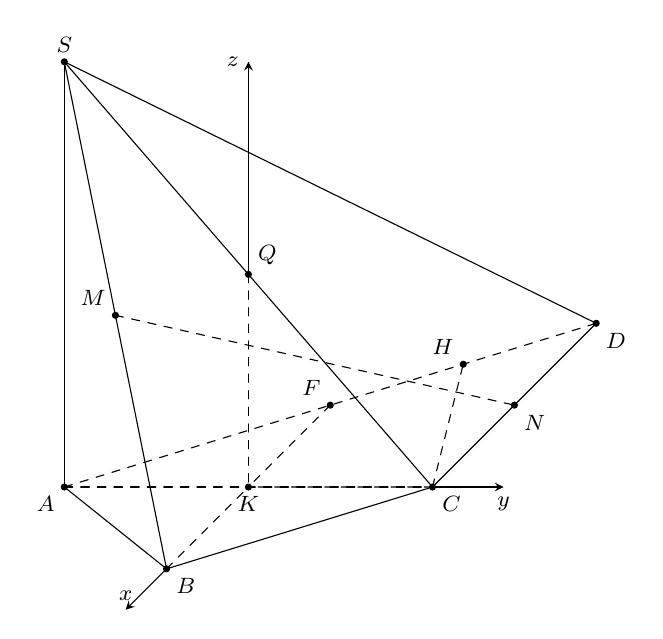
\begin{tikzpicture}[scale=2.7,font=\footnotesize,line join=round,line cap=round,>=stealth]
					\coordinate (K)  at (0,0,0);
					 \coordinate (B) at (0,0,1);
					 \coordinate (C) at (0.866,0,0);
					\coordinate  (D) at (0.866,0,-2);
					\coordinate (A) at  (-0.866,0,0);
					 \coordinate (S) at (-0.866,2,0);
					 \coordinate (M) at (-0.433,1,0.5);
					 \coordinate (N) at (0.866,0,-1);
					\coordinate (H) at (0.433,0,-1.5); 
					 \coordinate (Q) at (0,1,0);
					\coordinate (F) at (0,0,-1); 
					\draw (A) --  (B) -- (C) -- (D);
					\draw[dashed]  (A) -- (C);
					\draw  (S) -- (A);
					\draw (S) -- (B); 
					\draw (S)  -- (C);
					 \draw (S) -- (D);
					 \draw[dashed] (M) -- (N);
					\draw[dashed] (B) -- (K); 
					\draw[dashed] (A)  -- (K);
					\draw[dashed] (C) --  (K)
						(A) -- (D); 
					 \draw[dashed] (C) -- (H);
					\draw[dashed] (F)  -- (K);
					\draw[dashed]  (Q) -- (K);
					\foreach \pt  in {A,B,C,D,S,K,M,N,Q,F,H}
					\filldraw (\pt)  circle (0.4pt);
					\node[below left] at  (A) {$A$};
					\node[below right] at (B) {$B$}; 
					\node[below right] at (C)  {$C$};
					\node[below right] at  (D) {$D$};
					\node[above] at  (S) {$S$};
					\node[below] at (K) {$K$}; 
					\node[above left] at (M)  {$M$};
					 \node[below right] at (N) {$N$};
					\node[above left] at  (H) {$H$};
					\node[above right]  at (Q) {$Q$};
					\node[above left]  at (F) {$F$};
					\draw[->] (0.866,0,0) -- (1.2,0,0) node[below] {$y$}; 
					\draw[->] (0,1,0) -- (0,2,0) node[left] {$z$}; 
					\draw[->] (0,0,1) -- (0,0,1.5) node[above]  {$x$};
				\end{tikzpicture}
		\end{center}
		Ta có 
		$K(0;0;0)$, $B\left(\dfrac{a}{2};0;0\right)$, $C\left(0;\dfrac{a\sqrt{3}}{2};0\right)$, $A\left(0;-\dfrac{a\sqrt{3}}{2};0\right)$, 
		 $S\left(0;-\dfrac{a\sqrt{3}}{2};a\right)$, $N\left(-\dfrac{a}{2};\dfrac{a\sqrt{3}}{2};0\right)$,\\ $M\left(\dfrac{a}{4};-\dfrac{a\sqrt{3}}{2};\dfrac{a}{2}\right)$.\\
		Véc-tơ $\vec{MN} = \left(-\dfrac{3a}{4}; \dfrac{3a\sqrt{3}}{4}; -\dfrac{a}{2}\right)$.\\ 
		Chọn $\vec{u}_1 = (-3; 3\sqrt{3};  -2)$ cùng phương với $\vec{MN}$.\\
		\textit{Nhận  xét}
		 $$\heva{&BK \perp SA\\&BK \perp AC}\Rightarrow BK \perp (SAC).$$
		Vectơ  $\vec{BK} = \left(-\dfrac{a}{2}; 0; 0\right)$ là véc-tơ pháp tuyến của mặt phẳng $(SAC)$ nên ta chọn $\vec{n}_1 = (1;0;0)$ cùng phương với $\vec{BK}$.\\
		Gọi $\alpha$ là góc giữa $MN$ và $(SAC)$, khi đó 
		 $$
		\sin\alpha = \dfrac{\left|\vec{u}_1 \cdot \vec{n}_1\right|}{\left|\vec{u}_1\right| \cdot  \left|\vec{n}_1\right|} = \dfrac{3\sqrt{10}}{20} \Rightarrow \cos\alpha = \dfrac{\sqrt{310}}{20}.
		 $$
	} 
\end{ex}

% nguồn: Ok_TuanLuan_Toan11_Lan2
\begin{ex}%[2H5V2-7]%[ma:0b71c119]
	Cho hình chóp tứ giác đều $S.ABCD$ có tất cả các cạnh bằng nhau. Gọi $E, M$ lần lượt là trung điểm các cạnh $BC$, $SA$ và $\alpha$ là góc tạo bởi đường thẳng $EM$ và mặt phẳng $(SBD)$. Tính  $\tan\alpha$.
	\loigiai{ 
		Chọn hệ trục tọa độ  $Oxyz$ sao cho
		$$ 
		Ox \equiv OC,\quad Oy  \equiv OB,\quad Oz \equiv OS. \text{ Chọn } OA=1.
		 $$
		Ta có 
		$ 
		C(1;0;0)$, $A(-1;0;0) $, $ \vec{AC} = (2;0;0) 
		\Rightarrow \text{Véc-tơ pháp tuyến của mặt phẳng }  (SBD) \text{ là } \vec{n} = (2;0;0)
		 $.\\
		Từ $SA = AB = OA\sqrt{2} = \sqrt{2} \Rightarrow SO = \sqrt{SA^2  - OA^2} = 1$\\
		Suy ra  $S(0;0;1)$, $M = \left(-\dfrac{1}{2};0;\dfrac{1}{2}\right)$.
		\begin{center}
			 \tdplotsetmaincoords{70}{110}
			\begin{tikzpicture}[tdplot_main_coords,scale=4.0]
					\pgfmathsetmacro{\a}{1} 
					\coordinate (O) at  (0,0,0);
					\coordinate (C) at  (\a,0,0);
					\coordinate (A) at  (-\a,0,0);
					\coordinate (B)  at (0,\a,0);
					\coordinate (D) at (0,-\a,0); 
					 \coordinate (S) at (0,0,\a);
					\coordinate (E)  at (0.5*\a,0.5*\a,0);
					\coordinate (M) at (-0.5*\a,0,0.5*\a); 
					\draw[dashed] (A) -- (D); 
					\draw[dashed] (A)  -- (B);
					\draw  (B) -- (C);
					\draw (C)  -- (D);
					\draw[dashed]  (S) -- (A);
					\draw  (S) -- (B);
					 \draw (S) -- (C);
					\draw (S)  -- (D);
					\draw[dashed] (O) --  (A);
					\draw[dashed]  (O) -- (D);
					\draw[dashed] (O) --  (B);
					\draw[dashed] (O) --  (C);
					\draw[dashed] (S) --  (O);
					\draw[dashed] (E)  -- (M);
					\foreach \point/\pos  in {O/below right,S/right,A/below,B/below right,C/below right,D/below left,E/above right,M/left}
					\fill (\point) circle (0.5pt) node[\pos]  {$\point$};
					\draw[->] (C)  -- (1.5*\a,0,0) node[below] {$x$};
					 \draw[->] (B) -- (0,1.5*\a,0) node[left] {$y$};
					 \draw[->] (S) -- (0,0,1.5*\a) node[above] {$z$};
				\end{tikzpicture}
		\end{center}
		Ta  có $C(1;0;0)$, $ B(0;1;0) \Rightarrow E\left(\dfrac{1}{2}; \dfrac{1}{2}; 0\right)$.\\
		$\Rightarrow \vec{EM} = \left(1; \dfrac{1}{2}; -\dfrac{1}{2}\right)$ là vectơ  chỉ phương của đường thẳng $EM$.\\
		Suy ra 
		 $$
		\sin\left(EM, (SBD)\right) = \dfrac{\left|\vec{ME} \cdot \vec{AC}\right|}{\left|\vec{ME}\right| \cdot \left|\vec{AC}\right|} =  \dfrac{2}{\sqrt{1^2 + \left(\dfrac{1}{2}\right)^2 + \left(-\dfrac{1}{2}\right)^2} \cdot 2} = \dfrac{\sqrt{6}}{3}.
		 $$
		Do đó 
		$ \cos\alpha =  \dfrac{1}{\sqrt{3}} \Rightarrow \tan\alpha = \sqrt{2}$.
	} 
\end{ex}

% nguồn: Ok_TuanLuan_Toan11_Lan2
\begin{ex}%[2H5V2-7]%[ma:17651df7]
	Cho lăng trụ tứ giác đều $ABCD.A_1B_1C_1D_1$ cạnh đáy bằng $1$ và chiều cao bằng  $x$. Tìm $x$ để góc tạo bởi đường thẳng $B_1D$ và $(B_1D_1C)$ đạt giá trị lớn nhất.
	\loigiai{ 
		Chọn hệ trục tọa độ $Oxyz$ sao cho $O \equiv D_1$, $ C_1$ thuộc trục $Ox$, $A_1$ thuộc  $Oy$, $D$ thuộc $Oz$ như hình vẽ.\\
		 Khi đó tọa độ các điểm
		$ 
		D_1(0;0;0)$, $ B_1(1;1;0)$, $  D(0;0;x)$, $ C(1;0;x)
		$. 
		\begin{center}
			 \tdplotsetmaincoords{70}{110}
			\begin{tikzpicture}[tdplot_main_coords,scale=4]
					\coordinate (D1) at (0,0,0); 
					\coordinate (C1) at  (1,0,0);
					\coordinate (A1)  at (0,1,0);
					\coordinate  (D) at (0,0,1);
					\coordinate (B1) at  (1,1,0);
					\coordinate (A)  at (0,1,1);
					\coordinate  (B) at (1,1,1);
					\coordinate (C) at (1,0,1); 
					\draw[->] (C1)  -- (1.5,0,0) node[right] {$x$};
					\draw[->] (A1) -- (0,1.5,0) node[above]  {$y$};
					\draw[->] (D) -- (0,0,1.5) node[left] {$z$}; 
					\draw (C1) -- (B1) -- (A1); 
					 \draw (C) -- (B) -- (A);
					\draw  (C) -- (C1);
					\draw (B)  -- (B1);
					\draw (A) -- (A1); 
					\draw  (D) -- (A);
					 \draw (D) -- (C);
					 \draw[dashed] (D1) -- (C1);
					\draw[dashed] (D1) --  (A1);
					 \draw[dashed] (D1) -- (D);
					\draw[dashed] (B1) --  (D);
					 \draw[dashed] (B1) -- (C);
					 \node[left] at (D1) {$D_1$};
					\node[left] at  (C1) {$C_1$};
					 \node[below right] at (A1) {$A_1$};
					\node[above left]  at (D) {$D$};
					\node[below]  at (B1) {$B_1$};
					 \node[above left] at (A) {$A$};
					\node[left] at  (C) {$C$};
					\node[left] at  (B) {$B$};
				\end{tikzpicture}
		\end{center}
		Mặt phẳng $(B_1D_1C)$ nhận vectơ  pháp tuyến
		$$ 
		\vec{n} =  \left[\vec{D_1B_1}, \vec{D_1C}\right] = \left[(1;1;0), (1;0;x)\right] = (x; -x; -1).
		 $$
		Đường thẳng $B_1D$ có vectơ  chỉ phương
		$$ 
		\vec{u} = \vec{DB_1} =  (1;1;-x).
		$$ 
		Gọi $\varphi$ là góc giữa $B_1D$ và $(B_1D_1C)$, khi  đó
		$$ 
		\sin\varphi = \dfrac{\left|\vec{u} \cdot \vec{n}\right|}{\left|\vec{u}\right| \cdot \left|\vec{n}\right|} = \dfrac{\left|x - x + x\right|}{\sqrt{1^2 + 1^2 + x^2} \cdot \sqrt{x^2 + x^2 + 1}} = \dfrac{x}{\sqrt{x^2 + 2} \cdot \sqrt{2x^2 + 1}}= \dfrac{x}{\sqrt{\left(2x^2 + 1\right)\left(x^2 + 2\right)}}  \quad (x > 0).
		$$ 
		Đặt $f(x) =  \sin\varphi$.
		$$ 
		\dfrac{1}{\sqrt{\left(2x  + \dfrac{1}{x} \right) \left(x + \dfrac{2}{x} \right)}}
		= \dfrac{1}{\sqrt{2 \left(x^2 + \dfrac{1}{x^2} \right)  + 5}}
		\leq \dfrac{1}{\sqrt{2 \cdot 2 \cdot \sqrt{x^2 \cdot \dfrac{1}{x^2} } + 5}} = \dfrac{1}{3}. 
		$$ 
		Do đó 
		$$ 
		f(x) = \dfrac{x}{\sqrt{x^2 + 2}  \cdot \sqrt{2x^2 + 1}} \le \dfrac{1}{3}.
		 $$
		Dấu $"="$ xảy ra khi  $x = 1$.\\
		Vậy góc tạo bởi $B_1D$ và $(B_1D_1C)$  đạt giá trị lớn nhất khi $x = 1$.
	 }
\end{ex}

% nguồn: Ok_TuanLuan_Toan11_Lan2
\begin{ex}%[2H5V2-7]%[ma:3a77f58a]
	Cho hình chóp $S.ABC$ có đáy $ABC$ là tam giác vuông cân tại $B$, $BC = a$. Cạnh bên $SA$ vuông góc  với đáy và $SA = a\sqrt{3}$. Gọi $M$ là trung điểm $AC$. Tính $\cot$ của góc giữa hai mặt phẳng $(SBM)$ và $(SAB)$.
	\loigiai{ 
		Chọn hệ trục tọa độ  như hình vẽ
		\begin{center}
			 \tdplotsetmaincoords{70}{110}
			\begin{tikzpicture}[tdplot_main_coords,scale=2.5]
					\coordinate  (A) at (0,0,0);
					 \coordinate (B) at (1.5,0,0);
					 \coordinate (C) at (0,1.5,0);
					\coordinate (S) at  (0,0,2);
					\coordinate (M) at  (0,0.75,0);
					\draw[dashed,->] (0,0,0) -- (-2,0,0) node[below] {$x$}; 
					\draw[->]  (0,1.5,0) -- (-0.5,2,0) node[right] {$y$};
					\draw[->] (1.5,0,0) --  (1.5,0,3) node[above] {$z$};
					\draw[dashed] (B)  -- (A) -- (C)
						(S)  -- (A);
					\draw (B) -- (C); 
					\draw (S)  -- (B);
					 \draw (S) -- (C);
					\draw[dashed] (B) -- (M); 
					\draw[dashed] (S)  -- (M);
					\fill (A) circle (0.5pt) node[below left] {$A$}; 
					 \fill (B) circle (0.5pt) node[below] {$B$};
					\fill (C) circle (0.5pt) node[below  right] {$C$};
					\fill  (S) circle (0.5pt) node[above] {$S$};
					\fill (M) circle (0.5pt) node[below left] {$M$}; 
				\end{tikzpicture}
		\end{center}
		Tọa độ các điểm 
		$ 
		B(0;0;0)$, $ A(a;0;0)$, $ C(0;a;0)$, $ S\left(a,0;a\sqrt{3}\right)$, $ M\left(\dfrac{a}{2}; \dfrac{a}{2}; 0\right)$.\\ 
		 Ta có
		\begin{align*}
			\vec{n}_{(SAB)} &=  (0;1;0).\\
			\vec{n}_{(SBM)} &= \left[\vec{SB}, \vec{MB}\right] = \left(a(1;0;\sqrt{3})\right)  \wedge \left(\dfrac{a}{2}(1;1;0)\right) = \dfrac{a^2}{2}\left(-\sqrt{3};\sqrt{3};1\right).
		\end{align*}
		Đặt góc giữa $(SBM)$ và $(SAB)$ là $\alpha$,  ta có
		$$ 
		\left|\cos\alpha\right| =  \dfrac{\left|\vec{n}_{(SAB)} \cdot \vec{n}_{(SBM)}\right|}{\left|\vec{n}_{(SAB)}\right|\cdot \left|\vec{n}_{(SBM)}\right|} = \dfrac{\sqrt{21}}{7}.
		 $$
		 Khi đó
		$$ 
		\sin\alpha = \sqrt{1 - \left(\dfrac{\sqrt{21}}{7}\right)^2} = \dfrac{2\sqrt{7}}{7} \Rightarrow \cot\alpha = \dfrac{\cos\alpha}{\sin\alpha} =  \dfrac{\sqrt{3}}{2}.
		 $$
	 }
\end{ex}

% nguồn: Phan2_Lop_12_Hinh_hoc_Chuong_5
\begin{bt}%[2H5V2-7]%[ma:de66e11a]
	Cho hình chóp $S.ABCD$ có đáy $ABCD$ là hình thang cân, $AD = 2AB = 2BC = 2CD =  2a$. Hai mặt phẳng $(SAB)$ và $(SAD)$ cùng vuông góc với mặt phẳng $(ABCD)$. Gọi $M$, $N$ lần lượt là trung điểm của $SB$ và $CD$. Tính cosin góc giữa $MN$ và $(SAC)$, biết thể tích khối chóp $S.ABCD$ bằng $\dfrac{a^3\sqrt{3}}{4}$.
	 \loigiai{
		Vì $ABCD$ là hình thang cân có $AD = 2AB = 2BC = 2CD = 2a$.\\ 
		Suy ra $AD = 2a$, $AB = BC =  CD = a \Rightarrow CH = \dfrac{a\sqrt{3}}{2}$.\\
		$S_{ABCD}  = \dfrac{a + 2a}{2} \cdot \dfrac{a\sqrt{3}}{2} = \dfrac{3\sqrt{3}a^2}{4}$.\\
		Nên $V_{ABCD} =  \dfrac{1}{3} \cdot \dfrac{3\sqrt{3}a^2}{4} \cdot SA = \dfrac{a^2\sqrt{3}}{4} \Rightarrow SA = a$.\\
		Gọi $F$ là trung điểm của $AD$, khi đó $CF=AF=AB=BC=a\Rightarrow $  Tứ giác $ABCF$ là hình thoi.\\
		Do đó $AC\perp  BF$.\\
		Gắn hình chóp vào hệ trục  tọa độ như hình vẽ dưới đây
		\begin{center}
			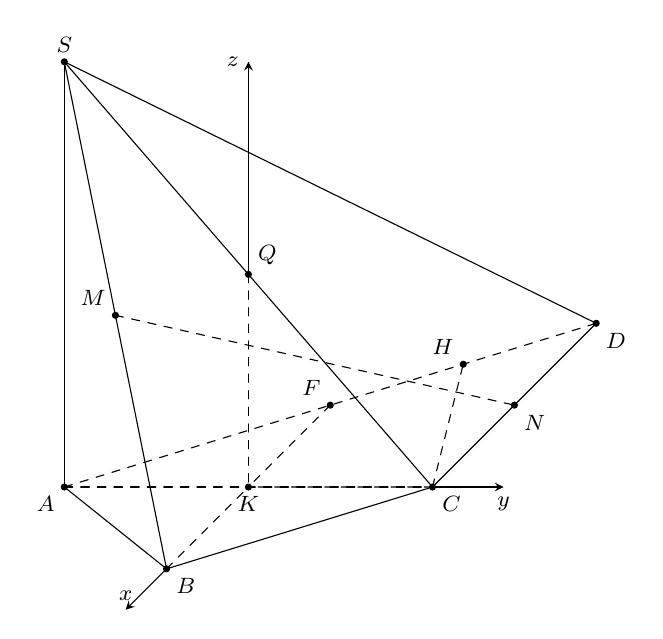
\begin{tikzpicture}[scale=2.7,font=\footnotesize,line join=round,line cap=round,>=stealth]
					\coordinate (K)  at (0,0,0);
					\coordinate  (B) at (0,0,1);
					\coordinate  (C) at (0.866,0,0);
					\coordinate (D) at (0.866,0,-2); 
					 \coordinate (A) at (-0.866,0,0);
					\coordinate (S)  at (-0.866,2,0);
					\coordinate (M)  at (-0.433,1,0.5);
					 \coordinate (N) at (0.866,0,-1);
					\coordinate  (H) at (0.433,0,-1.5);
					\coordinate (Q) at (0,1,0); 
					\coordinate (F) at  (0,0,-1);
					\draw (A) -- (B) --  (C) -- (D);
					\draw[dashed] (A) --  (C);
					\draw  (S) -- (A);
					\draw  (S) -- (B);
					\draw (S) -- (C); 
					 \draw (S) -- (D);
					\draw[dashed] (M) -- (N); 
					\draw[dashed] (B) -- (K); 
					\draw[dashed] (A)  -- (K);
					\draw[dashed] (C) -- (K) 
						(A)  -- (D);
					\draw[dashed] (C) --  (H);
					\draw[dashed] (F)  -- (K);
					\draw[dashed] (Q)  -- (K);
					\foreach \pt in {A,B,C,D,S,K,M,N,Q,F,H} 
					\filldraw (\pt) circle  (0.4pt);
					\node[below left] at  (A) {$A$};
					\node[below right] at (B)  {$B$};
					\node[below  right] at (C) {$C$};
					 \node[below right] at (D) {$D$};
					\node[above]  at (S) {$S$};
					\node[below] at (K) {$K$}; 
					\node[above left] at  (M) {$M$};
					\node[below right] at  (N) {$N$};
					\node[above left] at (H)  {$H$};
					\node[above  right] at (Q) {$Q$};
					\node[above left] at (F) {$F$}; 
					\draw[->] (0.866,0,0)  -- (1.2,0,0) node[below] {$y$};
					\draw[->] (0,1,0) --  (0,2,0) node[left] {$z$};
					\draw[->]  (0,0,1) -- (0,0,1.5) node[above] {$x$};
				\end{tikzpicture}
		\end{center}
		Ta có 
		$K(0;0;0)$, $B\left(\dfrac{a}{2};0;0\right)$,  $C\left(0;\dfrac{a\sqrt{3}}{2};0\right)$, $A\left(0;-\dfrac{a\sqrt{3}}{2};0\right)$,
		 $S\left(0;-\dfrac{a\sqrt{3}}{2};a\right)$, $N\left(-\dfrac{a}{2};\dfrac{a\sqrt{3}}{2};0\right)$,\\ $M\left(\dfrac{a}{4};-\dfrac{a\sqrt{3}}{2};\dfrac{a}{2}\right)$.\\
		Véc-tơ $\vec{MN} = \left(-\dfrac{3a}{4}; \dfrac{3a\sqrt{3}}{4}; -\dfrac{a}{2}\right)$.\\ 
		Chọn $\vec{u}_1 = (-3; 3\sqrt{3}; -2)$ cùng  phương với $\vec{MN}$.\\
		 \textit{Nhận xét}
		$$\heva{&BK \perp SA\\&BK \perp AC}\Rightarrow BK \perp  (SAC).$$
		Vectơ $\vec{BK} = \left(-\dfrac{a}{2}; 0; 0\right)$ là véc-tơ pháp tuyến của mặt phẳng  $(SAC)$ nên ta chọn $\vec{n}_1 = (1;0;0)$ cùng phương với $\vec{BK}$.\\
		Gọi $\alpha$ là góc giữa $MN$ và $(SAC)$, khi  đó
		$$ 
		\sin\alpha = \dfrac{\left|\vec{u}_1 \cdot \vec{n}_1\right|}{\left|\vec{u}_1\right| \cdot \left|\vec{n}_1\right|} = \dfrac{3\sqrt{10}}{20} \Rightarrow \cos\alpha =  \dfrac{\sqrt{310}}{20}.
		 $$
	} 
\end{bt}

% nguồn: Phan2_Lop_12_Hinh_hoc_Chuong_5
\begin{bt}%[2H5V2-7]%[ma:ada34a82]
	Cho lăng trụ tứ giác đều $ABCD.A_1B_1C_1D_1$ cạnh đáy bằng $1$ và chiều cao bằng $x$.  Tìm $x$ để góc tạo bởi đường thẳng $B_1D$ và $(B_1D_1C)$ đạt giá trị lớn nhất.
	 \loigiai{
		Chọn hệ trục tọa độ $Oxyz$ sao  cho $O \equiv D_1$, $ C_1$ thuộc trục $Ox$, $A_1$ thuộc $Oy$, $D$ thuộc $Oz$ như hình vẽ.\\
		Khi đó  tọa độ các điểm
		$ 
		D_1(0;0;0)$, $ B_1(1;1;0)$,  $ D(0;0;x)$, $ C(1;0;x)
		$. 
		\begin{center}
			 \tdplotsetmaincoords{70}{110}
			\begin{tikzpicture}[tdplot_main_coords,scale=4]
					\coordinate (D1)  at (0,0,0);
					\coordinate  (C1) at (1,0,0);
					\coordinate (A1) at (0,1,0); 
					\coordinate (D) at  (0,0,1);
					\coordinate  (B1) at (1,1,0);
					\coordinate (A) at  (0,1,1);
					 \coordinate (B) at (1,1,1);
					\coordinate (C) at (1,0,1); 
					\draw[->] (C1) --  (1.5,0,0) node[right] {$x$};
					\draw[->] (A1) -- (0,1.5,0) node[above]  {$y$};
					\draw[->]  (D) -- (0,0,1.5) node[left] {$z$};
					\draw (C1) -- (B1)  -- (A1);
					 \draw (C) -- (B) -- (A);
					 \draw (C) -- (C1);
					\draw (B)  -- (B1);
					\draw (A) --  (A1);
					\draw (D)  -- (A);
					 \draw (D) -- (C);
					\draw[dashed] (D1)  -- (C1);
					 \draw[dashed] (D1) -- (A1);
					\draw[dashed] (D1)  -- (D);
					\draw[dashed]  (B1) -- (D);
					\draw[dashed] (B1) --  (C);
					\node[left] at (D1) {$D_1$}; 
					\node[left] at (C1) {$C_1$}; 
					\node[below right] at (A1) {$A_1$}; 
					 \node[above left] at (D) {$D$};
					\node[below] at  (B1) {$B_1$};
					\node[above left]  at (A) {$A$};
					\node[left] at  (C) {$C$};
					\node[left] at (B)  {$B$};
				\end{tikzpicture}
		\end{center}
		 Mặt phẳng $(B_1D_1C)$ nhận vectơ pháp tuyến
		$$ 
		\vec{n} = \left[\vec{D_1B_1},  \vec{D_1C}\right] = \left[(1;1;0), (1;0;x)\right] = (x; -x; -1).
		$$ 
		Đường thẳng $B_1D$ có vectơ chỉ  phương
		 $$
		\vec{u}  = \vec{DB_1} = (1;1;-x).
		$$ 
		Gọi $\varphi$ là góc giữa $B_1D$ và  $(B_1D_1C)$, khi đó
		$$ 
		\sin\varphi = \dfrac{\left|\vec{u} \cdot \vec{n}\right|}{\left|\vec{u}\right| \cdot \left|\vec{n}\right|} = \dfrac{\left|x - x + x\right|}{\sqrt{1^2 + 1^2 +  x^2} \cdot \sqrt{x^2 + x^2 + 1}} = \dfrac{x}{\sqrt{x^2 + 2} \cdot \sqrt{2x^2 + 1}}= \dfrac{x}{\sqrt{\left(2x^2 + 1\right)\left(x^2 + 2\right)}} \quad (x > 0).
		$$ 
		 Đặt $f(x) = \sin\varphi$.
		 $$
		\dfrac{1}{\sqrt{\left(2x  + \dfrac{1}{x} \right) \left(x + \dfrac{2}{x} \right)}}
		= \dfrac{1}{\sqrt{2 \left(x^2  + \dfrac{1}{x^2} \right) + 5}}
		\leq \dfrac{1}{\sqrt{2 \cdot 2  \cdot \sqrt{x^2 \cdot \dfrac{1}{x^2} } + 5}} = \dfrac{1}{3}.
		$$ 
		Do đó 
		 $$
		f(x) = \dfrac{x}{\sqrt{x^2 + 2} \cdot \sqrt{2x^2 +  1}} \le \dfrac{1}{3}.
		 $$
		Dấu $"="$ xảy  ra khi $x = 1$.\\
		Vậy góc tạo bởi $B_1D$ và $(B_1D_1C)$ đạt giá trị lớn  nhất khi $x = 1$.
	} 
\end{bt}

% nguồn: Phan2_Lop_12_Hinh_hoc_Chuong_5
\begin{bt}%[2H5V2-7]%[ma:27c9a7d7]
	Trong một khung lưới ô vuông gồm các hình lập phương,  xét các đường thẳng đi qua hai nút lưới (mỗi nút lưới là đỉnh của hình lập phương), người ta đưa ra một cách kiểm tra độ lệch về phương của hai đường thẳng bằng cách gắn hệ tọa độ $Oxyz$ vào khung lưới ô vuông và tìm vectơ chỉ phương của hai đường thẳng đó. Giả sử, đường thẳng $a$ đi qua hai nút lưới $M(1; 1; 2)$ và $N(0; 3; 0)$, đường thẳng $b$ đi qua hai nút lưới $P(1; 0; 3)$ và $Q(3; 3; 9)$. Sau khi làm tròn đến hàng đơn vị của độ thì góc giữa hai đường thẳng $a$ và $b$ bằng $n^\circ$ ($n$ là số tự nhiên). Giá trị của $n$ bằng bao nhiêu?
	 \loigiai{
		Ta  có $\overrightarrow{MN}=(-1; 2;-2), \overrightarrow{PQ}=(2; 3; 6)$.
		Khi đó: $\cos(a, b)=\dfrac{|\overrightarrow{MN} \cdot \overrightarrow{PQ}|}{|\overrightarrow{MN}|\cdot|\overrightarrow{PQ}|}=\dfrac{8}{21}$, suy ra $(a, b) \approx 68^\circ$. 
	 }
\end{bt}

% nguồn: Phan2_Lop_12_Hinh_hoc_Chuong_5
\begin{bt}%[2H5V2-7]%[ma:8ccf6f74]
	Cho hình chóp $S.ABC$ có đáy $ABC$ là tam giác vuông cân tại $B$, $BC = a$. Cạnh bên $SA$ vuông góc với đáy  và $SA = a\sqrt{3}$. Gọi $M$ là trung điểm $AC$. Tính $\cot$ của góc giữa hai mặt phẳng $(SBM)$ và $(SAB)$.
	 \loigiai{
		Chọn hệ trục tọa độ  như hình vẽ
		\begin{center}
			\tdplotsetmaincoords{70}{110} 
			\begin{tikzpicture}[tdplot_main_coords,scale=2.5]
					\coordinate (A) at (0,0,0); 
					\coordinate (B) at (1.5,0,0); 
					 \coordinate (C) at (0,1.5,0);
					\coordinate (S)  at (0,0,2);
					\coordinate (M) at  (0,0.75,0);
					\draw[dashed,->] (0,0,0) --  (-2,0,0) node[below] {$x$};
					\draw[->] (0,1.5,0) -- (-0.5,2,0)  node[right] {$y$};
					\draw[->] (1.5,0,0)  -- (1.5,0,3) node[above] {$z$};
					\draw[dashed] (B) --  (A) -- (C)
						(S) -- (A); 
					\draw (B) --  (C);
					\draw (S) --  (B);
					 \draw (S) -- (C);
					\draw[dashed] (B) -- (M); 
					\draw[dashed] (S)  -- (M);
					\fill (A) circle (0.5pt) node[below left] {$A$}; 
					\fill  (B) circle (0.5pt) node[below] {$B$};
					\fill (C)  circle (0.5pt) node[below right] {$C$};
					\fill (S) circle (0.5pt) node[above]  {$S$};
					\fill (M)  circle (0.5pt) node[below left] {$M$};
				\end{tikzpicture}
		\end{center}
		 Tọa độ các điểm
		$ 
		B(0;0;0)$, $ A(a;0;0)$, $ C(0;a;0)$, $ S\left(a,0;a\sqrt{3}\right)$,  $ M\left(\dfrac{a}{2}; \dfrac{a}{2}; 0\right)$.\\
		 Ta có
		\begin{align*}
			\vec{n}_{(SAB)}  &= (0;1;0).\\
			\vec{n}_{(SBM)} &= \left[\vec{SB}, \vec{MB}\right] = \left(a(1;0;\sqrt{3})\right) \wedge \left(\dfrac{a}{2}(1;1;0)\right) = \dfrac{a^2}{2}\left(-\sqrt{3};\sqrt{3};1\right). 
		\end{align*}
		Đặt góc giữa  $(SBM)$ và $(SAB)$ là $\alpha$, ta có
		 $$
		\left|\cos\alpha\right| = \dfrac{\left|\vec{n}_{(SAB)}  \cdot \vec{n}_{(SBM)}\right|}{\left|\vec{n}_{(SAB)}\right|\cdot \left|\vec{n}_{(SBM)}\right|} = \dfrac{\sqrt{21}}{7}.
		$$ 
		Khi  đó
		 $$
		\sin\alpha = \sqrt{1 - \left(\dfrac{\sqrt{21}}{7}\right)^2}  = \dfrac{2\sqrt{7}}{7} \Rightarrow \cot\alpha = \dfrac{\cos\alpha}{\sin\alpha} = \dfrac{\sqrt{3}}{2}.
		$$ 
	} 
\end{bt}

% nguồn: Phan2_Lop_12_Hinh_hoc_Chuong_5
\begin{bt}%[2H5V2-7]%[ma:f93be5b2]
	Cho hình chóp tứ giác đều $S.ABCD$ có tất cả các  cạnh bằng nhau. Gọi $E, M$ lần lượt là trung điểm các cạnh $BC$, $SA$ và $\alpha$ là góc tạo bởi đường thẳng $EM$ và mặt phẳng $(SBD)$. Tính $\tan\alpha$.
	\loigiai{ 
		Chọn hệ trục tọa độ $Oxyz$ sao  cho
		$$ 
		Ox \equiv OC,\quad  Oy \equiv OB,\quad Oz \equiv OS. \text{ Chọn } OA=1.
		 $$
		Ta có 
		$ 
		C(1;0;0)$, $A(-1;0;0) $, $ \vec{AC}  = (2;0;0)
		\Rightarrow \text{ Véc-tơ pháp tuyến của mặt phẳng } (SBD)  \text{ là } \vec{n} = (2;0;0)
		$.\\ 
		Từ  $SA = AB = OA\sqrt{2} = \sqrt{2} \Rightarrow SO = \sqrt{SA^2 - OA^2} = 1$\\
		 Suy ra $S(0;0;1)$, $M = \left(-\dfrac{1}{2};0;\dfrac{1}{2}\right)$.
		\begin{center}
			 \tdplotsetmaincoords{70}{110}
			\begin{tikzpicture}[tdplot_main_coords,scale=4.0]
					\pgfmathsetmacro{\a}{1} 
					\coordinate (O)  at (0,0,0);
					 \coordinate (C) at (\a,0,0);
					\coordinate  (A) at (-\a,0,0);
					\coordinate (B)  at (0,\a,0);
					 \coordinate (D) at (0,-\a,0);
					\coordinate (S)  at (0,0,\a);
					\coordinate (E)  at (0.5*\a,0.5*\a,0);
					\coordinate (M) at (-0.5*\a,0,0.5*\a); 
					\draw[dashed] (A) -- (D); 
					\draw[dashed] (A) --  (B);
					\draw (B)  -- (C);
					\draw (C) --  (D);
					 \draw[dashed] (S) -- (A);
					\draw (S) --  (B);
					 \draw (S) -- (C);
					\draw (S) -- (D); 
					\draw[dashed]  (O) -- (A);
					\draw[dashed] (O) -- (D); 
					\draw[dashed] (O) --  (B);
					\draw[dashed] (O) --  (C);
					\draw[dashed] (S) --  (O);
					\draw[dashed]  (E) -- (M);
					\foreach \point/\pos in {O/below right,S/right,A/below,B/below right,C/below right,D/below  left,E/above right,M/left}
					 \fill (\point) circle (0.5pt) node[\pos] {$\point$};
					\draw[->] (C) -- (1.5*\a,0,0) node[below]  {$x$};
					\draw[->] (B) --  (0,1.5*\a,0) node[left] {$y$};
					 \draw[->] (S) -- (0,0,1.5*\a) node[above] {$z$};
				\end{tikzpicture}
		\end{center}
		 Ta có $C(1;0;0)$, $ B(0;1;0) \Rightarrow E\left(\dfrac{1}{2}; \dfrac{1}{2}; 0\right)$.\\
		$\Rightarrow \vec{EM} = \left(1; \dfrac{1}{2}; -\dfrac{1}{2}\right)$ là vectơ chỉ phương của đường thẳng  $EM$.\\
		Suy ra 
		 $$
		\sin\left(EM, (SBD)\right) = \dfrac{\left|\vec{ME} \cdot \vec{AC}\right|}{\left|\vec{ME}\right| \cdot \left|\vec{AC}\right|} = \dfrac{2}{\sqrt{1^2 + \left(\dfrac{1}{2}\right)^2 +  \left(-\dfrac{1}{2}\right)^2} \cdot 2} = \dfrac{\sqrt{6}}{3}.
		 $$
		Do đó 
		 $ \cos\alpha = \dfrac{1}{\sqrt{3}} \Rightarrow \tan\alpha = \sqrt{2}$.
	} 
\end{bt}

% nguồn: Phan2_Lop_12_Hinh_hoc_Chuong_5
\begin{bt}%[2H5C2-7]%[ma:8967c0ae]
	Trong không gian $Oxyz$, với mặt phẳng $(Oxy)$ là mặt đất, một máy bay cất cánh từ vị trí $A(0; 10; 0)$ với vận tốc $\overrightarrow{v}=(150; 150; 40)$. Tính góc nâng của máy bay (góc giữa hướng chuyển động bay lên của máy bay với đường băng và làm tròn kết quả  đến hàng đơn vị).
	 \loigiai{
		Gọi $\Delta$ là đường thẳng biểu thị cho hướng chuyển động bay lên của máy bay.\\ 
		Ta có $\Delta$ nhận vectơ $\overrightarrow{v}=(150;  150; 40)=10(15; 15; 4)$ làm vectơ chỉ phương.\\
		Mặt phẳng $(Oxy)$ có  vectơ pháp tuyến $\overrightarrow{n}=(0; 0; 1)$.\\
		Gọi $\varphi$ là góc giữa  đường thẳng $\Delta$ và mặt phẳng $(Oxy)$.\\
		 Suy ra $\sin \varphi=|\cos(\overrightarrow{v}, \overrightarrow{n})|=\dfrac{|\overrightarrow{v} \cdot \overrightarrow{n}|}{|\overrightarrow{v}|\cdot|\overrightarrow{n}|}=\dfrac{|15\cdot 0+15\cdot 0+4\cdot 1|}{\sqrt{15^2+15^2+4^2} \cdot \sqrt{0^2+0^2+1^2}}=\dfrac{4}{\sqrt{466}}$.\\
		Vậy góc nâng của máy  bay là $\varphi \approx 11^\circ$.
	} 
\end{bt}
